% % \part{优化模型}
% % \chapter{智能优化}

% \documentclass[UTF8]{ctexbook}

% \ctexset{
%     part/number = \chinese{part}
% }
% \usepackage{multirow}
% \usepackage{amsmath}% ams 数学公式
% \usepackage{amsfonts}% ams 数学字体
% \usepackage{bbm}%重影字体
% \usepackage{amssymb,latexsym}% ams 数学符号与LaTeX数学符号
% \usepackage{mathrsfs}% 花式符号
% \usepackage{ntheorem}%定理、定义、证明
%     \theoremstyle{nonumberplain}
%     \theoremheaderfont{\bfseries}
%     \theorembodyfont{\normalfont}
%     \theoremsymbol{$\square$}
%     \newtheorem{Proof}{\hskip 2em 证明}
%     \newtheorem{theorem}{\hspace{2em}定理}[chapter]
%     \newtheorem{definition}{\hspace{2em}定义}[chapter] % 如果没有章, 只有节, 把上面的[chapter]改成[section]
%     \newtheorem{axiom}[definition]{\hspace{2em}公理}
%     \newtheorem{lemma}[definition]{\hspace{2em}引理}
%     \newtheorem{proposition}[definition]{\hspace{2em}命题}
%     \newtheorem{corollary}[definition]{\hspace{2em}推论}
%     \newtheorem{remark}{\hspace{2em}注}[chapter] %类似地定义其他“题头”. 这里“注”的编号与定义、定理等是分开的
%     \newtheorem{Assumption}{\hspace{2em}假设}[chapter]

% %算法伪代码
% %http://blog.csdn.net/lwb102063/article/details/53046265
% \usepackage{algorithm}
% \usepackage{algorithmicx}
% \usepackage{algpseudocode}
%     \floatname{algorithm}{算法}
%     \renewcommand{\algorithmicrequire}{\textbf{输入:}}
%     \renewcommand{\algorithmicensure}{\textbf{输出:}}
% % 罗马数字:示例:\rom{2}
% \makeatletter
% \newcommand*{\rom}[1]{\expandafter\@slowromancap\romannumeral #1@}
% \makeatother

% \usepackage{enumerate}%itemiz环境。\begin{enumerate}[step 1][a)]可以使用 A,a,I,i,1 作为可选项产生 \Alph,\alph,\Roman,\roman,\arabic 的效果
% \usepackage{cite}%参考文献
%     \bibliographystyle{plain}
% \usepackage{extarrows}% 带参数的箭头
% \usepackage{hyperref}% 超链接
% \usepackage{pifont}%然后在正文输入\ding{172}~\ding{211}得到相应数字,要是要①就输入:\ding{172}②就输:\ding{173}
% %\usepackage[CJKbookmarks, colorlinks, bookmarksnumbered=true,pdfstartview=FitH,linkcolor=black,citecolor=black]{hyperref}%超链接的格式设置
% \hypersetup{
%     colorlinks=false,% 去掉超链接颜色
%     pdfborder=0 0 0% 取消超链接的边框
% }
% \usepackage{graphicx}% 图片管理
% \usepackage{caption}
% \usepackage{subcaption}%并排的图各有标题
% \graphicspath{{images/}}% 设置图片搜索路径
% \usepackage{float,varwidth}% 浮动体
% \usepackage{booktabs}% 三线表
% \usepackage{fancyhdr}% 页眉设置
% \usepackage{xcolor}% 颜色宏包
% \usepackage{colortbl}% 彩色表格
% \usepackage{listings}% 代码高亮
% \usepackage{caption}% 对标题进行控制,如让\caption标题的字体缩小一号,同时数字标签使用粗体可以用:\usepackage[font=small,labelfont=bf]{caption}
% \usepackage{xfrac,upgreek}%分别是行间公式如a/b的形式(将原来的命令\frac改成\sfrac)和希腊字体的宏包的
% \usepackage{mathtools}%lgathered和rgathered环境把公式向左向右对齐
% \usepackage{tabularx}%提供自动延伸的表列,(X列格式说明符),文字过长时可以自动转行
% \usepackage{longtable}%长表格
% \usepackage{enumitem}%enumerate宏包的升级
% \usepackage{harpoon}%数学公式的矢量
% \usepackage{bookmark}%目录的书签
% \renewcommand{\headwidth}{\textwidth}%图片并排,这个要列在所有宏包的后面
% \definecolor{codegreen}{rgb}{0,0.6,0}
% \definecolor{codegray}{rgb}{0.5,0.5,0.5}
% \definecolor{codepurple}{rgb}{0.58,0,0.82}
% \definecolor{backcolour}{rgb}{0.95,0.95,0.92}
% \lstset{
%     commentstyle=\color{codegreen},
%     keywordstyle=\color{magenta},
%     numberstyle=\tiny\color{codegray},
%     stringstyle=\color{codepurple},
%     basicstyle=\footnotesize,
%     breakatwhitespace=false,% 断行只在空格处
%     breaklines=true,% 自动断行
%     captionpos=b,% 标题位置
%     keepspaces=true,
%     numbers=left,
%     numbersep=5pt,
%     showspaces=false,
%     showstringspaces=false,
%     showtabs=false,% 显示
%     tabsize=2% TAB 被当作两个空格
% }
% \topmargin=0pt\oddsidemargin=0pt\evensidemargin=0pt
% \textwidth=16.5cm\textheight=23cm\raggedbottom%我这么设置是为了缩小页边距,满足有的文字无法转行
% \pagestyle{headings}%页眉为章节标题,无页脚
% \setlength{\abovecaptionskip}{10pt}
% \setlength{\belowcaptionskip}{-15pt}%图片表格的前后距离设置
% \CTEXsetup[format={\zihao{-3}\raggedright\bfseries}]{section}%设置节的格式

% \begin{document}
% \part{优化模型}
\chapter{智能优化}

\section{问题的引入与分析}
    考虑如下2个最优化问题:1.只有边界约束(\ref{GA:引例1});2.有边界约束和不等式约束(\ref{GA:引例2})。引例1:
    \begin{align}
    \label{GA:引例1}
    \mathop{\min}\limits_{x,y}\quad &f(x,y)=x \cos(2\pi y)+y \sin(2\pi x)\\
    s.t.\quad &  -0.5\leqslant x\leqslant 3.5 \notag\\
    & -2\leqslant y\leqslant 3 \notag
    \end{align}
    \par
    用MATLAB求解上述引例1(\ref{GA:引例1})的程序如下
    \begin{lstlisting}[language = Matlab]
    %% 智能优化引例1:无约束
    %           max f(x,y)=y*sin(2*pi*x)+x*cos(2*pi*y)
    %                s.t.-0.5<=x<=3.5;  -2<=y<=3;
    %目标函数
    fun = @(x) x(1)*cos(2*pi*x(2)) + x(2)*sin(2*pi*x(1));
    [X, Y] = meshgrid(-4:0.035:4,-4:0.035:4);
    Z = arrayfun(@(x,y) fun([x y]), X, Y);
    domain = [-3 5.5 -4 5];
    % figure
    % surf(X, Y, Z, 'EdgeColor', 'none')
    % xlabel x, ylabel y, zlabel z
    figure;
    h(1) = ezcontour(@(X,Y) arrayfun(@(x,y) fun([x y]),X,Y),domain,150);
    hold on
    % Plot bounds
    lb = [-0.5 -2];
    ub = [3.5 3];
    h(2) = line([lb(1) lb(1)],[lb(2) ub(2)],'LineStyle','--');
    h(3) = line([ub(1) ub(1)],[lb(2) ub(2)],'LineStyle','--');
    h(4) = line([lb(1) ub(1)],[lb(2) lb(2)],'LineStyle','--');
    h(5) = line([lb(1) ub(1)],[ub(2) ub(2)],'LineStyle','--');
    title('目标函数及约束条件')
    x0 = [3 -1];
    opts = optimoptions('fmincon','Algorithm','sqp');
    problem = createOptimProblem('fmincon','objective', ...
        @(x) -fun(x),'x0',x0,'lb',lb,'ub',ub, ...
        'nonlcon',[],'options',opts);
    tic
    [xlocal,fvallocal] = fmincon(problem)
    toc
    %找最大值
    ind1 = find(X(1,:)<=ub(1) & X(1,:)>=lb(1));
    ind2 = find(Y(:,1)<=ub(2) & Y(:,2)>=lb(2));
    [a, row] = max(Z(ind2', ind1));%a为各列的最大值
    [fvalglobal, col] = max(a);%col为最大列
    row = row(col);%最大行
    maxIdx1 = col + ind1(1) - 1;
    maxIdx2 = row + ind2(1) - 1;
    % if Z(maxIdx2,maxIdx1) == fmax, disp('right')
    %最大值
    fvalglobal
    xglobal = [X(1,maxIdx1),Y(maxIdx2,1)]%最大值点
    h(6) = plot(xlocal(1),xlocal(2),'r*','MarkerSize',16);
    text(xlocal(1),xlocal(2),'局部极大值')
    h(7) = plot(xglobal(1),xglobal(2),'mp','MarkerSize',16);
    text(xglobal(1),xglobal(2),'全局极大值')
    %使用全局搜索方法求解
    % 1、Construct a GlobalSearch object
    gs = GlobalSearch;
    % 2、Run GlobalSearch
    tic;
    [xgs,~,~,~,solsgs] = run(gs,problem);
    toc
    xgs
    % 3、Plot GlobalSearch results using the '*' marker
    xGS = cell2mat({solsgs(:).X}');
    h(8) = scatter(xGS(:,1),xGS(:,2),'s','MarkerEdgeColor',[0 0 1],'LineWidth',1.25);
    %使用多初始点方法求解
    % 1、Construct a MultiStart object based on our GlobalSearch attributes
    ms = MultiStart;
    rng(4,'twister') % for reproducibility
    % 2、 Run the solver with 15 randomly generated points
    tic;
    [xms,~,~,~,solsms] = run(ms,problem,15);
    toc
    xms
    % 3、 Plot MultiStart results using a circle marker
    xMS = cell2mat({solsms(:).X}');
    h(9) = scatter(xMS(:,1),xMS(:,2),'o','MarkerEdgeColor',[0 0 0],'LineWidth',1.25);
    legend([h(1),h(2),h(6),h(7),h(8),h(9)],'Intensity','Bound','Local',...
       'Global','GlobalSearch','MultiStart','location','best')
    title('GlobalSearch and MultiStart Results')
    \end{lstlisting}
    \par
    上述引例1(\ref{GA:引例1})只考虑了边界约束,这是容易处理的。下面,我们在上面的模型中,添加不等式约束:引例2
    \begin{align}
    \label{GA:引例2}
    \mathop{\min}\limits_{x,y}\quad &f(x,y)=x \cos(2\pi y)+y \sin(2\pi x)\\
    s.t.\quad & (x-x_{c1})^2+(y-y_{c1})^2\leqslant r_1^2 \notag \\
    & (x-x_{c2})^2+(y-y_{c2})^2\leqslant r_2^2\notag \\
    & (x-x_{c3})^2+(y-y_{c3})^2\leqslant r_3^2\notag \\
    &  -0.5\leqslant x\leqslant 3.5\notag \\
    & -2\leqslant y\leqslant 3\notag
    \end{align}
    \par
    用Matlab求解引例2(\ref{GA:引例2})的程序如下
    \begin{lstlisting}[language=Matlab]
    %% 智能优化引例2:有约束
    %           max f(x,y)=y*sin(2*pi*x)+x*cos(2*pi*y)
    %           s.t.         -0.5<=x<=3.5;  -2<=y<=3;
    %           (x-xcoords(1)).^2 + (y-ycoords(1)).^2 <= 9;
    %           (x-xcoords(2)).^2 + (y-ycoords(2)).^2 <= 9;
    %           (x-xcoords(3)).^2 + (y-ycoords(3)).^2 <= 9;
    %目标函数
    fun = @(x) x(1)*cos(2*pi*x(2)) + x(2)*sin(2*pi*x(1));
    [X, Y] = meshgrid(-4:0.035:4,-4:0.035:4);
    Z = arrayfun(@(x,y) fun([x y]), X, Y);
    %约束条件
    xcoords = [2.4112 0.2064 1.6787];
    ycoords = [0.3957 0.3927 0.9877];
    domain = [-3 5.5 -4 5];
    figure;
    f(1) = ezcontour(@(X,Y) arrayfun(@(x,y) fun([x y]),X,Y),domain,150);
    hold on
    % Plot constraints
    g1 = @(x,y)  (x-xcoords(1)).^2 + (y-ycoords(1)).^2 - 9;
    g2 = @(x,y)  (x-xcoords(2)).^2 + (y-ycoords(2)).^2 - 9;
    g3 = @(x,y)  (x-xcoords(3)).^2 + (y-ycoords(3)).^2 - 9;
    f(2) = ezplot(g1,domain);
    f(2).Color = [0.8 0.7 0.1]; % yellow
    f(2).LineWidth = 1.5;
    f(3) = ezplot(g2,domain);
    f(3).Color = [0.3 0.7 0.5]; % green
    f(3).LineWidth = 1.5;
    f(4) = ezplot(g3,domain);
    f(4).Color = [0.4 0.4 0.6]; % blue
    f(4).LineWidth = 1.5;
    % Plot bounds
    lb = [-0.5 -2];
    ub = [3.5 3];
    f(5)=line([lb(1) lb(1)],[lb(2) ub(2)],'LineStyle','--');
    f(6)=line([ub(1) ub(1)],[lb(2) ub(2)],'LineStyle','--');
    f(7)=line([lb(1) ub(1)],[lb(2) lb(2)],'LineStyle','--');
    f(8)=line([lb(1) ub(1)],[ub(2) ub(2)],'LineStyle','--');
    title('目标函数及约束条件')
    % function [c,ceq] = apertureConstraint(x,xcoords,ycoords)
    % ceq = [];
    % c = (x(1) - xcoords).^2 + (x(2) - ycoords).^2 - 9;
    % end
    %构建约束条件函数
    FunConstraint = @(x) apertureConstraint(x,xcoords,ycoords);
    x0 = [3 -1];
    opts = optimoptions('fmincon','Algorithm','sqp');
    problem = createOptimProblem('fmincon','objective', ...
        @(x) -fun(x),'x0',x0,'lb',lb,'ub',ub, ...
        'nonlcon',FunConstraint,'options',opts);
    tic
    [xlocal,fvallocal] = fmincon(problem)
    toc
    %找最大值
    ind1 = find(X(1,:)<=ub(1) & X(1,:)>=lb(1));
    ind2 = find(Y(:,1)<=ub(2) & Y(:,2)>=lb(2));
    [a, row] = max(Z(ind2', ind1));%a为各列的最大值
    [fvalglobal, col] = max(a);%col为最大列
    row = row(col);%最大行
    maxIdx1 = col + ind1(1) - 1;
    maxIdx2 = row + ind2(1) - 1;
    % if Z(maxIdx2,maxIdx1) == fmax, disp('right')
    %最大值
    fvalglobal
    xglobal = [X(1,maxIdx1),Y(maxIdx2,1)]%最大值点
    f(9) = plot(xlocal(1),xlocal(2),'r*','MarkerSize',16);
    text(xlocal(1),xlocal(2),'局部极大值')
    f(10) = plot(xglobal(1),xglobal(2),'mp','MarkerSize',16);
    text(xglobal(1),xglobal(2),'全局极大值')
    %使用全局搜索方法求解
    % 1、Construct a GlobalSearch object
    gs = GlobalSearch;
    gs = GlobalSearch(gs,'StartPointsToRun','bounds-ineqs', ...
        'MaxWaitCycle',3,'BasinRadiusFactor',0.3);
    % 2、Run GlobalSearch
    tic;
    [xgs,~,~,~,solsgs] = run(gs,problem);
    toc
    xgs
    % 3、Plot GlobalSearch results using the '*' marker
    xGS = cell2mat({solsgs(:).X}');
    f(11) = scatter(xGS(:,1),xGS(:,2),'s','MarkerEdgeColor',[0 0 1],'LineWidth',1.25);
    %使用多初始点方法求解
    % 1、Construct a MultiStart object based on our GlobalSearch attributes
    ms = MultiStart;
    rng(4,'twister') % for reproducibility
    ms = MultiStart(ms,'UseParallel',true);% Set the UseParallel property of MultiStart
    try
        demoOpenedPool = false;
        % Create a parallel pool if one does not already exist
        % (requires Parallel Computing Toolbox)
        if max(size(gcp)) == 0 % if no pool
            parpool
            demoOpenedPool = true;
        end
    catch ME
        warning(message('globaloptim:globaloptimdemos:opticalInterferenceDemo:noPCT'));
    end
    %2、 Run the solver with 15 randomly generated points
    tic;
    [xms,~,~,~,solsms] = run(ms,problem,15);
    toc
    xms

    if demoOpenedPool
        % Make sure to delete the pool if one was created in this example
        delete(gcp) % delete the pool
    end
    %3、 Plot MultiStart results using a circle marker
    xMS = cell2mat({solsms(:).X}');
    f(12) = scatter(xMS(:,1),xMS(:,2),'o','MarkerEdgeColor',[0 0 0],'LineWidth',1.25);
    legend([f(1),f(2),f(5),f(9),f(10),f(11),f(12)],...
        'Intensity','Constraints','Bound','GlobalSearch','MultiStart','Location','best')
    title('GlobalSearch and MultiStart Results')
    \end{lstlisting}
    \par
    前面几章,我们所讨论的优化算法都是基于$x_{k+1}=x_k+{\alpha}_kd_k$,并且都有明确的步长${\alpha}_k$,明确的方向$d_k$,也即${\alpha}_k,d_k$并不存在随机性。这一部分,我们要介绍的方法都是\underline{随机化方法},也称为智能优化方法。
\section{遗传算法}
    % \ding{172}GA的基本思想
    % \par
    % \ding{173}GA的算法步骤
    % \par
    % \ding{174}GA伪代码
    % \par
    % \ding{175}GA的改进
    % \par
    % \ding{176}GA工具箱\\
    \subsection{GA的基本思想}
        \par
        1975年,Michigan大学的J.Holland教授提出"遗传算法"的概念,并出版了著作《Adaptation in Netural and Artificial systems》。J.Holland提出的遗传算法属于简单遗传算法,还处于遗传算法发展初期。大约在同一时期,FoegL和Rechenberg以及Schwefel引入了另两种基于自然演化原理的算法;演化程序和演化策略。这三种算法构成了目前演化计算领域的三大分支。
        \par
        Holland不仅设计了遗传算法,更重要的是,他运用统计决策理论对GA的搜索机理进行了理论分析,建立了著名的Schema定理和隐含并行性原理,为遗传算法的发展奠定了基础。De Jong在他的博士论文中将GA算法应用到函数优化问题,并设计了一系列遗传算法的执行策略和性能评价指标。De Jong的实时(Ontime)和非实时(Offtime)指标仍是GA性能的主要评价指标,并且论文中挑选了5个试验函数,也是目前GA数值实验中使用最多的试验函数。
        \par
        GA的发展高潮开始于20世纪80年代末,这里简略介绍GA在神经网络、机器学习中的应用。神经网络的学习包含两个过程:网络连接权重和网络拓扑结构。其中,权重的优化方法最著名的是Rumelhart提出的基于梯度下降法的反向传播算法(BP)。BP算法的最大弱点是局部极小问题和无法学习网络拓扑结构。GA应用于ANN的学习可以分为三个方面:连接权重、拓扑结构以及网络学习规划。目前,GA已广泛应用与BP网络、RBF网络、ANN网络和Kohonen特征映射等等。Holland最初设计GA的目的是在自适应学习统计中设计一种有效的搜索机制,遗传算法用于机器学习系统仍是目前GA应用上十分活跃的领域。这一方面最著名的例子就是所谓的分类系统,它是遗传算法与机器学习中经典的生产系统相结合的产物,并成功应用于石油管道设计和视觉系统的控制等。
    \subsection{GA的算法步骤}
        \subsubsection{基本定义}
            \begin{definition}[个体]
            如果就最优化问题而言,个体指$x\in R^n$,也即为优化问题的解。当然,有些个体(解)在约束内,我们称这样的个体为许可个体或可行个体,否则称为不许可个体\footnote{注:1.我们允许个体在约束外;2.如何设计约束。}。例:就引例(\ref{GA:引例1})而言,个体为$x=(x_1,x_2)$,记个体长度为$n(n=2)$。
            \end{definition}
            \begin{definition}[染色体]
            我们将个体进行一定的编码,编码后的个体称为染色体。例:对$x=(x_1,x_2)$,我们可以对$x_i\in R(i=1,2)$,设计编码长度为$l$,则编码后的染色体长度为$p=l\cdot n$。
            \end{definition}
            \begin{definition}[基因]
            染色体中每一分量的特征,如各分量的值。
            \end{definition}
            \begin{definition}[种群]
            多个个体的集合,记为$X$。如果设种群大小为$N$,则$X$为$N\times n$矩阵\footnote{考虑:1.如何生成新解(新个体)?2.如何说明新个体是优的,或者如何生产优良的新个体?}。
            \end{definition}
            \begin{definition}[适应度]
            个体对环境(要求的目标函数)或者规划问题(整体)的适应度,适应度越大,说明个体越好。由于我们一般要求最小化,所以适应度往往取目标函数的倒数或负。对于新个体的产生,我们可以通过改变个体的基因来形成新个体。而且,我们又要求新个体是优的,这与达尔文的“适者生存,优胜劣汰”的思想相吻合。
            \end{definition}
            \par
            下面,我们给出生物进化论的基本过程:
                \begin{figure}[H]
                \centering
                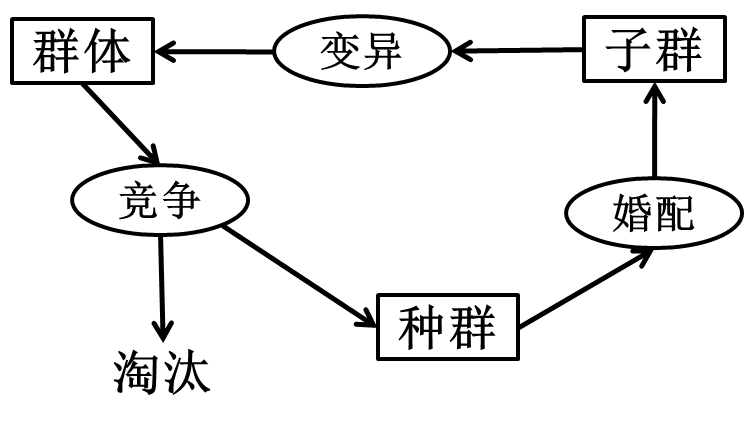
\includegraphics[width=4cm]{images/Biological_evolution.jpg}
                \caption{生物进化示意图}
                \label{fig:生物进化示意图}
                \end{figure}
            % \textcolor[rgb]{1.00,0.00,0.00}{todo:图片:生物进化示意图}
            \noindent 从上图(\ref{fig:生物进化示意图})中,可以看出,如果我们先给定一个初始种群要生产新个体(子群)而需要婚配,而子群则继承了父母双方的优良血统。那么,我们可以选择同一种群中的2个适应度高的个体进行基因交叉,以形成子群。
            \par
            例:选择适应度大的\underline{多个}个体,两两配对,进行基因交叉以生成新个体,多个新个体称为子群。子个体的产生如图(\ref{fig:子个体产生示意图})所示
        \begin{figure}[H]
        \centering
        
\includegraphics[width=5cm]{images/Sub_individual.jpg}
        \caption{子个体产生示意图}
        \label{fig:子个体产生示意图}
        \end{figure}
            % \textcolor[rgb]{1.00,0.00,0.00}{todo:图片:子个体产生示意图}
            \par
            当然,对于基因交叉,会有各种各样的方法。根据基因编码的不同,我们会有浮点数编码和二进制编码。我们可以选择以下交叉方法:
            \begin{enumerate}
            \item 适用于浮点数的交叉方法:离散重组、中间重组、线性重组等。
            \item 适用于二进制编码的交叉方法:单点交叉、多点交叉、均匀交叉、洗牌交叉、缩小代理交叉等。
            \end{enumerate}
            \par
            但新群体的产生不仅仅是婚配后形成子群,而且还在子群的基础上进行了一定的基因变异操作。基因突变是易于处理的,我们可以在生成的子群中选择某些个体进行基因突变,以形成群体。这样,较优良的个体也就产生了。
            \par
            产生新个体之后,我们要想办法把新个体混合到原种群,以形成新的种群。然后再在新的种群上重复上述过程。对于如何将新个体混合到原种群中,有很多方法,可自行思考。我们一般要求混合后的新种群大小仍为$N$,这样便于处理。
        \subsubsection{基本流程}
            \par
            我们将上述过程归纳为以下流程:\\
            \textbf{step1.}初始化:初始种群及参数。\\
            \textbf{step2.}选择:选择种群中的个体,以便进行交叉。\\
            \textbf{step3.}交叉:交叉以产生新个体,子种群。\\
            \textbf{step4.}变异:对种群中的个体进行基因突变。\\
            \textbf{step5.}形成新种群(重组):突变后的子种群与原种群进行竞争以生成新种群。\\
            \textbf{step6.}终止条件;不终止则返回step2。
            \par
            值得一提的是,交叉变异是在个体的染色体(即编码后的个体)上进行的。选择、重组是就个体而言。所以,我们要先将原种群计算适应度,然后进行选择。在编码的基础上进行交叉,变异。然后解码形成子种群,子种群与原种群重组以形成新种群。
            \par
            上述GA算法是基本的遗传算法,只有选择、交叉、变异三个算子。当然,由于编码方式、选择方法、交叉方法、变异方法、重组方法的不同,又会派生出许多不同的算法。并且,如果我们不仅限于选择、交叉、变异三个算子,再设计其它算子,就形成了新的遗传框架。
            \par
            下面,我们将简单介绍一些GA的实现方法:如何编码、解码、选择、交叉变异,然后再介绍一些改进的遗传算法(框架的改进)。最终,我们将讨论一些实际的问题:例如约束条件的处理、整数变量的处理、多目标的处理等。
        \subsubsection{基本实现}
            \paragraph{编码方法}编码是应用遗传算法时首要解决的问题,它决定了交叉变异等基因位操作的难易。同时,也决定了编码方式。De Jong曾提出了以下两种编码原则:\ding{172}在使用易于产生与所求问题相关的且具有低阶、短定义长度模式的编码方案;\ding{173}应使用能使问题得到自然表示或描述的具有最小编码字符的编码方案。De Jong仅仅给出了一个指导性的大纲。当然,针对具体问题我们要具体分析。
            \par
            1) 二进制编码方法
            \par
            二进制编码方法是常用的编码方法。编码后的二进制染色体长度与问题的求解精度有关。假设某一参数$x$的取值范围是$x_{\min}\leqslant x \leqslant x_{\max}$,用长度为$l$的二进制编码该参数(优化变量、决策变量),则它共能产生$2^l$种不同的组合,其对应关系如表(\ref{tab:二进制编码})所示
            \begin{table}[H]
            \caption{二进制编码}
            \label{tab:二进制编码}
            \newcolumntype{Y}{>{\centering\arraybackslash}X}
            \begin{tabularx}{\textwidth}{|Y|Y|Y|Y|}
            \hline
            自变量 & 二进制 & 十进制 & 实际值\\\hline
            $x_1$ & 000001010100101001 & 5417 & -2.687969\\\hline
            $           x_2$ & 101111011111110 & 24318 & 5.361653\\\hline
            \end{tabularx}
            \end{table}
            则二进制编码的精度为
            \begin{align*}
            \delta=\frac{x_{\max}-x_{\min}}{2^l-1}
            \end{align*}
            假设一个参数$x$的编码为
            \begin{align*}
            x=b_lb_{l-1}\cdots b_2b_1
            \end{align*}
            则对应的解码公式为:
            \begin{align*}
            x=x_{\min}+\left( \mathop{\sum}\limits_{i=1}^lb_i\cdot 2^{i-1} \right) \cdot \frac{x_{\max}-x_{\min}}{2^l-1}
            \end{align*}
            注:个体$X=(x_1,x_2)$,其中$x_1,x_2$称为参数。
            \par
            二进制的编码、解码易于操作,交叉和变异操作易于实现,且符合De Jong编码原则。但二进制编码不利于反应问题的特征。为此,产生了格雷码。
            \par
            2) 格雷码(Gray Code)
            \par
            格雷码是连续的两个整数所对应的编码值之间仅有一个码位不同,其余码位值完全相同。例如:0编码为0000,1编码0001等等。
            \par
            假设有一参数的格雷码编码为:
            \begin{align*}
            x=g_mg_{m-1}\cdots g_2g_1
            \end{align*}
            其二进制编码为
            \begin{align*}
            x=b_mb_{m-1}\cdots b_2b_1
            \end{align*}
            由二进制编码到格雷码的转换公式为
            \begin{align*}
            \left\{\begin{aligned}
            & g_m=b_{m}\\
            & g_i=b_{i+1}\oplus b_i\quad i=m-1,m-2,\cdots,1
            \end{aligned}
            \right.
            \end{align*}
            由格雷码到二进制码的转换公式为
            \begin{align*}
            \left\{\begin{aligned}
            & b_m=g_{m}\\
            & b_i=b_{i+1}\oplus g_i\quad i=m-1,m-2,\cdots,1
            \end{aligned}
            \right.
            \end{align*}
            其中:$\oplus$表示异或运算符。
            \par
            格雷码的一个特点是:任意两个整数的差是这两个整数所对应的格雷码之间的海明距离,并且格雷码有助于加强GA的局部搜索能力,亦符合De Jong编码原则。
            \par
            3) 浮点数编码
            \par
            如果个体长度(优化变量$x$的维度)较长:$X=(x_1,x_2,\cdots,x_n)$,使用二进制编码会使染色体长度过长,会增大操作量(交叉变异)。对于这一类问题,我们有时直接使用其参数值作为编码值,所以浮点数编码亦称为真值编码。它适用于优化变量较多,精度要求高的优化问题,便于与经典优化方法结合,并且便于处理复杂约束条件。
            \par
            4) 级联编码
            \par
            我们可以将一个个体中的不同参数(变量)$x_i,x_j$用不同的编码方式进行编码,之后再组和拼接起来。一定要注意,在交叉变异操作过后解码的拼接。如果编码之后就拼接,则不利于交叉、变异操作。假设其$n$个优化变量(参数),每个参数的编码长度为$l_i(i=1,2,\ldots,n)$,则染色体长度为$l=\mathop{\sum}\limits_{i=1}^nl_i$。在对 种群进行编码后,我们要进行选择、交叉变异等操作。
            \paragraph{选择}
            选择操作并不是在编码后的染色体上进行的,而是在原参数上根据个体的适应度进行的。一般而言,种群中的适应度越大的个体越容易被选择。
            \par
            \ding{172}比例选择(轮盘赌选择):比例选择是一种有放回的随机选择,设种群大小为$M$,个体$i$的适应度为$F_i$,则个体$i$被选中的概率$P_{is}$为:
            \begin{align*}
            P_{is}=F_i\bigg/{\mathop{\sum}\limits_{i=1}^MF_i}
            \end{align*}
            \par
            \ding{173}随机选择;\ding{174}截断选择;\ding{175}排序选择;
            \par
            \ding{176}最有保存策略:
            当前种群中适应度最高的个体不参与交叉变异运算,而是用它来替换子种群中适应度较优的个体。
            \par
            \ding{177}随机联赛选择:
            其基本思想是每次选取几个个体之中适应度最高的一个个体。其中,每次进行适应度比较的个体数目称为联赛规模$N$。即从种群中随机选取$N$个个体,比较适应度,选取适应度最大的个体,将上述过程重复多次。
            \paragraph{交叉}\footnote{注:要在个体中以交叉概率$P_c$选择部分个体进行交叉操作。}在选择一定的个体之后,我们要利用这些个体产生新的个体。我们通过交叉变异操作来再生成新个体(子代)。交叉操作是通过变换两个个体的基因来形成新个体的。那么,我们自然要考虑:\ding{172}在哪个交叉点进行交换;\ding{173}交换多长的基因段。根据编码的方式不同,我们会有不同的基因交叉方法:
            \par
            \ding{172}针对浮点数编码
            \begin{align*}
            &\text{父}\quad 2.3\ 4.5\ 6.7  \\
            &\text{母}\quad 2.8\ 4.6\ 1.5
            \end{align*}
            我们可以从父母的共6个基因中随机等概率挑选3个基因组成新的个体。也可以应用一定的公式进行组合,如:子个体$=$父$+\alpha$(父$-$母)、子$=$父$+$母等。
            \par
            \ding{173}针对二进制编码
            \begin{align*}
            &\text{父}\quad 00{\d{0}}010101 \\
            &\text{母}\quad 00{\d{1}}010010
            \end{align*}
            单点交叉:随机选取一个交叉点,然后在此变换父母的基因。例如在上面的第3个位置,有子代为000010010和001010101两个子代(当然可以省略去一个)。由单点交叉,我们可以很容易推广到多点交叉,常用的多点交叉是两点交叉方法。
            \paragraph{变异}
            在GA中,变异算子有2个重要作用:\ding{172}改善局部搜索能力;\ding{173}维持种群个体多样性,防止收敛到局部解。变异算子通过个体基因发生突变而改变个体,因此,我们有必要思考:1.如何确定变异点位置;2.如何变异。
            \par
            \ding{172}基本位变异:基本位变异是指对个体编码中以变异概率$P_m$随机指定某一位或某几位基因座上的值做基因突变。
            \par
            \ding{173}边界变异:当然,对于浮点数编码,我们可以使变异基因组变为该参数的边界值。当然,我们也可以用一个集合的某部分的随机数来替换原有的基因值。
            \par
            \ding{174}大变异操作:当某代中的所有个体集中在一起时(个体距离),我们以一个远大于通常的变异概率,使种群中更多个体可能发生变异,以避免"早熟"。大变异操作的具体过程为:当某一代的最大适应度$F_{\max}$与平均适应度$F_{avg}$表现为如下关系时
            \begin{align*}
            \alpha \cdot F_{\max}<F_{avg}\quad \alpha \in [0.5,1]
            \end{align*}
            表明个体集中,我们就将通常的变异概率$P_m$变大。
            \par
            下面,我们总结一下遗传算法中的参数:参数个数$n$,某一参数的编码长度$l_i(i=1,2,\cdots,n)$,编码后染色体长度$l=\mathop{\sum}\limits_{i=1}^nl_i$,种群大小$M$,个体长度,最大进化代数$T_{\max}$,交叉概率$P_c$,变异概率$P_m$,代沟$G$。
            其中:代沟$G$表示各代种群之间个体重叠度的一个参数,它表示每代种群中因子代被替换掉的个体在全部个体中所占的比率,即每一代种群中有$M\times G$个个体被替换掉,它决定了子代的大小。
            \paragraph{约束条件的处理}
            上面介绍了基本遗传算法的实现,下面,我们讨论如何处理含约束规划中的约束。对于边界约束$U_l\leqslant x \leqslant U_b$而言,在前面的编码方式中,我们已经看到了对于边界约束的处理。对于一般的约束条件而言,如果直接采用GA进行求解,那么种群中的个体很有可能不在约束范围内。对此,承继前面的罚函数思想,我们仍会将约束罚进目标函数,使得当个体逃出约束时,其适应度极低。这样,我们就可以将不满足约束的个体淘汰掉。
            \begin{align*}
            \mathop{\min}\limits_{x\in R^n}\quad & f(x)\\
            s.t.\quad & h(x)=0\\
            & g(x)\leqslant 0
            \end{align*}
            构建相应的罚目标为
            \begin{align*}
            {\min}\quad f(x)+M_1|h(x)|+M_2{\max}\{g(x),0\}
            \end{align*}
            其中:$M_1,M_2$是足够大的常数。当$h(x)=0$时,$M_1$项为0;当$h(x)\neq 0$时,$M_1$项足够大;当$g(x) \leqslant 0$时,$M_2$项为0;当$g(x) > 0$时,$M_2$项足够大。所以GA的求解目标就变为上面的罚目标函数。
            \paragraph{交叉概率和变异概率}
            交叉变异操作是在选择的种群中进行的,以生成子种群(新种群)。但交叉和变异操作都是针对部分个体而言,即我们要在选择的种群中,选取部分进行交叉变异。选取的概率分别为交叉概率和变异概率。交叉概率越大,新个体产生的速度越快,但如果交叉概率过大时,会使具有高适应度的个体很快被破坏掉。对于变异概率而言,如果其取值较小,则不易于克服"早熟"。因此,选取适当的交叉概率和变异概率是至关重要的。一般而言,二者都是确定的,并且是固定的。Srinvivas等提出一种自适应遗传算法,交叉概率$P_c$和变异概率$P_m$可以自适应确定。当种群适应度趋于一定时,二者增加;当种群适应度分散时,二者减小。其计算公式如下:
            \begin{align*}
            &P_c=\left\{
            \begin{aligned}
            &\frac{k_1(F_{\max}-F)}{F_{\max}-F_{avg}}\quad &F\geqslant F_{avg}\\
            &k_2\quad &F< F_{avg}
            \end{aligned}
            \right.\\
            &P_m=\left\{
            \begin{aligned}
            &\frac{k_3(F_{\max}-F')}{F_{\max}-F_{avg}}\quad &F'\geqslant F_{avg}\\
            &k_4\quad &F' \leqslant F_{avg}
            \end{aligned}
            \right.
            \end{align*}
            其中:$F_{\max}$为种群中最大适应度,$F_{avg}$为平均适应度,$F$为要交叉的两个个体较大的适应度,$F'$为要变异个体的适应度值,$k_1,k_2,k_3,k_4$为常数。
            \par
            下面,我们给出遗传算法的伪代码(\ref{code:GA})以及一个具体的示例。
            \begin{algorithm}[htbp]
                \caption{遗传算法GA}\label{code:GA}
                \begin{algorithmic}[1]
                    \State 初始化:$M,n,l,T,P_c,P_m,G$;$t:=1$。
                    \State 种群编码。
                    \While {$t<T$}
                        \State 计算种群的适应度;
                        \State 根据种群适应度和代沟G来选择交叉变异的个体序号(子代);
                        \State 交叉:在子代中,通过交叉概率$P_c$生成新的个体;
                        \State 变异:在子代中,通过变异概率$P_m$生成新的个体;
                        \State 重组(合并):将原种群和自带种群进行合并,并使合并后的种群大小为$M$;
                        \State 解码;
                        \State $t:=t+1$;
                    \EndWhile
                \end{algorithmic}
            \end{algorithm}
        \subsubsection{具体示例}
            \par
            下面这个例子是来自《MATLAB在数学建模中的应用》卓金武中的GA部分。在这个例子中,我们会详细展示GA的每一步的变化,当然,如果你已经非常熟悉GA,可以跳过这一部分。我们用GA求解如下优化问题
            \begin{align*}
            & \max \ f(x_1,x_2) = 21.5+x_1\sin(4\pi x_1)+x_2\sin (20\pi x_2)\\
            & s.t.\left\{
            \begin{aligned}
            -3.0 \leqslant x_1 \leqslant 12.1\\
            4.1 \leqslant x_2 \leqslant 5.8
            \end{aligned}
            \right.
            \end{align*}
            \par
            \textbf{(1)编码}:首先要进行编码工作,即将变量转换成二进制数串。数串的长度取决于所要求的精度。例如,变量$x$的区间是$(L,U)$,要求的精度是小数点后4位,也就意味着每个变量应该被分为至少$(L,U)\times 10^4$个部分。对一个变量的二进制数串位数用以下公式计算
            \begin{align*}
            2^{m_j-1} < (U,L)\times 10^4 \leqslant 2^{m_j} - 1
            \end{align*}
            \par
            在示例中,精度要求保留小数点后4位,则目标函数的两个自变量$x_1,x_2$所构成的染色体数串可以表示如下
            \begin{align*}
            \left\{
            \begin{aligned}
            & -3.0 \leqslant x_1 \leqslant 12.1\\
            & [12.1 -(-3.0)]\times 10^4 = 151000\\
            & 2^{m_1-1} < 151000 \leqslant 2^{m_1}-1\\
            & m_1 = 18\\
            & 4.1 \leqslant x_2 \leqslant 5.8\\
            & (5.8-4.1 )\times 10^4=17000\\
            & 2^{m_2-1} < 170000 \leqslant 2^{m_2}-1\\
            & m_2=15\\
            & m=m_1+m_2=18+15+33
            \end{aligned}
            \right.
            \end{align*}
            \par
            本例中任一染色体数串都是33位,即000001010100101001101111011111110。以上编码前18位表示$x_1$,后15位表示$x_2$,如表(\ref{GA示例的染色体编码表})所示
            \begin{table}[H]
            \caption{染色体编码}
            \label{GA示例的染色体编码表}
            \newcolumntype{Y}{>{\centering\arraybackslash}X}
            \begin{tabularx}{\textwidth}{|Y|Y|Y|Y|}
            \hline
            自变量 & 二进制 & 十进制 & 实际值\\\hline
            $x_1$ & 000001010100101001 & 5417 & -2.687969\\\hline
            $x_2$ & 101111011111110 & 24318 & 5.361653\\\hline
            \end{tabularx}
            \end{table}
            则二进制转化十进制位
            \begin{align*}
            x_1 = -3.0+5417\times \frac{12.1-(-3.0)}{2^{18}-1} = -2.687969\\
            x_2=4.1+24318\times \frac{5,8-4.1}{2^{15}} = 5.361653
            \end{align*}
            \par
            假设初始种群中有10个个体,其染色体可随机生成,如下
            \begin{align*}
            U_1 = [000001010100101001\ 101111011111110]\\
            U_2 = [001110101110011000\ 000010101001000]\\
            U_3 = [111000111000001000\ 010101001000110]\\
            U_4 = [100110110100101101\ 000000010111001]\\
            U_5 = [000010111101100010\ 001110001101000]\\
            U_6 = [111110101011011000\ 000010110011001]\\
            U_7 = [110100010111110001\ 001100111011101]\\
            U_8 = [001011010100001100\ 010110011001100]\\
            U_9 = [111110001011101100\ 011101000111101]\\
            U_{10}= [111101001110101010\ 000010101101010]
            \end{align*}
            相对应的十进制的实际值$[x_1,x_2]$为
            \begin{align*}
            &U_1 = [-2.687969,5.361653]\quad U_2 = [0.474101,4.170144]\\
            &U_3 = [10.419457,4.661461]\quad U_4 = [6.159951,4.109598]\\
            &U_5 = [-2.301286,4.477282]\quad U_6 = [11.788084,4.174346]\\
            &U_7 = [9.342067,5.121702]\quad U_8 = [-0.330256,4.694977]\\
            &U_9 = [11.671267,4.873501]\quad U_{10} =[11.446273,4.171908]
            \end{align*}
            \par
            \textbf{(2) 评价个体适应度}:对一个染色体数串的适应度的评价由下列三个步骤组成
            \begin{enumerate}
            \item 将染色体数串进行反编码(解码),转换成真实值,即$x^k = (x_1^k,x_2^k),k=1,2,\dots$;
            \item 评价目标函数$f(x^k)$;
            \item 将目标函数值转化为适应度。对于极大值问题,适应度可作为目标函数值$eval(U_k) = f(x^k)$。
            \end{enumerate}
            \par
            在遗传算法中,评价函数扮演自然进化中环境的角色,它通过染色体的适应度对其进行评价。上述染色体的适应度值如下:
            \begin{align*}
            & eval(U_1) = f(-2.687969,5.361653) = 19.805119\\
            & eval(U_2) = f(0.474101,4.170144) = 17.370896\\
            & eval(U_3) = f(10.419457,4.661461) = 9.590546\\
            & eval(U_4) = f(6.159951,4.109598) = 29.406122\\
            & eval(U_5) = f(-2.301286,4.477282) = 15.686091\\
            & eval(U_6) = f(11.788084,4.174346) = 11.900541\\
            & eval(U_7) = f(9.342067,5.121702) = 17.958717\\
            & eval(U_8) = f(-0.330256,4.694977) = 19.763190\\
            & eval(U_9) = f(11.671267,4.873501) = 26.401669\\
            & eval(U_{10}) = f(11.446273,4.171908) = 10.252480\\
            \end{align*}
            依照染色体的适应度值进行新种群的复制,步骤如下
            \par
            \ding{172}计算染色体$U_k$的适应度值
            \begin{align*}
            eval(U_k) = f(x^k),\quad k=1,2\dots
            \end{align*}
            \par
            \ding{173}计算种群的适应度值总和
            \begin{align*}
            F = \sum_{k=1}^{pop_{size}} eval(U_k)
            \end{align*}
            \par
            \ding{174}计算每个染色体被复制的概率
            \begin{align*}
            P_k = \frac{eval(U_k)}{F}
            \end{align*}
            \par
            \ding{175}计算每个染色体被复制的累计概率
            \begin{align*}
            Q_k = \sum_{j=1}^k P_k
            \end{align*}
            \par
            \textbf{(3)新种群复制}:依照轮盘选择法,转动轮盘10次(种群中有10条染色体),每次选择一个作为新种群的染色体。假设10次中产生的$0\sim 1$随机数序列如下:
            \begin{align*}
            0.301431\ 0.322062 \ 0.766503 \ 0.881893 \ 0.350871 \\
            0.538392 \ 0.177618 \ 0.343242 \ 0.032685 \ 0.197577
            \end{align*}
            \par
            根据以上的计算方法,可以先计算出种群中每个染色体的适应度和概率,如表(\ref{种群每条染色体的适应度、被复制概率和被复制的累积概率})所示
            \begin{table}[H]
            \caption{种群每条染色体的适应度、被复制概率和被复制的累积概率}
            \label{种群每条染色体的适应度、被复制概率和被复制的累积概率}
            \newcolumntype{Y}{>{\centering\arraybackslash}X}
            \begin{tabularx}{\textwidth}{|Y|Y|Y|Y|}
            \hline
            染色体 & 适应度值 & $P_k$ & $Q_k$ \\\hline
            $U_1$ & 19.805119 & 0.111180 & 0.111180\\\hline
            $U_2$ & 17.370896 & 0.097515 & 0.208695\\\hline
            $U_3$ & 9.590546 & 0.053839 & 0.262534\\\hline
            $U_4$ & 29.406122 & 0.165077 & 0.427611\\\hline
            $U_5$ & 15.686091 & 0.088057 & 0.515668\\\hline
            $U_6$ & 11.900541 & 0.066806 & 0.582475\\\hline
            $U_7$ & 17.958717 & 0.100815 & 0.683290\\\hline
            $U_8$ & 19.763190 & 0.110945 & 0.794234\\\hline
            $U_9$ & 17.370896 & 0.097515 & 0.942446\\\hline
            $U_{10}$ & 10.252480 & 0.057554 & 1.000000\\\hline
            \end{tabularx}
            \end{table}
            利用计算机模拟轮盘选择法,假设计算机产生10个$[0,1]$区间的随机数列如下:第1个随机数为0.301431,大于$Q_3$小于$Q_4$,所以$U_4$被选中;第2个随机数为0.322062,大于$Q_3$小于$Q_4$,所以$U_4$再次被选中;第3个随机数位0.766503,大于$Q_7$小于$Q_6$,所以$U_8$被选中;$.....$第10个随机数为0.197577,大于$Q_1$小于$Q_2$,所以$U_2$被选中;
            \par
            依照轮盘选择法,新种群的染色体组成如下
            \begin{align*}
            U_1 = [100110110100101101\ 000000010111001](U_4)\\
            U_2 = [100110110100101101\ 000000010111001](U_4)\\
            U_3 = [001011010100001100\ 010110011001100](U_8)\\
            U_4 = [111110001011101100\ 011101000111101](U_9)\\
            U_5 = [100110110100101101\ 000000010111001](U_4)\\
            U_6 = [110100010111110001\ 001100111011101](U_7)\\
            U_7 = [001110101110011000\ 000010101001000](U_2)\\
            U_8 = [100110110100101101\ 000000010111001](U_4)\\
            U_9 = [000001010100101001\ 101111011111110](U_1)\\
            U_{10} = [001110101110011000\ 000010101001000](U_2)
            \end{align*}
            \par
            这种轮盘选择法的机理是;染色体的适应度大,意味着$[Q_k,Q_{k+1}]$区间跨度就大,随机数发生器产生的均匀随机数就会有更大的概率落在较大长度的$[Q_k,Q_{k+1}]$区间里,这样具有较大$P_k$值的染色体自然更有机会复制到下一代。
            \par
            \textbf{(4)新种群交配}
            \par
            \ding{172}交配染色体数量的确定:交配染色体的数量等于染色体总量乘以交配概率,这里假设交配概率$P_c$为0.25,染色体总量为10条,所以参加交配的染色体数量为$[2.5]$条。符号$[]$表示取整,这里取整数2,即交配的染色体数目为2条。
            \par
            \ding{173}交配染色体对向的确定:用计算机产生$[0,1]$区间的10个随机数如下
            \begin{align*}
            0.625721\ 0.266823 \ 0.288644 \ 0.295114 \ 0.163274 \\
            0.567461 \ 0.085940 \ 0.392865 \ 0.770714 \ 0.548656
            \end{align*}
            假设其分别对应$U_1\sim U_{10}$这10个个体,则其中低于交配概率0.25的$U_5$和$U_7$参加交配。这样操作的原因是:交配率越低,低于交配率的随机数的数量就较少,所以参加交配的染色体数量与交配概率可能会成正比。
            \par
            \ding{174}在交配池发生交配
            \par
            染色体$U_5$和$U_7$被选中作为交配的父辈,交配点的选择以随机数产生。交配的种类有单点交配和多点交配,这里取单点交配。计算机随机生成一个介于$0\sim 32$的整数(因为整个染色体数串的长度为33)。假设所产生的整数为1,那么两个染色体自1位置(即二进制串的第二位)开始分割,在染色体1位置右端部分进行交换而生成新的子悲染色体,即
            \begin{align*}
            & U_5 = [1\ \underline{0011\ 0110\ 1001\ 0110\ 1000 \ 0000\ 1011\ 1001}]\\
            & U_7 = [0\ \underline{\underline{0111\ 0101\ 1100\ 1100 \ 0000\ 0101\ 0100 \ 1000}}]\\
            & \qquad \Downarrow\\
            & U_5^* = [1\ \underline{0111\ 0101\ 1100\ 1100 \ 0000\ 0101\ 0100 \ 1000}]\\
            & U_7^* = [0\ \underline{\underline{0011\ 0110\ 1001\ 0110\ 1000 \ 0000\ 1011\ 1001}}]
            \end{align*}
            \par
            \textbf{(5)基因突变}
            \par
            依照突变运算规则并假设突变几率$P_m$为0.01,亦即种群内所有基因都有0.01的概率进行突变。在本例中共有$33\times 10=330$个基因,即希望每一代中有3.3个突变基因,每个基因的突变几率是均等的。因此,将产生330个介于$0\sim 1$之间的随机数(需编号),然后将该随机数小于0.01者选出,并将其对应的基因值加以翻转。假设330次中产生$0\sim 1$之间的随机数,其值小于0.01者如表(\ref{基因突变位置})所示
            \begin{table}[H]
            \caption{基因突变位置}
            \label{基因突变位置}
            \newcolumntype{Y}{>{\centering\arraybackslash}X}
            \begin{tabularx}{\textwidth}{|Y|Y|Y|Y|}
            \hline
            基因位置 & 染色体位置 & 基因位数 & 随机数 \\\hline
            $105\div 33=4\cdots 6$ & 4 & 6 & 0.009857\\\hline
            $164\div 33=5\cdots 32$ & 5 & 32 & 0.003113\\\hline
            $199\div 33=7\cdots 1$ & 7 & 1& 0.000946\\\hline
            $329\div 33=10\cdots 32$ & 10 & 32 & 0.001282\\\hline
            \end{tabularx}
            \end{table}
            表(\ref{基因突变位置})第1列显示的是具体在哪些染色体以及在染色体的什么位置进行突变。例如第1行$105 \div 33=4\cdots 6$表示的是在第4条染色体第6个基因上发生了突变,因为第4条染色体第6个基因对应得基因标号是$33\times (4-1) + 6 = 105$。在突变后,最终新种群的染色体组成如下
            \begin{align*}
            U_1 = [100110110100101101\ 000000010111001]\\
            U_2 = [100110110100101101\ 000000010111001]\\
            U_3 = [001011010100001100\ 010110011001100]\\
            U_4 = [111111001011101100\ 011101000111101]\\
            U_5 = [100110110100101101\ 000010010111001]\\
            U_6 = [110100010111110001\ 001100111011101]\\
            U_7 = [101110101110011000\ 000010101001000]\\
            U_8 = [100110110100101101\ 000000010111001]\\
            U_9 = [000001010100101001\ 101111011111110]\\
            U_{10} = [001110101110011000\ 000010101001010]
            \end{align*}
            \par
            新一代的相对应实际值$[x_1,x_2]$和适应度值如下
            \begin{align*}
            & eval(U_1) = f(6.159951,4.109598) = 29.406122\\
            & eval(U_2) = f(6.159951,4.109598) = 29.406122\\
            & eval(U_3) = f(-0.330256,4.694977) = 19.763190\\
            & eval(U_4) = f(11.907206,4.873501) = 5.702781\\
            & eval(U_5) = f(8.024130,4.170248) = 19.910251\\
            & eval(U_6) = f(9.342067,5.117020) = 17.958717\\
            & eval(U_7) = f(6.159951,4.109598) = 29.40122\\
            & eval(U_8) = f(6.159951,4.109598) = 29.40122\\
            & eval(U_9) = f(-2.687969,5.361653) = 19.805119\\
            & eval(U_{10}) = f(0.474101,4.170248) = 17.370896\\
            \end{align*}
            \par
            至此,已完成遗传算法的第一代流程。依此迭代,在第451代得到对应的最大目标函数值的染色体
            \begin{align*}
            U_{best} = [111110000000111000\ 11101001010110]
            \end{align*}
            相应实际值$[x_1,x_2]=[11.631407,5.724824]$,适应度值$eval(U) = f(11.631407,5.724824)=38.818208$。
            \par
            从以上实例可以得出两点结论:\ding{172}遗传算法本质上是一种启发式的随机搜索算法,所以由遗传算法得出的结果每次都不尽相同。\ding{173}自变量在给定的约束条件下进行了无缝编码(即这种编码方法能够表达解空间中的所有可行解),所以从理论上讲,遗传算法总有很多机会得到全局最优结果而不是局部最优结果。


    \subsection{遗传框架的改进}
        \par
        前面所提到的遗传框架都是选择、交叉和变异三个算子来形成的个体(新的解)。不同的只是方法而已。下面,我们来试着改进一下遗传框架。
        \subsubsection{分层遗传算法}
            \par
            对于一个问题,首先随机的生成$N\times n$个样本$(N \geqslant 2,n \geqslant 2)$,然后将它们分成$N$个子种群,每个子种群包含$n$个样本,对每个子种群独立的运行各自的遗传算法,记它们为$GA_i(i=1,2,\dots,N)$。这$N$个遗传算法最好在设置特性上有较大的差异,这样就可以为将来的高层遗传算法产生更多种类的优良模式。
            \par
            在每个子种群的遗传算法运行到一定代数后,将$N$个遗传算法的结果记录到二维数组$R[1\cdots N,1\cdots n]$中,则$R[i,j](i=1\cdots N,j=1\cdots n)$表示$GA_i$的结果种群的第$j$个个体。同时,将$N$个结果种群的平均适应度记录到数组$A[1\cdots N]$中,$A[i]$表示$GA_i$的结果种群平均适应度值。
            \par
            上述改进的遗传算法称为分层遗传算法(hierarchic Genetic Algorithm, HGA)。$N$个低层遗传算法中的每一个在经过一段时间后均可以获得位于个体串上的一些特定位置的优良模式。
        \subsubsection{CHC算法}
            \par
            CHC算法是Eshelman于1991年提出的一种改进的遗传算法的缩写,第一个C代表跨世代精英选择(Cross generational elitist selection)策略,H代表异物种重组(Heterogeneous recombination),第二个C代表大变异(Cataclysmic mutation)。CHC算法与基本遗传算法SGA不同点在于:SGA的遗传操作比较简单,简单地实现并行处理,而CHC算法牺牲这种简单性,换取更好的遗传效果,并强调优良个体的保留。下面分别介绍其改进之处:
            (1)选择:在CHC算法中,上世代种群与通过新的交叉方法产生的个体混合起来,从中按一定概率选择较优的个体。这一策略称为跨世代精英选择。
            % 其明显的特征表现在
            % \begin{enumerate}
            % \item 健壮性:在这种跨世代精英选择方法下,即使当交叉操作产生较劣个体偏多时,由于原种群大多数个体残留,不会引起个体的评价值降低;
            % \item 遗传多样性保持:由于大个体群操作,可以更好的保持进化过程中的遗传多样性;
            % \item 排序方法:克服了比例适应度计算的尺度问题。
            % \end{enumerate}
            (2)交叉:CHC算法使用重组操作是对均匀交叉的一种改进。均匀交叉对服个体位值得各位位置以相同的概率进行交叉操作,这里改进之处是:当两个父个体位值相异的位数为$m$时,从中随机选择$m/2$个位置,实行父个体位值的互换。显然,这样的操作对模式具有很强的破坏性,因此,确定一阀值,当个体间的海明距离低于该阀值时,不进行交叉操作,在种群进化收敛的同时,逐渐减小阀值。
            (3)变异:CHC算法在进化前期不采取变异操作,当种群进化到一定的代数时,从优秀个体中选择一部分个体进行初始化。初始化的方法是选择一定比例的基因座,随机地决定它们的位值。这个比例值称为扩散率,一般取0.5。
        \subsubsection{messy GA}
            % \par
            % 根据积木块假设,在SGA中定义距长的模式容易受到破坏,只有从小积木块的模式中才能最终构成最优解,这对进化模拟而言是十分不利的。为克服这一缺点,Goldberg等在1989年提出了一种变长度染色体遗传算法,这种算法在不影响模式定义距的情况下,使优良的模式得以增殖。
            \par
            在生物进化过程中,染色体的长度并不是固定不变的。另一方面,在遗传算法的实际应用中,有时为简化描述问题的解,也需要使用不同长度的编码串。例如,用遗传算法对神经网络进行优化设计时,如果各层的节点数目是未知的,则个体染色体长度是变化的。
            \par
            messy GA将常规的遗传算法的染色体编码串中各基因座位置及相应的基因值组成一个二元组,把这个二元组按一定顺序排列起来,就组成一个变长度染色体的一种编码方式。一般的它可以表示为
            \begin{align*}
            X^m:(i_1,v_1)(i_2,v_2)\cdots (i_k,v_k)\cdots (i_n,v_n)
            \end{align*}
            上述变长度染色体描述形式中,$i_k$是所描述的基因在原常规染色体中的基因座编号,$v_k$为对应的基因值。对于所需要求解的问题,若使用常规遗传算法时的染色体长度固定为$l$,个体基因值取自集合$V$,则有
            \begin{align*}
            1 \leqslant i_k \leqslant l\quad (k=1,2,\dots,n)\\
            v_k\in V\quad (k=1,2,\dots,n)
            \end{align*}
        \subsubsection{小生境遗传算法}
            \par
            生物学上,小生境(niche)是指特定环境中的一种组织功能。在自然界中,往往特征相似的物种相聚在一起,并在同类中交配繁衍后代。在SGA中,交配完全是随机的,虽然这种随机化的杂交形式在寻优的初级阶段保持了解的多样性,但在进化的后期,大量个体集中于某一极值点上,它们的后代造成了近亲繁殖。在遗传算法求解多峰极值函数的优化计算时,经常陷入局部极值。
            \par
            De Jong在1975年提出了基于排挤机制的选择策略,其基本思想源于在一个有限的生存空间中,各种不同的生物为了能够延续生存,它们之间必须相互竞争各种有限的生存资源。因此,在算法中设置一个排挤因子$CF$(一般取值2或3),由群体中随机地选取得$1/CF$个个体组成排挤成员,然后依据新产生的个体与排挤成员的相似性来排挤一些与排挤成员相似的个体,个体之间的相似性可用个体编码串之间的海明距离度量。随着排挤过程的进行,群体中的个体逐渐被分类,从而形成一个个的小生存环境,并维持了群体的多样性。
            \par
            共享法的选择策略是Goldberg等于1987年提出的。其基本做法是通过个体之家的相似程度的共享函数来调整群体中各个个体的适应度,从而在群体的进化过程中,算法能够依据这个调整后的新适应度来进行选择操作,以维护群体的多样性,创造出小生境的进化环境。共享函数(sharing function)是表示群体中两个个体之间密切关系程度的一个函数,可以记为$S(d_{ij})$,其中$d_{ij}$表示个体$i$与个体$j$之间的某种关系。例如,个体基因型之间的海明距离就可以定义为一种共享函数。这里个体之间的密切程度主要体现在个体基因型的相似性或者个体表现型之间的相似性上。当个体之间比较相似时,其共享函数值就比较大,反之,当个体之间不大相似时,其共享函数就比较小。
            \par
            适应度共享函数的直接目的是将搜索空间的多个不同峰值在地理上区分开来,每一个峰值处接受一定笔记数目的个体,比例大小与峰值高度有关。为了实现这样的分布,共享法将个体的目标适应度降低,即适应度值$f_i$除以一个niche技术$m_i$获得共享函数,niche计数$m_i$作为个体邻集密集程度的估计
            \begin{align*}
            m_i = \sum_{j\in Pop} Sh[d_{ij}]
            \end{align*}
            其中:$d_{ij}$是个体$i$和$j$的距离,$Sh[d]$是共享函数,它是一个递减函数,$Sh[0] = 1$和$Sh[d \geqslant \sigma_{share} ]= 0$。下面是一个典型的三角共享函数
            \begin{align*}
            Sh(d) =
            \left\{
            \begin{aligned}
            1-\frac{d}{\sigma_{share}}, \quad d \leqslant \sigma_{share}\\
            0 ,\quad d >\sigma_{share}
            \end{aligned}
            \right.
            \end{align*}
            这里$\sigma_{share}$是niche半径$r$,由使用者自己给定,它是较好峰值之间个体的最小距离。在距离为$\sigma_{share}$的范围内的个体彼此消减适应度。因为这些个体niche大小相同,因此收敛在一个niche内,避免了整个种群的收敛。当一个niche添满时,其niche计数增大,是共享函数低于其他的niche。Goldberg和Richardson(1987)指出,当所有niche的共享函数相等时,就达到一种平衡状态
            \begin{align*}
            \frac{f_i}{m_i} = \frac{f_j}{m_j} \quad i,j\text{为niche序号}
            \end{align*}
            适应度函数共享或多或少独立于使用的选择方法。当共享法与比较流行的竞争选择法结合起来,这种遗传算法就会出现混沌现象(Goldberg,1991)。Goldberg建议将连续变化的共享法语竞争选择法结合起来,niche计数的计算采用当前种群,而不是采用部分添满的下世代种群。
            \par
            为了定义一个niche,我们采用一种将海明距离测度(基因型差异)与适应度距离(表现型差异)相结合的方法。若$d_1(x_i,x_j)$为任意两个个体$x_i,x_j$的海明距离,$d_2(x_i,x_j)$是适应度距离,这是共享函数可以定义为
            \begin{align*}
            S(x_,x_j) =
            \left\{
            \begin{aligned}
            & 1-\frac{d_1(x_i,x_j)}{\sigma_1},\quad d_1(x_i,x_j)<\sigma_1,d_2(x_i,x_j)\geqslant \sigma_2\\
            & 1-\frac{d_2(x_i,x_j)}{\sigma_2},\quad d_1(x_i,x_j)\geqslant\sigma_1,d_2(x_i,x_j)< \sigma_2\\
            & 1-\frac{d_1(x_i,x_j)d_2(x_i,x_j)}{\sigma_1\sigma_2},\quad d_1(x_i,x_j)<\sigma_1,d_2(x_i,x_j)< \sigma_2\\
            & 0,\quad \text{其它}
            \end{aligned}
            \right.
            \end{align*}
            这里$\sigma_1,\sigma_2$是niche半径,即分别为基因型和表现型的作为一个niche内个体的最大距离。个体的适应度函数在共享后变为如下形式
            \begin{align*}
            f'(x_i)=\frac{f(x_i)}{\sum_{j=1}^Ms(x_i,x_j)}
            \end{align*}
        \subsubsection{混合遗传算法}
            \par
            我们知道,梯度法、爬山法、模拟退火法等优化算法具有较强的局部搜索能力,而GA等启发式算法有较强的全局搜索能力和运行效率。将二者结合,我们称结合后的算法为混合算法,特别地,如果是和遗传算法结合,则称为混合遗传算法。
        % \subsubsection{并行遗传算法}

    \subsection{GA工具箱介绍}
        \par
        GA工具箱有许多,下面,我们主要介绍gatbx和GADST。
        \subsubsection{gatbx}
            \par
            首先,我们来介绍谢菲尔德大学研发的遗传工具箱gatbx。《MATLAB遗传工具箱及应用》(雷英杰)一书详细介绍了这个工具箱(但此工具箱并不是我们首推的工具,虽然把它放在MATLAB自带的工具箱之前)。下面,我们主要介绍gatbx的安装、函数和示例:
            \begin{lstlisting}[language = Matlab]
            %安装:将gatbx解压到str后再运行下面的命令
            str=[matlabroot,'\toolbox\gatbx'];
            addpath(str)
            %测试
            ver('gatbx')
            \end{lstlisting}
            \par
            gatbx工具箱的主要函数如表(\ref{gatbx工具箱的主要函数})所示
            \begin{table}[H]
            \caption{gatbx工具箱的主要函数}
            \label{gatbx工具箱的主要函数}
            \newcolumntype{Y}{>{\centering\arraybackslash}X}
            \begin{tabularx}{\textwidth}{|Y|Y|X|}
            \hline
            函数分类 & 函数 & \multicolumn{1}{c|}{功能}\\\hline
            \multirow{3}*{创建种群} & crtbase & 创建基向量\\\cline{2-3}
                                    & crtbp & 创建任意离散随机种群\\\cline{2-3}
                                    & crtrp & 创建实值初始种群\\\hline
            \multirow{2}*{适应度计算} & ranking & 基于排序的适应度分配\\\cline{2-3}
                                    & scaling & 比率适应度计算\\\hline
            \multirow{5}*{选择函数}  & \multirow{2}*{reins}    & 一致随机和基于适应度的重插入\\\cline{2-3}
                                     & rws      & 轮盘选择\\\cline{2-3}
                                     & select   & 高级选择例程\\\cline{2-3}
                                     & sus      & 随机遍历采样\\\hline
            \multirow{12}*{交叉算子} & recdis   & 离散重组\\\cline{2-3}
                                     & recint   & 中间重组\\\cline{2-3}
                                     & recline  & 线性重组\\\cline{2-3}
                                     & recmut   & 具有变异特征的线性重组\\\cline{2-3}
                                     & recombin & 高级重组算子\\\cline{2-3}
                                     & xovdp    & 两点交叉算子\\\cline{2-3}
                                     & xovdprs  & 减少代理的两点交叉\\\cline{2-3}
                                     & xovmp    & 通常多点交叉\\\cline{2-3}
                                     & xovsh    & 洗牌交叉\\\cline{2-3}
                                     & xovshrs  & 减少代理的洗牌交叉\\\cline{2-3}
                                     & xovsp    & 单点交叉\\\cline{2-3}
                                     & xovsprs  & 减少代理的单点交叉\\\hline
            \multirow{3}*{变异算子}  & mut      & 离散变异\\\cline{2-3}
                                     & mutate   & 高级变异函数\\\cline{2-3}
                                     & mutbga   & 实值变异\\\hline
                        子种群的支持 & migrate  &在子种群间交换个体\\\hline
            \multirow{2}*{实用函数}  & bs2rv    & 二进制串到实值的转换\\\cline{2-3}
                                     & rep      & 矩阵的复制          \\\hline
            \end{tabularx}
            \end{table}
            testfns文件夹下的测试函数如表(\ref{gatbx测试函数说明})所示
            \begin{table}[H]
            \caption{gatbx测试函数说明}
            \label{gatbx测试函数说明}
            \newcolumntype{Y}{>{\centering\arraybackslash}X}
            \begin{tabularx}{\textwidth}{|c|c|X|}
            \hline
            序号 & M文件名 & \multicolumn{1}{c|}{说明} \\\hline
            1 & objfun1 & De\ Jong's函数1 \\\hline
            2 & objfun1a & axis\ parallel\ hyper-ellipsoid(轴并行超球体) \\\hline
            3 & objfun1b & rotated\ hyper-ellipsoid(旋转超球体) \\\hline
            4 & objfun2 & Rosenbrock's\ valley(banana\ function) \\\hline
            5 & objfun6 & Rastrigin's function \\\hline
            6 & objfun7 & Schwefel's function \\\hline
            7 & objfun8 & Griewangk's function \\\hline
            8 & objfun9 & sum\ of\ different\ powers(不同权的总和) \\\hline
            9 & objdopi & double\ integrator(双积分) \\\hline
            10 & objharv & harvest\ problem(收获问题) \\\hline
            11 & objlinq & discrete\ linear-quadratic\ problem(离散二次线性问题) \\\hline
            12 & objlinq2 & continuous\ linear-quadratic\ problem(连续二次线性问题) \\\hline
            13 & objpush & push-cart\ problem(装载问题) \\\hline
            \end{tabularx}
            \end{table}
            \par
            gatbx的一个应用实例:我们来gatbx来求前面的引例1(\ref{GA:引例1}),
            求解程序如下
            \begin{lstlisting}[language=Matlab]
            %% 用gatbx工具箱求解“智能优化”章节的引例
            %           max f(x,y)=y*sin(2*pi*x)+x*cos(2*pi*y)
            %                s.t.-0.5<=x<=3.5;  -2<=y<=3;
            clc, clear
            %% 画出函数图
            figure(1);
            lbx = -0.5;ubx = 3.5;
            lby = -2;uby = 3;
            ezmesh('y*sin(2*pi*x)+x*cos(2*pi*y)',[lbx,ubx,lby,uby],50); % 画出函数曲线
            hold on;
            %% 定义遗传算法参数
            NIND = 40; % 个体数目
            MAXGEN =50; % 最大遗传代数
            PRECI = 20; % 变量的二进制位数
            GGAP = 0.95; % 代沟
            px = 0.7; % 交叉概率
            pm = 0.01; % 变异概率
            trace = zeros(3,MAXGEN); % 寻优结果的初始值
            FieldD = [PRECI PRECI;lbx lby;ubx uby;1 1;0 0;1 1;1 1]; % 区域描述器
            Chrom=crtbp(NIND,PRECI*2); % 初始种群
            %% 优化
            gen = 0; % 代计数器
            XY = bs2rv(Chrom, FieldD); % 计算初始种群的十进制转换
            X = XY(:,1);Y = XY(:,2);
            ObjV = Y.*sin(2*pi*X)+X.*cos(2*pi*Y); % 计算目标函数值
            while gen < MAXGEN
               FitnV = ranking(-ObjV); % 按照目标函数值ObjV从小到大的顺序对个体进行排序,并返回个体的适应度列向量
               SelCh = select('sus', Chrom, FitnV, GGAP); % 选择
               SelCh = recombin('xovsp', SelCh, px); % 重组
               SelCh = mut(SelCh, pm); % 变异
               XY = bs2rv(SelCh, FieldD); % 子代个体的十进制转换
               X=XY(:,1); Y=XY(:,2);
               ObjVSel = Y.*sin(2*pi*X)+X.*cos(2*pi*Y); % 计算子代的目标函数值
               [Chrom, ObjV] = reins(Chrom, SelCh, 1, 1, ObjV, ObjVSel); % 重插入子代到父代,得到新种群
               XY = bs2rv(Chrom, FieldD);
               gen = gen + 1; % 代计数器增加
               % 获取每代的最优解及其序号,Y为最优解,I为个体的序号
               [Y, I] = max(ObjV);
               trace(1:2, gen) = XY(I,:); % 记下每代的最优值
               trace(3, gen) = Y; % 记下每代的最优值
            end
            plot3(trace(1,:),trace(2,:),trace(3,:),'bo'); % 画出每代的最优点
            grid on;
            plot3(XY(:,1), XY(:,2), ObjV, 'bo'); % 画出最后一代的种群
            hold off
            %% 画进化图
            figure(2);
            plot(1 : MAXGEN, trace(3,:));
            grid on
            xlabel('遗传代数') ylabel('解的变化') title('进化过程')
            bestZ = trace(3, end); bestX = trace(1, end); bestY = trace(2, end);
            fprintf(['最优解:\nX=',num2str(bestX),'\nY=',num2str(bestY),'\nZ=',num2str(bestZ),'\n'])
            \end{lstlisting}
        \subsubsection{matlab自带的GA工具箱GADST}
            \par
            MATLAB用ga函数来实现ga算法,其调用格式为
            \par
            [x,fval,exitflag,output,population,scores]=ga(fitness,nvar,A,b,Aeq,beq,lb,ub,nonlcon,Intcon,\\options)
            其中:Intcon为标明了整数变量;Population为最终的种群;scores为最终种群的适应度。
            \par
            GADST可以创建均匀、可行的初始种群。可选择的适应度尺度变换有:基于等级、比例、裁断、移位线性。采用的选择方法:轮盘赌、随机均匀(sus)、锦标赛、均匀、余数。采用的交叉方法有:算术、启发式、中间、分散、单点、两点;采用的变异方式有:自适应可行、高斯、均匀;可以绘制的图形有:最佳适应度、最佳个体、个体间距、群体多样性、个体预期、最大约束、范围、选择指数、停止条件。
            \par
            Global Optimization Toolbox还可以指定参数:种群大小,优良子辈数量,交叉片段,子群体迁移;优化问题的边界、线性、非线性约束。同时,还支持整数规划、混合整数规划、分类型数据和复数。可将适应度函数向量化以提高效率,并且支持并行计算目标函数和约束函数。
            \par
            用ga函数求解引例1(\ref{GA:引例1}),求解程序如下
            \begin{lstlisting}[language = Matlab]
            %% matlab自带的GA求解“智能优化引例”
            %           max f(x,y)=y*sin(2*pi*x)+x*cos(2*pi*y)
            %                s.t.-0.5<=x<=3.5;  -2<=y<=3;
            clc, clear
            fitnessfcn = @(x) -(x(1)*cos(2*pi*x(2)) + x(2)*sin(2*pi*x(1)));       % 适应度函数句柄
            nvars = 2;         % 个体的变量数目
            A = [];b = [];
            Aeq = [];beq = [];
            lb = [-0.5, -2];
            ub = [3.5, 3];
            nonlcon = [];
            Intcon = [];
            options = gaoptimset('PopulationSize',100,'EliteCount',10,'CrossoverFraction',0.75,'Generations',500,'StallGenLimit',500,'TolFun',1e-100,'PlotFcns',{@gaplotbestf,@gaplotbestindiv}); % 参数设置
            [x_best,fval] =ga(fitnessfcn,nvars,A,b,Aeq,beq,lb,ub,nonlcon,Intcon,options);   % 调用ga函数
            \end{lstlisting}
            \par
            用ga函数求解引例2(\ref{GA:引例2}),求解程序如下
            \begin{lstlisting}[language = Matlab]
            %% ga函数的示例
            % 1、 基本示例
            a = 1;b = 1;
            fun = @(x,a,b) -(a*x(1)*cos(2*pi*x(2)) + b*x(2)*sin(2*pi*x(1)));
            plotobjective(fun,[-4 4; -4 4]);
            fitnessfcn = @(x) fun(x,a,b);
            nvars = 2;
            [x,fval] = ga(fitnessfcn,nvars)
            % 2、向量化目标函数
            fun = @(x,a,b) -(a*x(:,1).*cos(2*pi*x(:,2)) + b*x(:,2).*sin(2*pi*x(:,1)));
            fitnessfcn = @(x) fun(x,a,b);
            options = gaoptimset('Vectorized','on');
            [x,fval] = ga(fitnessfcn,nvars,[],[],[],[],[],[],[],[],options)
            %3、添加边界和约束
            %           max f(x,y)=y*sin(2*pi*x)+x*cos(2*pi*y)
            %           s.t.         -0.5<=x<=3.5;  -2<=y<=3;
            %           (x-xcoords(1)).^2 + (y-ycoords(1)).^2 <= 9;
            %           (x-xcoords(2)).^2 + (y-ycoords(2)).^2 <= 9;
            %           (x-xcoords(3)).^2 + (y-ycoords(3)).^2 <= 9;
            xcoords = [2.4112 0.2064 1.6787];
            ycoords = [0.3957 0.3927 0.9877];
            domain = [-3 5.5 -4 5];
            % function [c,ceq] = apertureConstraint(x,xcoords,ycoords)
            % ceq = [];
            % c = (x(1) - xcoords).^2 + (x(2) - ycoords).^2 - 9;
            % end
            FunConstraint = @(x) apertureConstraint(x,xcoords,ycoords);%非线性约束
            nvars = 2;
            LB = [-0.5 -2];
            UB = [3.5 3];
            options = gaoptimset(options,'MutationFcn',@mutationadaptfeasible);
            options = gaoptimset(options,'PlotFcns',{@gaplotbestf,@gaplotmaxconstr,@gaplotstopping}, 'Display','iter');
            X0 = [0.5 0.5]; % 提供一个初始点
            options = gaoptimset(options,'InitialPopulation',X0);
            options = gaoptimset(options,'PopulationSize',10);%种群大小
            options = gaoptimset(options,'Generations',150,'StallGenLimit', 100);%停止准则
            options = gaoptimset(options'SelectionFcn',@selectiontournament, ...
                'FitnessScalingFcn',@fitscalingprop);%设置选择、交叉、变异等方法
            [x,fval] = ga(fitnessfcn,nvars,[],[],[],[],LB,UB,FunConstraint,[],options)
            % 4、让结果一致
            thestate = rng;% 多次运行ga时,使多次的结果一致。
            % 你可能没有意识到你会想尝试复制之前运行遗传算法的结果。在这种情况下,只要你有输出结构,你可以重置随机数发生器如下
            strm = RandStream.getGlobalStream;
            strm.State = Output.rngstate.state;
            % 5、混合遗传算法
            fminuncOptions = optimoptions(@fminunc,'Display','iter','Algorithm','quasi-newton');
            options = gaoptimset(options,'HybridFcn',{@fminunc, fminuncOptions});%Adding a Hybrid Function
            [x,fval] = ga(fitnessfcn,nvars,[],[],[],[],LB,UB,FunConstraint,[],options)
            % 6、非光滑目标函数
            Objfcn = @nonSmoothFcn;
            X0 = [2 -2];
            range = [-6 6;-6 6];      % Range used to plot the objective function
            rng(0,'twister')          % Reset the global random number generator
            fig = figure('Color','w');
            [ah,sh] = showNonSmoothFcn(Objfcn,range);
            ah.CameraPosition = [-36.9991   62.6267  207.3622];
            ah.CameraTarget = [0.1059   -1.8145   22.3668];
            ah.CameraViewAngle = 6.0924;
            % Plot of the starting point (not used by the GA solver)
            ph = [];
            ph(1) = plot3(X0(1),X0(2),Objfcn(X0),'ob','MarkerSize',10,'MarkerFaceColor','b');
            % Filter out FaceColor warning
            ws = warning('off','MATLAB:legend:UnsupportedFaceColor');
            oc = onCleanup(@()warning(ws));
            % Add legend to plot
            legendLabels = {'Non-differentiable regions','Smooth regions','Start point'};
            lh = legend([sh,ph],legendLabels,'Location','SouthWest');
            lp = lh.Position;
            lh.Position = [0.005 0.005 lp(3) lp(4)];
            FitnessFcn = @nonSmoothFcn;
            numberOfVariables = 2;
            optionsGA = gaoptimset('PlotFcns',@gaplotbestfun,'PlotInterval',5, ...
                'PopInitRange',[-5;5]);
            [Xga,Fga] = ga(FitnessFcn,numberOfVariables,[],[],[],[],[],[],[],[],optionsGA)
            figure(fig)
            hold on;
            ph(2) = plot3(Xga(1),Xga(2),Fga,'vm','MarkerSize',10,'MarkerFaceColor','m');
            legendLabels = [legendLabels, 'GA solution'];
            lh = legend([sh,ph],legendLabels,'Location','SouthWest');
            lp = lh.Position;
            lh.Position = [0.005 0.005 lp(3) lp(4)];
            hold off;
            % 混合方案
            optHybrid = gaoptimset(optionsGA,'Generations',15, 'PlotInterval',1,...
                'HybridFcn',{@fminunc,optimoptions(@fminunc,'OutputFcn',@fminuncOut)});
            [Xhybrid,Fhybrid] = ga(FitnessFcn,2,optHybrid);
            figure(fig);
            hold on;
            ph(3) = plot3(Xhybrid(1),Xhybrid(2),Fhybrid+1,'^g','MarkerSize',10,'MarkerFaceColor','g');
            legendLabels = [legendLabels, 'GA-FMINUNC solution'];
            lh = legend([sh,ph],legendLabels,'Location','SouthWest');
            lp = lh.Position;
            lh.Position = [0.005 0.005 lp(3) lp(4)];
            hold off;
            % 7、优化随机目标函数
            X0 = [2.5 -2.5];   % Starting point.
            LB = [-5 -5];      % Lower bound
            UB = [5 5];        % Upper bound
            range = [LB(1) UB(1); LB(2) UB(2)];
            Objfcn = @smoothFcn; % Handle to the objective function.
            % Plot the smooth objective function
            fig = figure('Color','w');
            showSmoothFcn(Objfcn,range);
            hold on;
            title('Smooth objective function');
            ph = [];
            ph(1) = plot3(X0(1),X0(2),Objfcn(X0)+30,'or','MarkerSize',10,'MarkerFaceColor','r');
            hold off;
            ax = gca;
            ax.CameraPosition = [-31.0391  -85.2792 -281.4265];
            ax.CameraTarget = [0 0 -50];
            ax.CameraViewAngle = 6.7937;
            % Add legend information
            legendLabels = {'Start point'};
            lh = legend(ph,legendLabels,'Location','SouthEast');
            lp = lh.Position;
            lh.Position = [1-lp(3)-0.005 0.005 lp(3) lp(4)];
            % 添加噪音
            rng(0,'twister') % Reset the global random number generator
            peaknoise = 4.5;
            Objfcn = @(x) smoothFcn(x,peaknoise); % Handle to the objective function.
            % Plot the objective function (non-smooth)
            fig = figure('Color','w');
            showSmoothFcn(Objfcn,range);
            title('Stochastic objective function')
            ax = gca;
            ax.CameraPosition = [-31.0391  -85.2792 -281.4265];
            ax.CameraTarget = [0 0 -50];
            ax.CameraViewAngle = 6.7937;
            GAoptions = gaoptimset('Display','iter');
            [Xps,Fps] = patternsearch(Objfcn,X0,[],[],[],[],LB,UB,GAoptions)
            figure(fig);
            hold on;
            ph(3) = plot3(Xps(1),Xps(2),Fps,'dc','MarkerSize',10,'MarkerFaceColor','c');
            % Add legend to plot
            legendLabels = [legendLabels, 'GA'];
            lh = legend(ph,legendLabels,'Location','SouthEast');
            lp = lh.Position;
            lh.Position = [1-lp(3)-0.005 0.005 lp(3) lp(4)];
            hold off
            \end{lstlisting}
    \subsection{附:GA算法的收敛性}
        \par
        下面,我们用马氏链来分析标准遗传算法SGA的收敛性。我们先来进行符号规定:
        $S={\{0,1\}}^l$为个体染色体空间;$S^N$为种群空间;$\Omega$ 为母体空间;$\mathbf{x}=(x_1,x_2,\cdots,x_n)\in R^n$ 为个体,它可以经过编码函数$\mathcal{F}$投影到S空间上,所以$X=(x_1,x_2,\cdots,x_n)\in R^n\in S$。将$N$个个体$\mathbf{x}_i$放在一起形成种群,$X=(\mathbf{x}_1,\mathbf{x}_2,\cdots,\mathbf{x}_n)\in R^{N\times n}$,如果是编码后的种群,$X\in R^{N\times l}$。用$X(0)$表示初始种群,$X(n)$表示第$n$代种群,用$f:S\to R^{-1}$表示适应度函数,则标准遗传算法SGA可表述为:
        \par
        (1)给出初始条件$X(0)$,$n=0$
        \par
        (2)对第$n$步,在$X(n)$中按以下分布独立地选择$N$个母体
        \begin{align*}
        &P\{T_s(X(n))=(Y_1^{(k)},Y_2^{(k)})\}\\
        &=\left\{
        \begin{aligned}
        &f\left(Y_1^{(k)},Y_2^{(k)}\right)\bigg/{\mathop{\sum}\limits_{\mathbf{x}\in X(n)}f(\mathbf{x})^2}\quad & \left(Y_1^{(k)};Y_2^{(k)}\right)\in X(n)\\
        &0\quad &\text{否则}
        \end{aligned}
        \right.
        \end{align*}
        其中:$k=1,2,\dots,N$,$T_s$为选择算子。
        \par
        (3) 对(2)中选择的$N$个母体进行单点随机杂交,即
        \begin{align*}
        &P\{T_s(Y_1^{k},Y_2^{k})=\mathbf{x}_k(n+1)\}\\
        &=\left\{
        \begin{aligned}
        &kP_c/l\quad & X_k'(n+1)\neq Y_1^{(k)}\text{且}X_k'(n+1)=AY_1^{(k)}+(I-A)Y_1^k\\
        &(1-P_c)+\frac{kP_c}{l}\quad &X_k'(n+1)=Y_1^{(k)}\\
        &0\quad &\text{否则}
        \end{aligned}
        \right.
        \end{align*}
        其中:$P_c$为交叉概率,$A$是一个对角矩阵,前$r$个对角元素为1,其它为0,$r$为单点杂交的交叉点。
        \par
        (4)设变异概率为$P_m$,通过
        \begin{align*}
        X'(n+1)=(\mathbf{x}_1(n+1),\cdots,\mathbf{x}_N(n+1))
        \end{align*}
        产生
        \begin{align*}
        X(n+1)=(\mathbf{x}_1(n+1),\cdots,\mathbf{x}_N(n+1))
        \end{align*}
        的概率为
        \begin{align*}
        &P\{T_m\left(\mathbf{x}'(k)(n+1)\right)=\mathbf{x}_k(n+1)\}\\
        &=P_m^{d(\mathbf{x}'_k(n+1),\mathbf{x}_k(n+1))}(1-P_m)^{I-d(\mathbf{x}_k'(n+1),\mathbf{x}_k(n+1))}\\
        &\quad (k\leqslant N)
        \end{align*}
        \par
        若满足终止准则,则终止,否则转到step(2)。我们记$T=T_m\circ T_c \circ T_s$,则标准的遗传算法(SGA)表述为
        \begin{align*}
        X(n)=T\left(X(n-1)\right)=T_m\circ T_c \circ T_s\cdot \left(X(n-1)\right)
        \end{align*}
        \par
        从$X(0)$出发,通过SGA可得到种群进化$\{X(n)|n\geqslant 0\}$,称$T$为遗传算法状态转移矩阵。$X(n)$称为种群的状态,记种群的状态空间为$G\triangleq S^N$。其中,每一个种群$X(n)$为一个状态。
        \begin{theorem}
        标准遗传算法SGA的种群序列$\{X(n)|n=0\}$是有限齐次不可约非周期的马尔科夫链。
        \end{theorem}
        \begin{Proof}
        由于$S={\{0,1\}}^l$中有$2^l$个个体,所以种群空间$S^N$中有$2^{Nl}$个个体,$S^N$为有限的。由于
        \begin{align*}
        X(n+1)=T\left(X(n)\right)=T_m\circ T_c \circ T_s\cdot \left(X(n)\right)
        \end{align*}
        而其中的$T_m,T_c,T_s$均与$n$无关(因为$P_m,P_c$皆为预设),因此,$X(n+1)$仅与$X(n)$有关,即$\{X(n)\}$是有限状态的马尔科夫链,由于
        \begin{align*}
        &P\left\{{\left(T(X(n)\right)}_k=\mathbf{x}_k(n+1)\right\}\\
        &={\mathop{\sum}\limits_{\mathbf{x}_k(n+1)\in S}}{\mathop{\sum}\limits_{(Y_1^k(n),Y_2^k(n))\in S^2}}P\{T_s\left(X(n)\right)=\left((Y_1^k(n),Y_2^k(n)\right)\}\cdot{}\\
        &\quad P\left\{T_c\left(Y_1^k(n),Y_2^k(n)\right)=\mathbf{x}_k'(n+1)\right\}\cdot{} \\
        & \quad P\left\{T_m\left(\mathbf{x}_k'(n+1)\right)=\mathbf{x}_k(n+1)\right\}
        \end{align*}
        以及对于任意${\bar{X}}(n)\in S^N$,均存在$(Y_1^k(n),Y_2^k(n)\in S^N)$及$\mathbf{x}'_k(n+1)$使得
        \begin{align}
        \label{SGA1}
        P\{T_s(X_k(n))=(Y_1^k(n),Y_2^k(n))\}>0
        \end{align}
        \begin{align}
        \label{SGA2}
        P\left\{T_c\left(Y_1^k(n),Y_2^k(n)\right)=\left(\mathbf{x}_k'(n+1)\right)\right\}>0
        \end{align}
        对于任意$\mathbf{x}'_k(n+1)$及$\mathbf{x}_k(n+1)$,有
        \begin{align}
        \label{SGA3}
         P\{T_m(\mathbf{x}_k'(n+1))=\mathbf{x}_k(n+1)\}>0
        \end{align}
        于是
        \begin{align}
        \label{SGA4}
        P\{\left(T(X(n)\right)_k=\mathbf{x}_k(n+1)\}>0
        \end{align}
        由于(\ref{SGA1})(\ref{SGA2})(\ref{SGA3})与$n$无关,所以(\ref{SGA4})也与$n$无关。从而
        \begin{align*}
        & P\left\{\left(T(X(n)\right)=X(n+1)\right\}=\mathop{\prod}\limits_{k=1}^NP\{\left(T(X(n)\right)_k=\mathbf{x}_k(n+1)\}>0
        \end{align*}
        也与$n$无关。综上,标准遗传算法SGA的种群序列$\{X(n)\}$是$S^N$正的其次不可约非周期马尔科夫链。
        \end{Proof}
        \begin{theorem}
        SGA的种群马尔科夫链$\{X(n)\}$存在极限分布。
        \end{theorem}
        \begin{Proof}
        \begin{align*}
        & \mathop{\lim}\limits_{n\to \infty}P\{X(n)=Y\}\\
         = {}&\mathop{\lim}\limits_{n\to \infty}\mathop{\sum}\limits_{X(0)\in S^N}P\{X(n)=Y/X(0)\}\cdot P\{X(0)\}=\pi(Y)
        \end{align*}
        此$\pi(Y)$是$S^N$上的分布,且
        \begin{align*}
        \mathop{\sum}\limits_{Y\in S^N}\pi(Y)\cdot P\{X(n)=Z/X(0)=Y\}=\pi (Z)
        \end{align*}
        $\square$
        \end{Proof}
        \par
        上述定理说明SGA的种群马氏链$\{X(n)\}$是分布收敛的,它不依赖于初始种群$X(0)$的选取,即
        \begin{align*}
        \pi (Z)=\mathop{\lim}\limits_{n\to \infty}P\{X(n)=Z/X(0)=Y\}
        \end{align*}
        假设$f$是$S$上的适应度函数,记
        \begin{align*}
        M=\{x_i\in S,\text{使}f(x_i)=\mathop{\max}\limits_{x\in S}f(x)\}
        \end{align*}
        若$Y\cap M= \phi$,则
        \begin{align*}
        \mathop{\lim}\limits_{n\to \infty}P\{X(n)\cap M\neq \phi /X(0)=Z\} \leqslant 1-\pi (Y)<1
        \end{align*}
        即不能保证当$n\to \infty$时,$X(n)\cap M =\phi$,因此,SGA不能保证得到全局最优解。但是,由于SGA的状态空间是正常返的,它以概率1保证$\{X(n)\}$可以达到$S^N$中任何状态无限多次。特别地,$X \in M$也可以达到无限多次,所以,从实用角度来讲是有效的。
        在上述2个定理中我们使用的单点交叉,事实上,定理适用于任何交叉方式。
        \begin{theorem}
        设$\{X(n)\}$是SGA的种群马氏链,$P_m=0$,$H$为齐次种群条件,即
        \begin{align*}
        H=\{(x,x,\cdots,x)|x\in S\}
        \end{align*}
        则$\forall n\geqslant 1$,有
        \par
        \ding{172}$P\{X(n)\in H/X(0)\in H\}=1$
        \par
        \ding{173}$\{X(n)\}$以概率收敛到1,即
        \begin{align*}
        \mathop{\lim}\limits_{n\to \infty}P\{X(n)\in H\}=1
        \end{align*}
        \par
        \ding{174}$\{\beta(X(n))|n>1\}$以概率1单调不增,即
        \begin{align*}
        P\{\beta \left(X(n+1)\right)\leqslant \beta \left(X(n)\right)\}=1
        \end{align*}
        \par
        \ding{175}$\{\beta(X(n))\}$以正概率单调减,即
        \begin{align*}
        P\{\beta \left(X(n+1)\right)< \beta \left(X(n)\right)\}>0
        \end{align*}
        \par
        \ding{176}$\{\beta(X(n))\}$几乎处处收敛到0,即
        \begin{align*}
        P\{\mathop{\lim}\limits_{n\to \infty}\beta \left(X(n)\right) = 0 \} = 1
        \end{align*}
        其中:$\beta\left(X(n)\right)$表示$X(n)$的成熟度。
        \end{theorem}
        \begin{theorem}
        每代在选择操作后保留最优个体的SGA以概率1收敛到全局解\footnote{上述定理的证明可以参考《智能优化算法及应用》王凌P42或者《遗传算法原理及应用》P117-P119.}。
        \end{theorem}
        \begin{theorem}
        每代在选择操作前保留最优个体的SGA以概率1收敛到全局解。
        \end{theorem}
    \subsection{多目标规划中的遗传算法}
        \subsubsection{基本理论}
            \par
            在前面的最优化基础当中,我们已经讨论过多目标优化问题,考虑一般形式的多目标问题:
            \begin{align*}
            \mathop{\min}\limits_{t \in R^n}f(x)& =\left(f_1(x),f_2(x),\cdots,f_p(x)\right)\\
            s.t.\quad h(x)&=0\\
                     g(x)&\leqslant 0
            \end{align*}
            其中:$f,h,g$为向量值函数,$f_i,h_j,g_k:R^n\to R$,$x\in R^n$为决策变量。
            \par
            在GA中,我们称$x$为个体。下面,我们再次引入Pareto可行解的概念:$\forall x_1,x_2\in R^n$,如果$f(x_1)\triangleq \left(f_1(x),f_2(x),\cdots,f_p(x)\right)>f(x_2)\triangleq \left(f_1(x),f_2(x),\cdots,f_p(x)\right) $,则记$x_1\succ x_2$;如果$f(x_1)\geqslant f(x_2)$,则记$x_1\succeq  x_2$,说明个体$x_1$至少有一个目标比个体$x_2$要好,且$x_1$的所有目标皆不比$x_2$差,称$x_1$支配$x_2$。用$x_1 \sim x_2$表示$x_1$与$x_2$互不支配。
            \par
            以一个二目标规划问题为示例,其可能的pareto前端如图(\ref{二目标规划问题pareto前端示意图})所示
            \begin{figure}[H]
            \centering
            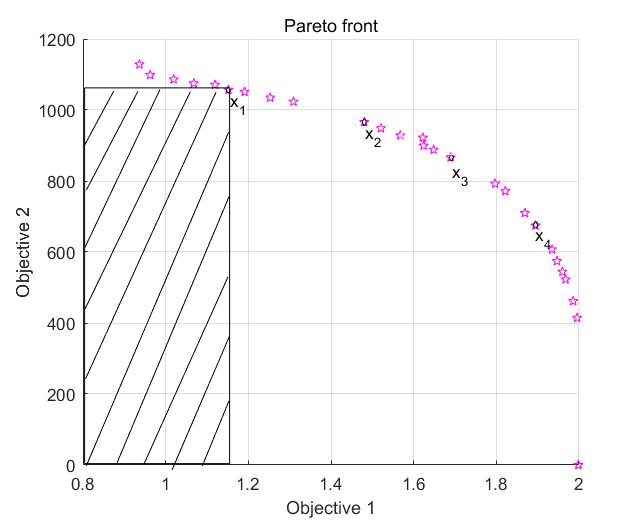
\includegraphics[width = 8cm]{images/pareto_qiandan_exapmle.jpg}
            \caption{二目标规划问题pareto前端示意图}
            \label{二目标规划问题pareto前端示意图}
            \end{figure}
            % \textcolor[rgb]{1.00,0.00,0.00}{todo:图片:二目标规划问题pareto前端示意图}
            \par
            图中$x_1,x_2,x_3,x_4$为Pareto最优解,阴影部分中的解为被$x_1$支配的解,所有Pareto最优解形成Pareto前端。
            \par
            GA在多目标规划问题中的应用始于Schaffer(1985)提出的向量估计遗传算法(UEGA)。多目标进化算法(MOEA)经过了以下三个阶段。
            1) 1985-1994年缓慢发展期:该阶段的算法包括非Pareto方法和Pareto方法。其中,非Pareto方法没有直接使用Pareto最优解的基本概念,具有高效且易实现的特点,但不能产生Pareto最优前端的某些部分(片段)。而Pareto方法则利用劣排序和选择,使整个种群毕竟Pareto最优前端。第一代算法的代表有UEGA、多目标遗传算法(MOGA)、小生境技术(NPGA)和非劣排序遗传算法(NSGA)。2) 1994-2003快速发展期:从1994年Zitzler和Thiele提出强度Pareto进化算法(SPEA)开始,许多研究者开始把外部档案式外部种群结合到多目标进化算法中,精英保留策略成为第二阶段的基本设计步骤。代表算法有NSGA\rom{2}、Pareto档案进化策略(PAES)、Pareto包络选择算法(PESA)以及SPEA2等。3) 2003年至今:从2003年开始,多目标进化算法进入到一个新的阶段,混合策略、并行策略、协同进化策略、动态进化策略和动态多目标优化问题也有初步发展。
            \par
            多目标算法设计的基本要求:\ding{172}提供一组尽可能大的非劣解;\ding{173}要使这组解逼近问题的全局Pareto前端;\ding{174}解集合尽可能均匀分布在整个全局最优前端上。
            \par
            多目标算法的性能指标:世代距离GD、收敛性指标$\gamma$和多样性指标$\Delta$等,主要用来评价所求解与全局Pareto前端的逼近程度和收敛性。下面,我们给出多目标算法的一些性能指标。
            \begin{definition}[收敛性指标]
            设多目标优化问题的Pareto最优集是已知的,在问题的Pareto最优前端上均匀的取一些点(如500个),计算由算法获得的解与这些点之间距离的最小值,所有这些最小值的平均值就是收敛性指标$\gamma$。
            \end{definition}
            \begin{definition}[多样性指标]
            将算法获得的所有非劣解按某个目标函数值的大小有序的分布在目标空间上,$h_i$为相邻两点间距离,$\bar{h}$为$h_i$的均值,$h_f,h_1$分别是算法获得的边界解与相应极端解的距离,则多样性指标$\Delta$为
            \begin{align*}
            \Delta = \frac{h_f - h_1+\sum_{i=1}^{n-1}|h_i - \bar{h}|}{h_f+h_1+(n-1)\bar{h}}
            \end{align*}
            \end{definition}
            \begin{definition}[SP指标]
            指标SP描述非劣解在目标空间上的分布范围
            \begin{align*}
            SP = \sqrt{\frac{1}{n-1}\sum_{i=1}^n(\bar{d}-d_i)^2}
            \end{align*}
            式中,$d_i = \min_{j=1,2,\dots,n}\left( \sum_{k=1}^M|f_k^i - f_k^j| \right) $,$\bar{d} = \frac{1}{n}\sum_{i=1}^nd_i$。
            \end{definition}
            \begin{definition}
            Zitzler等给出了3个用于度量算法求解质量的指标
            \begin{align*}
            & M_1^*(NP) = \frac{1}{|NP|}\sum_{p\in NP}\min\{||\mathbf{p}-\bar{\mathbf{p}}||,\bar{\mathbf{p}}\in P_F\}\\
            & M_2^*(NP) = \frac{1}{NP-1}\sum_{p\in NP} |\{\mathbf{q}\in NP,||\mathbf{q}-\mathbf{p}||^* >\sigma ^*  \}|\\
            & M_3^*(NP) = \sqrt{\sum_{i=1}^M\max\{||p_i-q_i||^*,\mathbf{p},\mathbf{q}\in NP\}}
            \end{align*}
            其中,$NP$为算法获得的非劣解集;$P_F$为问题的Pareto最优前端。
            \end{definition}
            \par
            $M_1^*$确定非劣解集$NP$与$P_F$之间的平均距离。分布性指标$M_2^*$则反映了$\sigma^*$-niches的数量,其值取在区间$[0,|NP|]$内,且其值越大,反应算法获得的非劣解分布越均匀。$M_3^*$测量$NP$中非劣解在Pareto最优前端的分布范围。
            \begin{definition}[误差比ER]
            误差比ER用来描述在算法产生的非劣解中,不属于真实Pareto前端的解所占的百分比
            \begin{align*}
            ER = \frac{\sum_{i=1}^ne_i}{n}
            \end{align*}
            其中:$n$为所获得的非劣解的个数,若解$i$属于Pareto最优解集,则$e_i=0$;否则,$e_i=1$。ER值越小,属于Pareto最优解集的非劣解所在比例越高。$ER=0$表示所在非劣解都位于真实的Pareto前端上。
            \end{definition}
            \begin{definition}[GD距离]
            GD用来描述算法所获得的非劣解与问题的真实Pareto前端之间的距离
            \begin{align*}
            GD = \frac{\sqrt{\sum_{i=1}^n\mathrm{dist}_i^2}}{n}
            \end{align*}
            其中:$\mathrm{dist}_i$表示第$i$个非劣解与真实Pareto前端之间的最短距离。
            \end{definition}
            \par
            多目标算法的测试函数:如果想测试一下设计的多目标算法的求解性能,可以用一些函数来测试。关于多目标算法的测试函数,可以参考网址\footnote{http://www.xuebuyuan.com/2224684.html}。
        \subsubsection{第一代多目标进化算法}
            \par
            由于很多第二代MOEA都是在第一代MOEA的基础上发展起来的,因此,我们先简要介绍第一代多目标进化算法。
            \paragraph{1)向量估计遗传算法(VEGA)}
            VEGA具体的过程如下:设有$p$个目标函数,针对每个目标利用比例选择法,分别产生$p$个子种群,每个子种群的规模为$N/p$。这$p$个子种群分别得到进化后,再将他们合并为一个大小为$N$的种群,再执行遗传操作。重复上述过程,直到收敛。
            \paragraph{2)多目标遗传算法(MOGA)}
            在MOGA中,个体的秩等于当前种群中支配他的染色体数目加1,所有非劣个体的秩均为1(所有这样的个体适应度都相同,以便能以相同的概率别选择使用),而被支配的个体依据属于他们所在区域的种群密度被惩罚(适应度共享用于验证个体区域的拥挤程度)。适应度赋值方式如下:\ding{172}基于个体的秩将种群排序;\ding{173}利用线性或非线性的插值方法在最低序号(非劣最优个体)与最高序号之间进行插值;\ding{174}具有相同序号的个体的适应值共享,即通过除以相同序号的个体数得到新的适应值。可以给不同序号的个体分配固定不变得适应值。
            \par
            MOGA的优点是算法执行相对容易且效率高,缺点是算法易受小生境大小的影响。值得一提的是,Fonseca等已经从理论上解决了小生境大小的计算问题。
            \paragraph{3) 非劣排序遗传算法(NSGA)}
            基于Goldberg的方法,NSGA对个体分类,形成多个层次。具体过程为,在选择操作之前,个体基于Pareto最优进行排序:所有非劣的个体归为一类,并引进决策向量空间的共享函数法,保持种群的多样性;然后,忽略这些已经分类的个体,考虑另一层非劣的个体;这个过程一直持续,直到将所有个体分类。由于最先得到的非劣个体有最大的适应度,他们被复制的机会更多。
            \par
            NSGA的优点是最优目标个数任选,非劣最优解分布均匀,允许存在多个不同等效解;缺点是由于Pareto排序要重复多次,计算效率较低。计算复杂度为$O(MN^3)$,未采用精英保留策略,共享参数$\sigma_{share}$需要预先确定。
            \paragraph{4) 小生境Pareto遗传算法(NPGA)}
            NPGA使用基于Pareto支配的锦标赛选择模式,其基本思想非常巧妙:随机选择两个个体,与来自种群的一个子集比较(典型的,子集占整个种群的$10\%$),若其中一个个体支配自己,而另一个个体被子集支配,则非劣个体获胜;若两个个体都不受或都受子集支配,则采用共享机制来选取其中之一参与下一代进化。因为该算法的非劣解选择是基于种群的部分而非全体,所以其优点是能很快找到一些好的Pareto最优解域,并能维持一个较长的种群更新期。缺点是除了需要设置共享参数外,还需要选择一个适当的锦标赛规模,因而限制了该算法的实际应用效果。
        \subsubsection{第二代多目标进化算法}
            \par
            这一部分,我们将介绍精英策略、共享策略、分级策略以及SPEA、SPEA2、NSGA\rom{2}、IENSGA\rom{2}等多目标进化算法。
            \paragraph{精英策略Elitist srtategy}精英策略就是在算法的迭代过程中,从上一代保留优秀的潜在解至下一代的过程,简单地从上一代中直接拷贝相应的解至下一代是常用的方法。早在1975年,精英策略已经被认为是一种改进EA算法效率的有效手段,当前在多目标优化领域的一些研究也显示该策略能有效改善MOEA算法的效率。对于单目标优化,精英策略的应用是非常简单和显而易见,因为在种群中仅有一个最优个体,对于多目标优化,该策略的使用却要复杂很多。可以定义当前种群的所有非劣的个体的集合为精英解集或称为归档,但是显然,随着运行代数的增加,该解集的个体数量会趋于原种群的个体数量,无改变地拷贝大量的精英进入下一代会妨碍整个种群的进一步进化。
            \par
            可以总结,多目标优化的精英策略面临两个问题:1.怎样控制精英种群的大小;2.怎样使用精英策略更好地指导搜索。Zitzler和Thiele提出了一种简单有效的MOEA精英策略,并在此基础上得到了SPEA算法。该算法的成功使精英策略在MOEA领域得到了新的重视。Deb也于2000年提出了采用精英策略的NSGA\rom{2}算法。简单地可将精英策略划分为两种:在线归档(no-line)和离线归档(off-line)。在线归档和离线归档的区别在于虽然离线归档也在每一代中不断更新,但归档中的精英个体不显式地用于产生下一代。
            \paragraph{共享策略(sharing strategy)}多目标演化算法的目标之一是要在可行区域中获得一个适当分布的候选解集供决策者使用。在演化算法的整个种群中形成各个子种群簇的方法可用来达到这个目的,该类技术也被称为小生境技术。适应值共享是小生境技术的一个较成功的实现,在该方法中,每个候选解的原始适应值需要根据其局部种群密度进行校正。这里所说的局部种群的密度一般是指在可行区域内度量,其直接体现了保持解的较好分布的目标。适应值共享策略较好地解决了gneeticdrfit的问题,避免算法陷入局部最优,使算法更有可能获得一个分布合适的Paerot阵面。
            \paragraph{分级策略(Ranking strategy)}大多数现代的多目标演化算法都是基于Pareot支配的概念的,并且大致可以分为以下的两种具体的分级策略:
            \begin{enumerate}
            \item Non-dominated sorting(NDS)
            \item Multi-objectiv ranking(M0R)
            \end{enumerate}
            \par
            两种方法的思想都非常简单,对于NDS方法,考虑需要比较的候选解集和其对应的目标向量,Goldberg把解集分成不同的非支配层次:初始时,候选解集的全局非支配解被赋予最高的级别,如用0表示,然后将这些非支配解暂时从考虑的解集中移走;考虑剩下的解集中的解,对其中的非支配解又赋予较高的级别,如用1表示,再移去这些非支配解;如此类推,直到剩下的解集为空为止。
            \par
            MOR方法并不产生一系列的非支配阵面,对于每一个个体,仅仅计算在候选的解集中支配它的个体的数量。这样,全局非支配的个体赋予为0的较高的等级,其它个体次之。两种方法都能达到这样的基本目标目的:所有的首选解被赋予相同的等级0;更好的解被赋予更高的等级。不同的现代算法采用不同的方法,例如SPEA算法采用MOR算法,而NSGAZ算法采用NDS算法,没有明显的证据表明哪种算法更优。
            \paragraph{强度Pareto进化算法(SPEA)}SPEA算法使用一个规则群体和一个在线归档。开始时初始化一个种群和一个空的在线归档,以下步骤重复进行。首先,将种群中未被支配的个体成员拷贝到在线归档中;在在线归档中去除任意被支配的个体或者重复个体,如果这个被不断更新的在线归档大小超过了预先定义的大小,那么为了保持未被支配阵面的特征,在在线归档上采用簇方法去除多余的个体成员;然后对在线归档和种群中的成员进行适应值赋值,并将群体和在线归档中的个体通过锦标赛选择再经过杂交和变异替代父代群体成为下一代群体,SPEA算法具体步骤如下:\\
            \textbf{Step1.}产生初始种群$P$和空的外部非劣解集$NP$。\\
            \textbf{Step2.}将种群$P$中的非劣个体拷贝考非劣解集$NP$。\\
            \textbf{Step3.}剔除集合$NP$中受种群$P$中个体支配的解。\\
            \textbf{Step4.}如果保留在集合$NP$中的非劣解的个数超过事先给定的最大值,则通过聚类分析对集合NP进行修剪,提出多余的解。\\
            \textbf{Step5.}计算种群$P$和集合$NP$中的每个个体的适应度值。\\
            \textbf{Step6.}利用二元锦标赛方法从$P\cup NP$中选择个体进入下一代。\\
            \textbf{Step7.}对个体实施交叉和变异操作。\\
            \textbf{Step8.}终止条件。不终止则返回Step2.
            \par
            下面我们详细介绍适应度赋值过程和聚类分析过程。\ding{172}\textbf{适应度赋值}分为两个阶段,首先对非劣解集$NP$中的个体进行赋值,然后对种群中的个体赋值。具体描述如下:(1)对于每个解$x_i\in NP$,赋予一个强度值$s_i\in [0,1)$,$s_i = h_i/(N+1)$,其中$h_i$表示种群中受个体$x_i$支配的个体数,$N$为种群规模。个体$x_i$的适应度值$f_i = s_i$;(2)每个个体$x_j\in P$的适应度值$f_j = 1+\sum\limits_{i,x_i \succ x_j}s_i$,即所有支配解$x_j$的解$x_i\in NP$的强度秩和再加1。
            \par
            \ding{173}\textbf{聚类分析}:通常情况下,非劣解集大小必须受限,必须为其规定最大规模,即保留在其中的解的最大个数,主要原因有4个方面(1)MOP的非劣解集大小可能非常大,甚至是无穷大;(2)实现算法的计算资源是有限的;(3)档案维数的复杂性会随档案规模变大而显著增加;(4)遗传漂移可能出现,因为在均匀采样过程中搜索空间中过度代表的区域总是优先被选择。
            \par
            前三点意味着必须限制档案的大小,而第四点表示对档案进行修剪可能对算法性能有利。SPEA采用如下聚类算法对非劣解集进行修剪:\\
            \textbf{Step1.}初始化聚类集$C$,该集合由非劣解集$NP$的解构成,每个解对应一个聚类。\\
            \textbf{Step2.}如果$|C |\leqslant \bar{N}$,转到Step5;否则转到Step3.\\
            \textbf{Step3.}计算所有聚类之间的距离,两个聚类$c_1,c_2\in C$之间的距离$d=\frac{1}{|c_1||c_2|}\sum\limits_{i_1\in c_1,i_2\in c_2}||i_1-i_2||$,其中$||i_1-i_2||$表示两个个体在目标空间上的欧式距离。\\
            \textbf{Step4.}确定具有最小距离的两个聚类$c_1,c_2\in C$,然后调整聚类集$C = C/\{c_1,c_2\}\cup\{c_1\cup c_2\}$,转到Step2.\\
            \textbf{Step5.}确定每个聚类的代表个体。通常选择和同一聚类的其他个体之间的平均距离最小的个体作为该聚类的代表。其中$\bar{N}$为外部非劣解集的最大大小。
            \paragraph{强度Pareto进化算法2(SPEA2)}在SPEA2算法中,它去除了原有算法的弱点并且加入了一些新的方法,SPEA2算法使用的是细粒度赋值策略,它组合进了密度信息。在这个算法中,每一个解,不论它是Pareto大于还是Pareto小于其他解,表示这个解的个体总是被考虑进来。SPEA2的算法步骤如下:\\
            \textbf{Step1.}产生初始种群$P_0$和空的外部档案$A_0$,令$t:=0$。\\
            \textbf{Step2.}计算种群$P_t$和外部档案$A_t$内个体的适应度值。\\
            \textbf{Step3.}确定$A_{t+1} = \{x_i|x_i\in P_t\cup A_t\text{非劣}\}$,如果$A_{t+1}$的大小超过$\bar{N}$,则修剪$A_{t+1}$;如果$A_{t+1}$的大小小于$\bar{N}$,则将$P_t$和$A_t$中的受支配解加入到$A_{t+1}$中,直到其大小等于$\bar{N}$。\\
            \textbf{Step4.}如果$t>T$,则输出外部档案$A_{t+1}$,并停止搜索。\\
            \textbf{Step5.}对外部档案$A_{t+1}$采用替代的二元锦标赛方法选择个体进入交配池。\\
            \textbf{Step6.}对交配池和种群$P_{t+1}$实施交叉和变异操作,$t=t+1$转到Step2.
            \par
            下面描述适应度赋值和外部档案维护的具体过程。\ding{172}\textbf{适应度赋值}为了避免被同样的外部档案成员支配的个体具有相同的适应度值,在SPEA2中,每个个体的所支配的解和支配它的解都被考虑在内。种群和外部档案中的个体$i$都被赋予一个强度值$S(i)$,表示受该个体支配的解的数量
            \begin{align*}
            S(i) = |\{j|x_j\in P_t+A_t,x_i\succ x_j\}|
            \end{align*}
            在$S(i)$的基础上,个体$i$的原始适应度值$R(i)$等于支配该个体的所有个体的强度值之和,即
            \begin{align*}
            R(i) = \sum_{x_j\in P_t+A_t,x_j \succ x_i} S(j)
            \end{align*}
            与SPEA不同的是,计算$R(i)$时,种群和外部档案内的个体都考虑在内,而且原始适应度值越小,说明支配该个体的个体少,$R(i) = 0$表示个体$i$为非劣解。
            \par
            原始适应度赋值过程提供了一个非劣排序,但仅仅非劣排序还不够,必须引入密度信息以区分具有相同原始适应度值得个体。SPEA2采用$k$近邻方法来计算个体$i$的密度值$D(i)$
            \begin{align*}
            D(i) = \frac{1}{\sigma_i^2+2}
            \end{align*}
            其中:$\sigma_i^2$为个体$i$与第$k$个近邻个体在目标空间上的距离,$k = \sqrt{N+\bar{N}}$。最终,个体$i$的适应度值$F(i)$为原始适应度值和密度值之和
            \begin{align*}
            F(i) = R(i)+D(i)
            \end{align*}
            \ding{173}\textbf{外部档案维护}SPEA2的档案维护过程与SPEA存在两个点差异:(1)档案大小始终是一个常数;(2)档案维护避免了边界解从档案中移出。具体过程如下:\\
            \textbf{Step1.}将种群$P_t$和外部档案$A_t$的所有非劣解拷贝到$A_{t+1}$中,如果$A_{t+1}$的大小刚好等于$\bar{N}$,则接受。\\
            \textbf{Step2.}如果$|A_{t+1} < \bar{N}|$,则将$P_t$和$A_t$最好的$\bar{N} - |A_{t+1}|$个受支配解加入到$A_{t+1}$中。\\
            \textbf{Step3.}如果$|A_{t+1} > \bar{N}|$,则不断的将档案$A_{t+1}$中的解移出直到$|A_{t+1}| = \bar{N}$,在修剪档案过程中,根据如下原则决定哪个解从档案中移出,如果个体$i$满足如下条件则从$A_{t+1}$中剔除。对所有个体$j$,$i<dj$,其中,$i<dj$当且仅当$\forall 0<k<|A_{t+1}|$,有$\sigma_i^k = \sigma_j^k$,或者$\exists 0<k<|A_{t+1}|$,有$\sigma_i^k<\sigma_j^k$,且对$\forall 0<l<k$有$\sigma_i^l = \sigma_j^l$。

            \paragraph{NSGA\rom{2}}Deb.et和他的学生们于2000年提出了一种精英策略的非劣分类遗传算法NSGA\rom{2}。在大多数方面,该算法与初始的NSGA没有太多的相似性,创始者为了强调它的起源而保持了NSGA\rom{2}这个名字。
            \par
            在NSGA\rom{2}中,首先用亲代种群$P_n$产生子代种群$Q_n$,并将两个种群联合在一起形成大小为$2N$的种群$R_n$。然后使用非劣分类将整个种群$R_n$分等级。尽管与只对$Q_n$进行非劣分类相比,它需要做更多的工作,但是它允许在整个子代和亲代进行全局的非劣检验。一旦结束非劣分类,新种群$P_{t+1}$由不同的非劣等级的个体填充。填充过程从最优非劣等级开始,接着是第二非劣等级,依此类推。由于整个种群凡的种群大小为$2N$,新种群的$N$个位置不能容纳所有的非劣等级。当考虑被允许的最后一等级中的解时,该非劣等级可能存在比新种群剩下位置更多的个体。在这种情况下,使用密度估计的方法从最后一等级选择位于该等级较稀疏区域的个体填充满该种群。这里着重要指出的是$R_n$的非劣分类过程和种群$P_{n+1}$的填充过程可以一起执行。这样,每次找到一个非劣等级并检查它的大小,看它是否能被新种群容纳,如果不能,那么就不必再进行非劣分类,这样能减少该算法的运行时间。NSGA\rom{2}的具体过程描述如下:\\
            \textbf{Step1.}随机生成初始种群$P_0$,然后对种群进行\underline{非劣排序},每个个体被赋予秩;再对初始种群执行二元锦标赛选择、交叉和变异,得到新种群$Q_0$,令$t=0$。\\
            \textbf{Step2.}形成新的群体$R_t  = P_t\cup Q_t$,对种群$R_t$进行\underline{非劣排序},得到非劣前端$F_1,F_2,\cdots$。\\
            \textbf{Step3.}拥挤度选择操作。对所有$F_i$按排挤比较操作$\prec_n$进行排序,并选择其中最好的$N$个个体形成种群$P_{t+1}$。\\
            \textbf{Step4.}对种群$P_{t+1}$进行复制、交叉和变异,形成种群$Q_{t+1}$。\\
            \textbf{Step5.}终止条件。不终止,则$t:=t+1$返回Step2.
            \par
            下面介绍上述算法中所使用的快速非劣分类方法、拥挤距离尺度以及拥挤选择算子。
            (一)快速非劣分类方法:首先,对于每一个解我们计算两个量:\ding{172}支配解$i$的解的个数$n_i$;\ding{173}$i$支配的一组解$S_i$。这两个量的计算时间为$O(MN^2)$。随后,将所有$n_i=0$的解放入解集$F_1$中。对于当前解集$F_1$中的解$i$,观察它的$S_i$集,将$S_i$集中每个解$j$的$n_j$数减1,作完上述步骤后,如果支配$j$的解个数$n_j=0$,这也就意味着$j$是仅次于第一等级中解的个体。此时把$j$放入$F_2$中。重复上述过程,最终将所有的解按照非劣关系分为多个等级。其中$F_1$中的解是最好的,也就是前面所提到的精英解,它只支配解而不被其他任何解支配,凡中的解只被$F_1$中的解支配,不被其它解支配,依次类推。
            \par
            每次迭代时间为$O(N)$,由于最多有$N$个解集,那么最坏情况下这个循环的时间为$O(N^2)$。总时间复杂度为$O(MN^2)+O(N^2)$或者$O(MN^2)$。
            \par
            (二)拥挤距离:种群中某个个体$i$的拥挤距离$d_i$是一个在个体$i$周围不被种群中任何其它的个体所占有的搜索空间的度量。为了估计种群中某个个体$i$周围个体的密度,取个体$i$沿着每个目标的两边的两个个体$(i-1),(i+1)$的水平距离,数量$d_i$作为$M$个距离之和的估计值,称之为拥挤距离。拥挤度距离的求解步骤为(1)每个点的拥挤距离$d_i$设置为0;(2)设$f_m$为目标函数$m=0,1,\dots,M$,设$d_0 = d_l =\infty $,并且对其他所有个体$i = 1,2,\dots,l-1$,分配
            \begin{align*}
            d_i = \sum_{m=0}^M \left( |f_m^{i+1} - f_m^{i-1}| \right)
            \end{align*}
            其中:$d_i$表示第$i$个点的拥挤距离,$f_m^{i+1}$表示第$i+1$个点的第$m$个目标函数值。
            \par
            (三)拥挤选择算子:在NSGA\rom{2}中,定义拥挤比较算子$\prec_n$如下
            \begin{align*}
            & if(i_{rank}<j_{rank})or((i_{rank} = j_{rank})and(i_{diatance}>j_{diatance}))\\
             \Rightarrow {} & i\prec_n j\quad (\text{解i优于解j})
            \end{align*}
            它假设每个个体$i$有两个属性:1.种群中的非劣等级$r_i$;2.种群中的局部拥挤距离$d_i$。依据这两个属性,可以定义拥挤度选择算子如下
            \begin{definition}[拥挤选择算子]
            个体$i$与另一个个体$j$进行比较,只要下面任意义个条件成立,则个体$i$获胜:1.如果个体$i$所处等级优于个体$j$所处等级,即$r_i<r_j$;2.如果他们有相同的等级,且个体$i$比个体$j$有一个更大的拥挤距离,即$r_i=r_j\ \& \ d_i>d_j$。
            \end{definition}
            \par
            第一个条件确保被选择的个体属于较优的非劣等级。第二个条件根据它们的拥挤距离选择由于在同一非劣等级而不分胜负的两个个体中位于较不拥挤区域的个体(有较大的拥挤距离$d_i$)。在联赛选择和新种群填充阶段都使用了拥挤比较过程,通过使用拥挤比较过程引入了非劣解集内个体的多样性分布。由于个体通过它们的拥挤距离(邻近个体密度度量)来竞争,因此,这里不需要专门的小生境参数(例如在MOGAs、NSGAs或NPGAs中需要的参数$\sigma_{share}$)。尽管是在目标函数空间计算拥挤距离,但是,如果需要的话,也能在参数空间实现拥挤距离的计算。
            \paragraph{IENSGA\rom{2}}在试验过程中,我们发现NSGA\rom{2}算法仍然有一定的缺陷:保留精英也就意味着强调子代中的最优解。在许多情况下,一个种群主要由当前最好的非支配解组成,那么,这些解都是精英,当前种群也就不能再接纳一些新的解参与下一代的操作,搜索过程将中止并过早的收敛到局部的Pareto解。在NSGA\rom{2}中,由于没有限制精英解的范围,使得NSGA\rom{2}在六个测试问题(ZDTI,ZDTZ,ZDT3,ZDTI4,ZDT6,KUR)上的仿真结果显示大概在20代以后,种群中的所有解都是精英,随后各代的操作都将在精英解中进行,非精英解无法参与其中,降低了解的多样性。由于精英操作导致绝大多数的非精英解不能参与遗传操作,使得全局解的搜索速度减慢并最终导致种群过早收敛到局部Pareto解。为了确保搜索向全局Pareto优解收敛,一种确保解的多样性的改进的精英策略被提出,在改进精英策略方面我将重点放在了控制精英范围上,取得了很好的效果。将这种改进精英策略(ImporvedElitist)的NSGA\rom{2}算法称为IENSGA\rom{2}。
            \par
            在改进的算法中,我们的目标是确保个体的多样性从而得到较好的收敛性。因此,自适应的限制当前精英解集的范围从而使非精英解集也能平等的参与到新种群的操作就显得尤为重要。分布函数如下
            \begin{align}
            \label{IENSGA2的分布函数}
            n_i = N\frac{1-r}{1-\sin(r^m)}/(\sin r)^i+share
            \end{align}
            其中:$n_i(m \leqslant i \leqslant 1)$是当权等级中允许的最大个体数,$i$是当前种群级别,$N$是种群规模,$m$是当前种群(合并后的规模为$2N$的种群)中非劣等级的数目,$r(0<r<1)$是一个可以由用户来自定义的参数。IENSGA\rom{2}的算法流程如下:\\
            \textbf{Step1.}对种群$R_t = P_t \cup Q_t$进行快速非支配排序,并对每个个体计算拥挤距离。\\
            \textbf{Step2.}根据公式(\ref{IENSGA2的分布函数}),计算出每个等级中所允许的最大个体数目,由于$r<1$,因此等级1$(i=1)$中允许的个体数是最多的,而等级1中的解是当前种群中最好的非劣解,也就是所谓的精英解。这充分照顾到了精英解,使得较多的精英解参与遗传操作中。由公式不难看出,随着等级数即$i$值的增大,各个等级中所允许的个体数目依次减少,这对于各个等级都是公平的,也体现了“适者生存,优胜劣汰”的思想。\\
            \textbf{Step3.}与NSGA\rom{2}类似,按照第二步的方法将$N$个符合条件的解放入下一代中,继续对其执行选择、交叉、变异等遗传操作。


        \subsubsection{多目标混合进化算法}
            \par
            防止过早收敛的有效方法之一是进化算法与局部搜索混合,这样的混合算法叫memetic算法。Ishibuchi等最早于1998年提出了多目标遗传局部搜索(MOGLS),记为IM-MOGLS。Ishibuchi等于2003年修改了IM-MOGLS的局部搜索过程,得到IM-MOGLS2。在简单MOGLS(S-MOGLS)中,遗传搜索和局部搜索之间有四种可能组合,遗传搜索可能根据标量适应度值或根据Pareto排序与拥挤距离选择父代个体,而局部搜索可能根据Pareto ranking或标量适应度值决定是否接受新解。
            \par
            Jaszkiewicz设计一种MOGLS:J-MOGLS,在每一次迭代中,算法随机确定一个效用函数,然后构造一个临时种群,该种群包含很多选定的效用函数值最好的解,然后从临时种群中选出一对个体进行重组,局部搜索作用于重组得到的新解。Talbi等提出了一种简化的遗传局部搜索,该算法先用遗传算法搜索,GA停止后,再应用多目标局部搜索。在Arroyo等提出的AA-MOGLS中,精英策略、保持种群多样性以及并行多目标局部搜索被引入到MOEA中。
            \par
            M-PAES是在局部搜索多目标优化算法(1+1)PAES基础上建立起来的。在M-PAES中存在两个档案:全局档案G和局部档案H,全局档案为非劣解的有限集,局部档案作为比较集用在局部搜索阶段即(1+1)PAES中。雷德明等利用混沌现象的内在特性,将混沌搜索引入到MOEA中,在每一代,当种群完成一次进化(复制、交叉和变异)之后,在外部档案的部分个体附近进行混沌搜索以产生更多非劣解,引导MOEA新的进化。郭秀萍等将基于加权函数的局部搜索和基于Pareto支配关系的交叉、变异和网格微扰动算法相结合,提出了一种混合自适应多目标memetic算法。
            \paragraph{多目标遗传局部搜索:IM-MOGLS}
            在IM-MOGLS中,具有随机权值的标量适应度函数用于父代种群的选择和局部搜索,遗传搜索产生的种群的每个个体都参与局部搜索,当不能从当前解的领域中随机选择的$k$个领域解中找到更好的解时,局部搜索中止。IM-MOGLS具体描述如下:\\
            \textbf{Step1.}初始化。\\
            \textbf{Step2.}计算当前种群中每个个体对应的目标向量,并对临时非劣解进行升级。\\
            \textbf{Step3.}选择:重复执行如下过程选择$N-N_{elite}$对父代个体。
            \par
            \ding{172}随机确定各目标函数权值$w_i=rand_i/{\mathop{\sum}\limits_{j=1}^Mrand_j}$。
            \par
            \ding{173}根据选择概率选择一对父代个体。\\
            \textbf{Step4.}交叉和变异,对$N-N_{elite}$对父代个体的每对执行交叉操作,每队父代个体通过交叉产生一个新个体,然后对新个体执行变异操作。\\
            \textbf{Step5.}从临时非劣解集中随机选出$N_{elite}$个个体与前面产生的$N-N_{elite}$个个体一起构成新的群体。\\
            \textbf{Step6.}对群体中的所有解进行局部搜索,局部搜索方向由Step3父代个体选择时确定的权值决定,并用局部搜索产生的$N$新解替代当前种群。\\
            \textbf{Step7.}若终止条件成立,结束;否则转到Step2。
            \par
            上述算法中,$N$为种群规模,$N_{elite}$为精英个体数,每个个体的选择概率为
                \begin{align}
                  p(x) = \frac{f(x)-f_{\min}}{\mathop{\sum}\limits_{x\in P}\{f(x)-f_{\min}\}}
                \end{align}
            其中,$f_{\min}$为种群$P$中最劣个体的适应度值,$f_{\min}=\min\{f(x)|x\in P\}$。
            \par
            在Step3中,各个目标函数的取值随机确定,每一组权值都将对应一种搜索方向。因此,局部搜索的方向是多样的。
            % 如图(\ref{fig:IM-MOGLS中的各种搜索方向})所示
            %    \begin{figure}[H]
            %      \centering
            %      \includegraphics[height=4cm]{images/IMMOGLS_search_direction.jpg}
            %      \caption{IM-MOGLS中的各种搜索方向}
            %      \label{fig:IM-MOGLS中的各种搜索方向}
            %    \end{figure}
            \par
            混合算法对新群体中的每个解进行局部搜索,局部搜索具体过程如下:\\
            \textbf{Step1.}确定一个初始解$x$。\\
            \textbf{Step2.}产生当前解$x$的邻域解$y$。\\
            \textbf{Step3.}如果$y$优于当前解$x$,则取代之。\\
            \textbf{Step4.}如果当前解$x$的随机选择的$k$个邻域解都不能优于当前解,则结束;否则转到Step2。
            \par
            当当前解的$k$个邻域解都不能优于当前解时,算法结束。$k$太小,局部搜索会很快结束;$k$太大,局部搜索过程将很大。
            \par
            IM-MOGLS包含两个解集:当前种群和临时非劣解集。局部搜索完毕后,当前种群被局部搜索产生的新解替代,同时临时非劣解集也得到了更新,即将不受当前种群中其他个体和临时非劣集中的个体支配的种群个体加入到临时集中,同时剔除临时解集中的受支配解
            % ,如图(\ref{fig:临时非劣解集的更新过程})所示。
            局部搜索的部分初始解来自临时非劣解集,非劣解的局部搜索方向由其父代个体选择时所使用的权值决定,如果非劣解没有父代如非劣解为非劣解为随机产生的初始解,则随机产生一个搜索方向。
            %    \begin{figure}[H]
            %      \centering
            %      \includegraphics[height=4cm]{images/temporary_noninferior_update.jpg}
            %      \caption{临时非劣解集的更新过程}
            %      \label{fig:临时非劣解集的更新过程}
            %    \end{figure}
            \paragraph{多目标遗传局部搜索:IM-MOGLS2}
            Ishibuchi等修改了IM-MOGLS的局部搜索过程,为每个被选中的解的拷贝确定了固定的局部搜索概率,而且只有锦标赛选择过程中获胜的个体才能作为局部搜索的初始解,并为每个初始解规定了合适的局部搜索方向。为描述方便,记为IM-MOGLS2,计算结果表明,IM-MOGLS2性能明显优于IM-MOGLS。
            \par
            IM-MOGLS2与IM-MOGLS的唯一差别在于Step6,即局部搜索过程。改进过程如下:
            \par
            重复如下三步骤$N$次,然后用这$N$个解去替代当前种群。
            \par
            \textbf{Step1.}随机确定权值$w_1,w_2,\cdots,w_M$,其中,$w_i\ge 0,i=1,2,\cdots,M,\mathop{\sum}\limits_{i=1}^Mw_i=1$。
            \par
            \textbf{Step2.}利用根据Step1的权值而得到的标量函数,使用带放回的锦标赛选择策略,从当前种群中选中一个解,对其进行拷贝后,将其放回种群。
            \par
            \textbf{Step3.}利用现有权值,根据局部搜索概率$p_{LS}$,对选中解的拷贝实施局部搜索。局部搜索的具体过程与原始MOGLS的相应过程相同。如果局部搜索得到实施,将最终得到的解加入另一个种群中;如果局部搜索没有进行,则将拷贝加入到另一个种群中。
            \par
            上述局部搜索的基本思想是尽量不为每个解规定一个适合的局部搜索方向,而是为随机确定的局部搜索方向选择一个适合的解;而且,不对所有选中的解进行局部搜索。使用局部搜索概率的目的在于减少局部搜索的解的个数。
            \paragraph{S-MOGLS}
            S-MOGLS中,遗传搜索和局部搜索之间存在四种可能组合,具体步骤如下:\\
            \textbf{Step1.}随机产生具有$N$个解的初始种群。\\
            \textbf{Step2.}遗传搜索。重新执行如下三个步骤$N$次以产生子代种群:
            \par
            \ding{172}随机确定一个权值向量;
            \par
            \ding{173}利用根据步骤\ding{172}的权值而得到的标量函数使用锦标赛选择策略,从种群中选中一对父代个体;
            \par
            \ding{174}对选出的父代个体进行交叉和变异,以产生一个子代个体。\\
            \textbf{Step3.}局部搜索。通过循环执行如下三个步骤$N$次以得到改进后的种群;
            \par
            \ding{172}随机确定一组权值;
            \par
            \ding{173}利用根据步骤\ding{172}的权值而得到的标量函数,使用锦标赛选择策略,子代种群中选中局部搜索的一个初始解;
            \par
            \ding{174}利用现有权值,根据局部搜索概率$P_{LS}$进行局部搜索,与修改MOGLS不同,只有当初始解通过局部搜索得到改进,局部搜索的最终解才加入到改进后的种群中。\\
            \textbf{Step4.}采用与NSGA2相同的非劣排序过程,从父代种群、子代种群和改进后的种群中选择个体,构成下一代父代种群。\\
            \textbf{Step5.}如果终止条件成立,则停止搜索;否则转到Step2。
            \par
            当遗传搜索和局部搜索使用不同方法进行选择操作时,可以得到S-MOGLS的不同变形,例如遗传搜索和局部搜索都利用标量适应度函数选择个体,或遗传搜索根据Pareto排序结果,而局部搜索根据标量函数选择个体等。实验结果表明,局部搜索和遗传搜索之间的平衡对混合算法的性能有很大的影响;而且,S-MOGLS的不同变形的选择压力不同,但局部搜索初始解的高选择压力对S-MOGLS的性能改善有利。
            \paragraph{J-MOGLS}
            关于MOGLS,除了Ishibuchi等系列工作之外,还有J-MOGLS和AA-MOGLS等算法。下面详细介绍J-MOGLS,先定义效用函数,然后描述算法流程。
            \par
            效用函数$u:{R}^M\to R$将目标空间映射为效用值,它描述决策者的偏好。考虑如下两种两种效用函数。
            \begin{definition}[加权Tchebycheff效用函数]
            加权Tchebycheff效用函数定义如下:
            \begin{align}
              u_{\infty}(y,y^{*},\Lambda) = -\mathop{\max}\limits_{j}\{{\lambda}_j(f_j^*-f_j)\}
            \end{align}
            其中,$\Lambda=\{{\lambda}_1,{\lambda}_2,\cdots,{\lambda}_M\}$,$\forall j,{\lambda}_j\ge 0$为权向量;$y^*=\{f_1^*,f_2^*,\cdots,f_M^*\}$,$f_j^*={\max}\{f_j|y\in Y\},j=1,2,\cdots,M;y=(f_1,f_2,\cdots,f_M)$。
            \end{definition}
            \par
            上述效用函数至少有一个全局最优解是Pareto最优解。对于每个Pareto最优解$x$,存在一个加权Tchebycheff效用函数$u$,使$x$为$u$的全局最优解。
            \begin{definition}[加权线性效用函数]
            加权线性效用函数定义如下:
                \begin{align*}
                  u_{1}(y,\Lambda) = -\mathop{\sum}\limits_{j=1}^M{\lambda}_jf_j
                \end{align*}
            \end{definition}
            \par
            如果存在一组非负权值$\Lambda=\{{\lambda}_1,{\lambda}_2,\cdots,{\lambda}_M\}$,使$x$如下最大化问题的唯一全局最优解:
            \begin{align*}
              & {\max}\ u_{1}(y,\Lambda)\\\notag
              & s.t.\quad x\in D
            \end{align*}
            则$x$为Pareto最优解。
            \par
            由于加权Tchebycheff或加权线性效用函数在Pareto最优解达到最优,J-MOGLS将多目标优化算法的目的转化为寻找所有加权Tchebycheff或加权线性效用函数的最优解。它通过选取效用函数来实现所有效用函数的同时优化,即改善每次迭代时随机选取的效用函数的值来实现。具体描述如下:\\
            \textbf{Step1.}初始化:令非劣解集NP为空,当前解集CS为空。\\
            \textbf{Step2.}重复如下过程$N$次:
            \par
            \ding{172}随机取效用函数$u$,随机构造一个新的可行解$x$;
            \par
            \ding{173}以效用函数$u$为目标,对$x$进行局部搜索,得到$\bar{x}$;
            \par
            \ding{174}对$\bar{x}$加入到当前解集CS中并利用$\bar{x}$更新NP。\\
            \textbf{Step3.}随机选取效用函数$u$。\\
            \textbf{Step4.}从CS中选取$K$个不同解,根据效用函数$u$,这些解最佳;然后由这些解构成临时种群TP。\\
            \textbf{Step5.}随机地从TP中选取两个解$x_1$和$x_2$。\\
            \textbf{Step6.}重组$x_1$和$x_2$,得到解$x_3$。\\
            \textbf{Step7.}以效用函数$u$为目标,对$x_3$进行局部搜索,得到$\bar{x}$。\\
            \textbf{Step8.}如果${\bar{x}}_3$优于TP中的最差解且在决策空间上${\bar{x}}_3$与TP中的任意解不同,则将${\bar{x}}_3$加入到当前解集CS。\\
            \textbf{Step9.}利用${\bar{x}}_3$对集合NP进行更新。\\
            \textbf{Step10.}如果终止条件成立,则停止搜索;否则转到Step3。
            \par
            所谓归一化权值向量指所有非负权值的和为1。在J-MOGLS的每一次迭代过程中,都必须随机选取效用函数,也就是要随机选取如下归一化加权向量:
            \begin{align*}
              {\lambda}_1=1-\sqrt[M-1]{\mathrm{rand}()},{\lambda}_j=\left(1-\mathop{\sum}\limits_{l=1}^{j-1}{\lambda}_l\right)(1-\sqrt[M-1-j]{\mathrm{rand}()}),\cdots,{\lambda}_M=1-\mathop{\sum}\limits_{l=1}^{M-1}{\lambda}_l
            \end{align*}
            其中,$\mathrm{rand}()$为区间$[0,1]$上均匀分布的随机数。
            \par
            为了降低计算量,只利用局部搜索产生的解对NP进行更新和升级,具体步骤如下:如果NP中没有支配${\bar{x}}_3$,则将${\bar{x}}_3$加入到NP中,同时剔除NP中所有受${\bar{x}}_3$支配的解。
            \paragraph{M-PAES}
            M-PAES是在局部搜索多目标优化算法(1+1)PAES基础上,通过利用种群和周期性利用交叉对PAES获得的不同局部最优解进行组合等过程,而建立起来的。M-PAES的建档过程比PAES复杂一些。回顾PAES的算法流程,可以发现,PAES的核心是如何维护一个由有限个非劣解组成且其所能保留的非劣解最大数固定的档案,档案成员是算法搜索过程获得的最好非劣解的代表。(1+1)PAES的档案用于如下两个目标:记录搜索过程中获得的解;用作比较集以确定新的候选解的支配秩。为了在M-PAES中实现上述两个目的,需要两个档案:全局档案G和局部档案H,全局档案为非劣解的有限集,局部档案作为比较集用在局部搜索阶段即(1+1)PAES中。每次局部搜索开始时,H被清空,并从G中选择不能支配候选解$c$的部分解,然后用在(1+1)PAES中以改进$c$;而G在整个搜索过程中得到连续不断地升级和更新。M-PAES具体过程如下:\\
            \textbf{Step1.}随机产生规模为$N$的初始种群$P$并将$P$中所有非劣解加入到全局档案$G$中。\\
            \textbf{Step2.}对于种群$P$中的每个候选解$c$,执行如下过程:\par
            \ding{172}设置当前局部档案$H={\Omega}$(空集);
            \par
            \ding{173}将全局档案$G$中所有不能支配$c$的个体加入到$H$中,同时也将$c$加入到$H$中;
            \par
            \ding{174}执行局部搜索过程PAES(c,G,H),并将改进后的解$c$放回种群$P$。\\
            \textbf{Step3.}设置种群为空:$n_i=0,P_1={\Omega}$。\\
            \textbf{Step4.}执行如下重组过程:
            \par
            \ding{172}令重组次数$r=0$;
            \par
            \ding{173}从$P\cup G$随机选择两个父代个体,然后通过重组产生子代$c$;
            \par
            \ding{174}将$c$与$G$中个体进行比较,如果必要的话,利用$c$更新$G$;
            \par
            \ding{175}$r=r+1$,如果$c$被$G$支配或者$c$位于比两个父代更拥挤的区域且$r < \mathrm{recomb\_trial\_max}$,则转到\ding{173};否则,转到\ding{176};
            \par
            \ding{176}如果$c$被$G$支配,则丢弃$c$并利用二元锦标赛方法从$G$中选择一个新的$c$;
            \par
            \ding{177}将$c$加入到中间种群$P_1$中,$n_i=n_i+1$;
            \par
            \ding{178}如果$n_i < N$,则转到\ding{172};否则,转到Step5。\\
            \textbf{Step5.}利用中间种群$P_1$替代种群$P$。\\
            \textbf{Step6.}如果终止条件成立,则结束;否则,转到Step2。
            \par
            上述算法中,$\mathrm{recomb\_trial\_max}$为最大重组次数,PAES(c,G,H)与(1+1)PAES类似,只是终止条件不同。\\
            PAES(c,G,H)具体描述如下:\\
            $\#fails=0,\#moves=0$;\\
            while$(\#fails<l\_fails,\#moves<l\_opt)$\par
            对$c$进行变异,得到解$x$并计算$x$对应的目标函数值;\par
            $\mathrm{if}\ c \succ x$\par
            \qquad 丢弃$x$;\par
            \qquad $\#fails=\#fails+1$;\par
            $\mathrm{else\ if}\ x\succ c$\par
            \qquad 利用$x$替代$c$;\par
            \qquad 并将$x$加入到局部档案$H$;\par
            \qquad $\# fails=0$;\par
            $\mathrm{else\ if}\quad x$受$H$中任意一个成员支配,丢弃$x$;\par
            $\mathrm{else}$\quad 应用test(c,x,H)以决定$c$和$x$谁成为新的当前解以及是否将$x$加入到$H$中;\par
            $\mathrm{else\ if}$\par
            利用$x$对全局档案$G$进行维护;\par
            $\#moves=\#moves+1$;\\
            end \ while\\
            其中,$l\_opt$为全局搜索最大次数,$l\_fails$为局部搜索失败的最大次数。test(c,x,H)与(1+1)PAES中的test(c,d,A)一样。
            % \paragraph{多目标混沌进化算法}
            % 混沌是非线性系统中的普遍现象,它对进化算法的应用包括建立基于混沌优化的遗传算子、利用混沌搜索不断产生更优的最优个体以引导种群进化以及在算法中利用混沌序列替代随机序列。雷德明利用混沌变量在适应度值最大的几个个体附近搜索新的最优个体,引导种群进化。Determan等设计了基于Logistic函数的变异算子以增强算法的利用能力。Caponetto等研究了在算法中混沌序列完全代替随机数发生器后进化算法性能的改善程度。Li等利用混沌序列动态地增加种群规模以避免过早收敛,目前相关研究不多,雷德明等利用混沌现象的内在特性,将混沌搜索引入到MOEA中,在每一代,当种群完成一次进化(复制、交叉和变异)之后,在外部档案的部分个体附近进行混沌搜索以产生更多非劣解。
            % 多目标混沌进化算法(multi-objective chaotic evolutionary algorithm,MCEA)与大多数MOEA结构相似,只是要将混沌搜索插入其中。MCEA具体步骤如下:\\
            % \textbf{Step1.}产生初始种群并将其中的非劣解拷贝到外部档案中。\\
            % \textbf{Step2.}从种群和外部档案中选择个体进入下一代。\\
            % \textbf{Step3.}执行交叉、变异操作。\\
            % \textbf{Step4.}计算种群中个体对应的目标函数向量并维护档案。\\
            % \textbf{Step5.}从外部档案中随机选择几个个体,分别以这些个体的拷贝作为初始解,进行混沌搜索并根据搜索产生的非劣解进行档案维护。\\
            % \textbf{Step6.}如果满足终止条件,停止搜索;否则转到Step2。\\
            % 下面介绍混沌搜索的具体过程。
            % \par
            % 混沌优化利用混沌变量的随机性、遍历性等内在特性,它的基本思想是把混沌变量线性映射到优化变量的取值区间,然后利用混沌变量进行搜索。混沌优化本质上还是一种局部搜索方法,它必须在搜索过程中不断缩小优化变量的搜索区间,不然算法很难获得最优解。在混沌优化中,最常用的混沌映射为Logistic映射:
            %     \begin{align}
            %       u_{k+1} = \alpha u_k(1+u_k),\quad k=0,1,2\cdots
            %     \end{align}
            % 其中:$u_0 < 1$,当$\alpha = 4$,Logistic系统处于完全混沌状态。
            % \par
            % 当混沌优化与MOEA结合时,仅从外部档案中随机选择几个解,以这些解的拷贝作为混沌搜索的初始解,在它们所在的附近区域搜索新的非劣解。由于只是档案个体的拷贝参与混沌搜索,没有档案个体从档案中移出。混沌搜索产生的非劣解进入外部档案,并根据MOEA的相应方法对档案进行维护。
            % \par
            % 混沌搜索具体步骤如下:\\
            % \textbf{Step1.}设定$u_{0j},j=1,2,\cdots ,n$,$k=0$,$p_{cs}$,$n_{cs}$,cm,$h=1$。\\
            % \textbf{Step2.}对每个决策变量确定$[{\theta}_j,{\beta}_j]$,其中,${\theta}_j=\mathop{\min}\limits_{x\in P\cup \mathrm{NP}}\{x_j\}$,${\beta}_j=\mathop{\max}\limits_{x\in P\cup \mathrm{NP}}\{x_j\}$,如果${\theta}_j-0.1|{\theta}_j|\le w_j$,则${\theta}_j=w_j$,否则${\theta}_j\leftarrow {\theta}_j-0.1|{\theta}_j|$;如果${\beta}_j+0.1|{\beta}_j|\ge \xi_j$,则${\beta}_j=\xi_j$,否则${\beta}_j\leftarrow {\beta}_j+0.1|{\beta}_j|$。\\
            % \textbf{Step3.}随机地从档案中选择一个解,对其拷贝$x^h=(x_{h1},x_{h2},\cdots,x_{hn})$,$v=1$。\par
            % \ding{172}对每个$x_{hj}(j=1,2,\cdots,n)$,产生一个$[0,1]$区间均匀分布随机数$s$,若$s < p_{cs}$,则$y_{hj}\leftarrow x_{hj}+c_ju_{kj}-d_j$;否则$y_{hj}\leftarrow x_{hj}$。\par
            % \ding{173}计算新解$y_v=(y_{h1},y_{h2},\cdots,y_{hn})$对应的目标函数向量,如果它不被种群和档案中的任何解支配,将其保留在集合$\Psi$中,$k\leftarrow k+1$,$v\leftarrow v+1$。若$v < \mathrm{cm}$,转到\ding{172};否则,转到Step4。\\
            % \textbf{Step4.}如果解集$\Psi$中所有非劣解不能支配档案中的任何个体,将$\Psi$中一个非劣解加入到档案中并进行档案维护;否则,对于$\Psi$中的每个非劣解,若它支配了档案中的部分解,让它替代档案中的那些受其支配的个体。\\
            % \textbf{Step5.}$h\leftarrow h+1$,若$h < n_{cs}$,则清空集合$\Psi$并转到Step3;否则,停止搜索。
            % \par
            % 上述算法中,$u_{kj},j=1,2,\cdots,n$是对应于第$j$个决策变量的Logistic混沌变量,$u_{0j}$为其对应的初始值,$p_{cs}$是每个决策变量的混沌搜索概率,而$\mathrm{cm}$则是每个被选中的档案个体的拷贝进行混沌搜索的最大次数。$n_{cs}$为档案中被选中的解的个数。$[w_j,\xi_j]$为第$j$个决策变量的定义域。$c_j,d_j$按如下原则确定以确保每个决策变量在区间$[{\theta}_j,{\beta}_j]$内变化:
            % \par
            % 对于$x_{hj}\in [{\theta}_j,{\beta}_j]$,若${\beta}_j-x_{hj} > {\zeta}_j$,则$\tau_1=\zeta_j$;否则$\tau_1={\beta}_j-x_{hj}$。若$x_{hj}-{\theta}_j > {\zeta}_j$,则$\tau_2={\zeta}_j$;否则$\tau_1=x_{hj}-{\theta}_j$。最终$c_j={\tau}_1+{\tau}_2$,$d_j={\tau}_2$,$\zeta_j,j=1,2,\cdots,n$为小正数。
            % \par
            % 混沌搜索产生的大多数解难以成为外部档案的成员除非它们支配档案内的个体,这样可以避免档案中的解过于相似,因为混沌搜索仅改变档案个体的拷贝的部分基因位,并且变化幅度比较小。

        \subsubsection{MATLAB应用实例}
            \par
            MATLAB中使用gamultiobj命令来求解多目标优化问题,下面给出gamultiobj的命令格式及其示例。gamultiobj可用于求解平滑或非平滑的优化问题,不需要函数可微或连续。它可以创建均匀、可行的初始种群;适应度尺度变换有:基于等级、比例、顶部、线性定标、移位;选择方法有:锦标赛(Tournament);交叉方法有:scatterd(分散)、sigle(单点)、intermediate(中间)、Heuristic(启发式)、arithmetic(算术)、两点;变异方法为:adaptic feasible(自适应可行)、uniform(均匀)、gausian(高斯);可以绘制:平均Pareto距离、平均Pareto散布度、个体间距、个体多样性、个体预期、Pareto front、等级柱状图、选择指数和终止条件。此外,我们还可以指定:群体大小、交叉片段、Pareto片段、个体间的距离测量、子群体迁移、边界约束和线性非线性约束。优化变量可以是整数、混合整数、分类型数和复数。gamultiobj的应用实例如下
            \begin{lstlisting}[language = Matlab]
            %% 1、简单的多目标优化问题
            % min y
            %   y(1) = (x+2)^2 - 10;
            %   y(2) = (x-2)^2 + 20;
            % subject to  -1.5 <= x <= 0

            % Plot two objective functions on the same axis
            x = -10:0.5:10;
            f1 = (x+2).^2 - 10;
            f2 = (x-2).^2 + 20;
            plot(x,f1);hold on;plot(x,f2,'r');grid on;
            title('Plot of objectives ''(x+2)^2 - 10'' and ''(x-2)^2 + 20''');
            %Minimizing Using gamultiobj
            FitnessFunction = @(x)((x+2)^2 - 10;(x-2)^2 + 20);
            numberOfVariables = 1;
            A = []; b = [];
            Aeq = []; beq = [];
            lb = -1.5;
            ub = 0;
            options = gaoptimset('PlotFcns',{@gaplotpareto,@gaplotscorediversity});
            [x,Fval,exitFlag,Output,Population,Score] = gamultiobj(FitnessFunction,numberOfVariables,A,b,Aeq,beq,lb,ub,options);
            size(x),size(fval)
            %% 2、向量化目标函数(Vectorizing Your Fitness Function)
            function scores = vectorized_multiobjective(pop)
                 popSize = size(pop,1); % Population size
                 numObj = 2;  % Number of objectives
                 % initialize scores
                 scores = zeros(popSize, numObj);
                 % Compute first objective
                 scores(:,1) = (pop + 2).^2 - 10;
                 % Compute second obective
                 scores(:,2) = (pop - 2).^2 + 20;
            end
            FitnessFunction = @(x) vectorized_multiobjective(x);
            options = gaoptimset('Vectorized','on');
            options = gaoptimset(options,'PlotFcns',@gaplotpareto);
            gamultiobj(FitnessFunction,numberOfVariables,[],[],[],[],lb,ub,options);
            %%3、多目标混合遗传算法
            function y = kur_multiobjective(x)
            %KUR_MULTIOBJECTIVE Objective function for a multiobjective problem.
            y = zeros(2,1);
            % Compute first objective
            for i = 1:2
              y(1) = y(1)  - 10*exp(-0.2*sqrt(x(i)^2 + x(i+1)^2));
            end
            % Compute second objective
            for i = 1:3
               y(2) = y(2) +  abs(x(i))^0.8 + 5*sin(x(i)^3);
            end
            FitnessFunction = @kur_multiobjective;
            numberOfVariables = 3;
            lb = [-5 -5 -5];
            ub = [5 5 5];
            A = [];
            b = [];
            Aeq = [];
            beq = [];
            options = gaoptimset('PlotFcns',@gaplotpareto);
            options = gaoptimset(options,'DistanceMeasureFcn',{@distancecrowding,'genotype'});
            options = gaoptimset(options,'ParetoFraction',0.5);
            options = gaoptimset(options,'TolFun',1e-3,'StallGenLimit',150);
            options = gaoptimset(options,'HybridFcn',@fgoalattain);
            % Reset the random state (only to compare with previous run)
            RandStream.getGlobalStream.State = Output.rngstate.state;
            options = gaoptimset(options,'HybridFcn',@fgoalattain); % fgoalattain hybrid function
            % Provide initial population and scores
            options = gaoptimset(options,'InitialPopulation',Population,'InitialScore',Score);
            [x,Fval,exitFlag,Output] = gamultiobj(FitnessFunction,numberOfVariables,A, ...
                b,Aeq,beq,lb,ub,options);
            fprintf('The number of points on the Pareto front was: %d\n', size(x,1));
            fprintf('The average distance measure of the solutions on the Pareto front was: %g\n', Output.averagedistance);
            fprintf('The spread measure of the Pareto front was: %g\n', Output.spread);
            \end{lstlisting}

\section{粒子群算法}
    \subsection{基本思想}
        \par
        粒子群算法(PSO)是智能优化中的群体智能优化,后继有蚁群、蜂群、鸡群等各种各样的群体智能。值得一提的是,虽然GA等也是群体作战,但GA是基于进化思想的。PSO最早由Kennedy和Eberhart于1995年提出,灵感来源于分类觅食行为:我们假设一只鸟为一个解,鸟类觅食行为即是我们搜寻最优解的行为。一只鸟的位置即为解$x_i$,该位置上的食物是用适应度衡量。该鸟也会有相应的速度$v_i$(速度是矢量),$x_i$会以速度$v_i$去寻找更多的食物。那么,我们自然要考虑如何更新$v_i$。我们通过跟踪个体极值pbest和群体极值gbest来更新个体的速度。另外,个体极值是个体$x_i$经过的最佳位置$x$,群体极值是整个鸟群的最佳位置。
        \par
        设鸟群共$m$只鸟(粒子个数为$m$),优化变量个数为$n$,第$i$只鸟表示为$x_i=(x_{i1},x_{i2},\cdots,x_{in})\in R^n(i=1,2,\cdots,n)$,整个鸟群表示为$X\in R^{m\times n}=(x_1,x_2,\cdots,x_m)$;每只鸟都有速度$v_i\in R^n=(v_{i1},v_{i2},\cdots,v_{in})$,记整体速度为$V\in R^{m\times n}$。假设有适当的适应度函数$f:R^n\to R$,则$n$只鸟会有$m$个适应度。用gbest表示鸟群中适应度最高的个体位置,${pbest}_i$表示第$i$只鸟经过的最佳位置,$Pbest\in R^{m\times n}$。用下列公式更新$X,V$。
        \begin{align*}
        V^{k+1}=w\cdot V^k+c_1\cdot r_1\cdot ({Pbest}^k-X^k)+c_2\cdot r_2\cdot({gbest}^k-X^k)
        \end{align*}
        其中:$w,c_1,c_2\in R$为常量,$r_1,r_2\in R$为随机量,$gbest-X$表示$R^m-R^{m\times n}$
        \begin{align*}
        X^{k+1}=X^k+V^{k+1}
        \end{align*}
    \subsection{基本步骤}
        \par
        下面,给出PSO算法的基本步骤:\\
        \textbf{Step1:}初始化参数。
        \par
        粒子群大小$m$,变量个数$n$,学习因子$c_1,c_2\in R$,惯性因子$w\in R$,最大迭代次数$T_{max}$,迭代次数$k:=1$,粒子的初始位置矩阵$X^0\in R^{m\times n}$,粒子的初始速度矩阵$V^0\in R^{m\times n}$,各粒子经历过的最佳位置矩阵$pbest^\in R^{m\times n}$,迭代过程中粒子群的最佳位置$gbest\in R^n$。\\
        \textbf{Step2:}计算粒子群的适应值
        \begin{align*}
        F^k = f(X^k)\in R^{m\times 1}
        \end{align*}
        \textbf{Step3:}更新$pbest^k,gbest^k$。
        \par
        对每个粒子,更新其$pbest_i$:如果$k$时的适应度更高,则更新其$pbest_i$,否则不变;对种群更新其$gbest$:如果$k$时种群中最佳适应度更高,则更新$gbest$,否则不变。\\
        \textbf{Step4:}更新位置$X$和速度$V$
        \begin{align*}
        V^{k+1} = w V^k + c_1r_1(pbest^k-X^k)+c_2r_2(gbest^k-X^k)\\
        X^{k+1} = X^k+V^{k+1}
        \end{align*}
        \textbf{Step5:}终止条件:不终止,则置$k:=k+1$,返回Step2。
        \par
        PSO的MATLAB程序“可能”如下(并没有运行测试)
        \begin{lstlisting}[language = Matlab]
        %%基本的粒子群算法PSO
        %初始化参数(输入)
        m = 100;%粒子群大小
        n = 5;%变量个数
        c1 = 0.1;%学习因子
        c2 = 0.1;%学习因子
        w = 0.3;%惯性因子
        t = 1;%迭代次数
        Tmax = 200;%最大迭代次数
        X = rand(m,n);%初始位置
        V = rand(m,n)%初始速度
        %预存空间(输出)
        Fit = zeros(m,n);%适应度
        best_Fit = zeros(Tmax, 1);%各代最佳适应度
        mean_Fit = zeros(Tmax, 1);%各代平均适应度
        Pbest = zeros(m,n);
        Gbest = zeros(1,n);
        while t <=Tmax
            %1、计算适应度
            Fit_old = Fit;%用于适应度比较(上一代适应度)
            Fit = obj(X);
            %2、更新Pbest和Gbest
            if t == 1
                Pbest = X;
            else
                Pbest(Fit>Fit_old,:) = X(Fit>Fit_old,:);
            end
            [best_Fit(t),a] = max(Fit);%记录该代种群中最大的适应度及其个体
            Gbest = X(a,:);
            mean_Fit(t) = mean(Fit);
            %3、更新速度和位置
            V = w*V + c1*rand*(Pbest - X) + c2*rand(Gbest - X);
            X = X + V;
            t = t + 1;
        end
        figure
        polt(best_Fit,'r-'), hold on
        plot(mean_Fit,'c.'), hold off
        xlabel '进化代数', ylabel '适应度'
        legend('最佳适应度', '平均适应度')
        \end{lstlisting}
    \subsection{PSO改进策略}
        \par
        上面介绍的PSO只是最基本的粒子群算法的基本框架,像GA一样,PSO也有许多可以改进的地方:框架不变,量的改进;框架的改进。下面,我们介绍一些简单的PSO改进策略。在此之后,有许多问题需要读者仿照GA来自行解决:约束问题、多峰问题、多目标问题、收敛性等。
        \par
        1).权重$w$的改进:我们可以将$w$的计算公式改为如下几种形式,\ding{172}线性权重:
        \begin{align*}
        w = w_{max} - \frac{t(w_{max}-w_{min}) }{t_{max}}
        \end{align*}
        通常$w_{max} = 0.9,w_{min}=0.4$。
        \ding{173}非线性权重:
        \begin{align*}
        w = \left\{
        \begin{aligned}
        & w_{min} - \left( \frac{w_{max}-w{min}(f-f_{min})}{f_{avg}-f_{min}} \right) f \leqslant f_{avg}\\
        & w_{max}
        \end{aligned}
        \right.
        \end{align*}
        \ding{174}随机权重:
        \begin{align*}
        \left\{
        \begin{aligned}
        & w=\mu+\sigma^*N(0,1)\\
        & \mu=\mu_{min}+(\mu_{max}-\mu_{min})rand
        \end{aligned}
        \right.
        \end{align*}
        \par
        2).学习因子$c_1,c_2$的改进:\ding{172}同步学习因子
        \begin{align*}
        c_1 = c_2 = c_{max} - \frac{c_{max}-c_{min}}{t_{max}}t
        \end{align*}
        \ding{173}异步学习因子
        \begin{align*}
        c_1 = c_1(0)+\frac{c_1(fin)-c_1(0)}{t_{max}}t\\
        c_2 = c_2(0)+\frac{c_2(fin)-c_2(0)}{t_{max}}t
        \end{align*}
        其中:可以设置$c_1(0) = 2.5,c_1(fin)=0.5$,$c_2(0)=0.5,c_2(fin)=2.5$。
        \par
        3).速度更新公式的改进:
        \begin{align*}
        v_{ij}(t+1)=v_{ij}(t)+c_1\cdot rand_1(pbest_{ij}-2x_{ij}(t)+x_{ij}(t-1))\\
        +c_2\cdot rand_2(pgbest_{ij}-2x_{ij}(t)+x_{ij}(t-1))
        \end{align*}
    \subsection{PSO工具箱}
        \subsubsection{PSOt}
            \par
            PSOt工具箱由美国Brian Birge教授开发。工具箱主要函数如表(\ref{tab:PSOt工具箱函数表})所示
        \begin{table}[H]
        \caption{PSOt工具箱函数表}
        \label{tab:PSOt工具箱函数表}
        \newcolumntype{Y}{>{\centering\arraybackslash}X}
        \begin{tabularx}{\textwidth}{|X|X||X|X|}
        \hline
        \multicolumn{1}{|c}{函数名称} & \multicolumn{1}{|c||}{函数功能} & \multicolumn{1}{c|}{函数名称} & \multicolumn{1}{c|}{函数功能}\\
        \hline
        goplotpso & 绘图函数 & Normmat & 格式化矩阵数据函数\\
        \hline
        pso\_Trelea\_vectorized & 从粒子群优化主函数 & linear\_dyn,spiral\_dyn & 时间计算函数\\
        \hline
        forcerow.m,forcecol & 向量转化函数 & {} & {} \\
        \hline
        \end{tabularx}
        \end{table}
            % \textcolor[rgb]{1 0 0}{todo:表格:PSOt工具箱函数表}\\
            该工具箱的主要函数是pso$\_$Trelea$\_$vectorized,其调用格式为\\
            $[optOUT,tr,te]=PSO\_Trelea\_$vectorized(functname,D,mv,VarRange,minmax,PSOparams,plotfcn,\\PSOseedValue)。
            其中:functname为目标函数;D为自变量维数;mv为最大速度取值范围;VarRange为x取值范围;minmax表示待优化问题的类型,取值为0时表示最小优化,取值为1时表示最大优化问题,取值为2时表示寻找目标值与PSOparams中的第12个参数最接近;PSOparams是一个13维的数组,例如:[100,2000,24,2,2,0.9,0.4,1500,1e-25,250,NaN,0,0],100表示每迭代100次,在窗口显示一下结果;2000表示最大迭代次数;24为个体数;2,2为加速度参数;0.9表示$w(begin)$;0.4表示$w(end)$;1500表示当迭代次数超过此值时,$w$取$w(begin),w(end)$中的小值;1e-25表示连续两次迭代过程中,最优值变化的终止界;250:连续250次迭代中函数梯度无变化则终止;NaN表示优化问题是否有约束条件;0表示粒子群算法类型;0表示初始化时是否采用指定的随机种子,取值0时表示随机产生种子,取值1时表示用户自定义种子。
            \par
            用PSOt求解引例1(\ref{GA:引例1})的程序如下
            \begin{lstlisting}[language = Matlab]
            function z=test_func(in)
                nn=size(in);
                x=in(:,1);
                y=in(:,2);
                nx=nn(1);
               for i=1:nx
                   temp = y(i)*sin(2*pi*x(i)) + x(i)*cos(2*pi*y(i));
                   z(i,:) = -temp;
               end
            end
            %% 用PSOt求解“智能优化引例”
            %           max f(x,y)=y*sin(2*pi*x)+x*cos(2*pi*y)
            %                s.t.-0.5<=x<=3.5;  -2<=y<=3;
            % 参数初始化
            clc, clear
            x_range=[-0.5,-2]; % 参数x变化范围
            y_range=[3.5,3]; % 参数y变化范围
            range = [x_range;y_range]; % 参数变化范围(组成矩阵)
            Max_V = 0.2*(range(:,2)-range(:,1)); % 最大速度取变化范围的10%~20%
            n = 2; % 待优化函数的维数,此例子中仅x、y两个自变量,故为2
            PSOparams = [25 2000 24 2 2 0.9 0.4 1500 1e-25 250 NaN 0 0];
            % 粒子群寻优
            pso_Trelea_vectorized(@PSOt_func,n,Max_V,range,0,PSOparams) % 调用PSO核心模块
            \end{lstlisting}
        \subsubsection{MATLAB自带的PSO工具箱}
            \par
            MATLAB自带的用于PSO的目标函数有rastringinsfcn和multiwsembrack,可以使用help particleswarm命令来查看帮助。目前为止,MATLAB提供的用于PSO的函数命令有:PSO.m,psocreationuniform.m, psoptimget.m,psoptimset.m,psoutputfcntemplate.m,psoutputfile.m,psolotbestf.m,psplotbestx.m,psplotfunctrent.m,psplotmaxconstr.m,psplotmeshsize.m,RandormStartPointSet.m。
            \par
            Matlab中用particleswarm函数实现PSO算法,用其求解引例1(\ref{GA:引例1})的程序如下
            \begin{lstlisting}[language = Matlab]
            %% matlab自带的PSO求解“智能优化引例”
            %           max f(x,y)=y*sin(2*pi*x)+x*cos(2*pi*y)
            %                s.t.-0.5<=x<=3.5;  -2<=y<=3;
            clc, clear
            fitnessfcn = @(x) -(x(1)*cos(2*pi*x(2)) + x(2)*sin(2*pi*x(1)));% 适应度函数句柄
            nvars = 2;% 个体的变量数目
            lb = [-0.5, -2];
            ub = [3.5, 3]
            options = optimoptions('particleswarm','MinNeighborsFraction',1);
            options.SwarmSize = 200;%粒子群大小
            options.SelfAdjustmentWeight = 1.9;
            x0 = zeros(0,0);
            options.InitialSwarmMatrix = x0; %初始点
            options.UseVectorized = true;%向量化
            options = optimoptions(options,'PlotFcn',@pswplotbestf);
            options.HybridFcn = @fmincon;%混合粒子群(PSO+fmincon)
            [x,fval,exitflag,output] = particleswarm(fitnessfcn,nvars,lb,ub,options);
            \end{lstlisting}
\section{蚁群算法ACA}
    \subsection{基本思想}
        \par
        PSO的灵感来源于鸟群觅食。下面,我们再来介绍一种群体智能优化算法-蚁群算法(ACA)。蚁群算法来源于蚂蚁觅食活动,Goss.S等曾于1989年做过著名的“双桥”实验,发现如果有两条蚂蚁通径食物的路线,经过一定时间后,蚂蚁都使用短路径去寻找食物。这与我们寻找最短路径以及寻优问题的目标不谋而合,因此,ACA算法被发展用来解决TSP等路径问题。蚁群算法(ant colong algorithm)由意大利学者M.Dorigo等人于20世纪90年代初提出,用于解决TSP问题,并取得了较好的结果。
        \par
        ACA的基本思想:用蚂蚁走过的路径表示待优化问题的可行解,整个蚂蚁群体的所有路径构成待优化问题的解空间。路径较短的蚂蚁释放的信息素量较多,随着时间的推进,较短的路径上积累的信息素浓度逐渐增高,选择给路径的蚂蚁个数也愈来愈多,最终收敛到最短路径。
    \subsection{抽象描述}
        \par
        设共有$n$个城市$(i=1,2,\dots,n)$,第$i,j$个城市之间的距离为$d_{ij}$。我们要求从出发城市1开始,走遍所有城市且每个城市仅走一遍,最后回到出发城市1的最短路径。设蚂蚁种群大小为$m$,变量个数(城市数)为$n$,第$i$个蚂蚁的路径记为$x_i=(x_1,x_2,\dots,x_n)$,$x_i$即为一条可行的行走路线。就个体$k$而言,如果我们已经知道了个体$k$的第$i$个城市,如何确定第$i+1$个城市$j$呢?当然,我们的选择必须依据目前城市$i$和可选城市$j$之间的距离$d_{ij}$,此外,我们也必须依据前蚂蚁留下来的信息。设$t$时刻$i,j$城市之间的信息素为$\tau_{ij}(t)$,蚂蚁$k$要依据$d_{ij}(t)$和$\tau_{ij}(t)$来决定第$i+1$个城市$j$。以$p_{ij}^k(t)$表示$t$时刻,蚂蚁$k$从$i$转移到$j$的概率
        \begin{align*}
        p_{ij}^k = \left\{
        \begin{aligned}
        \frac{[\tau_{ij}(t)]^\alpha \left[\frac{1}{d_{ij}(t)}\right]^\beta}{\sum_{s\in allow_k}[\tau_{is}(t)]^\alpha \left[\frac{1}{d_{is}(t)}\right]^\beta} \quad s\in allow_k\\
        0 \quad s\notin allpw_k
        \end{aligned}
        \right.
        \end{align*}
        其中:$allow_k$中包含$n-1$个元素,包含除蚂蚁$k$出发城市以外的其他所有城市;$\alpha,\beta$为常量。
        \par
        当然,在蚂蚁释放信息素$\tau_{ij}$的同时,各城市路径上的信息素也在消失。设参数$\rho$表示信息素挥发程度,因此,当所有蚂蚁完成一次循环后,各城市上的信息素要更新
        \begin{align*}
        &  \tau_{ij}(t+1) = (1-\rho)\tau_{ij}(t)+\Delta \tau_{ij}\\
        &  \Delta\tau_{ij} = \sum_{k=1}^n\Delta\tau_{ij}^k
        \end{align*}
        其中:$\Delta\tau_{ij}^k$表示第$k$个蚂蚁在城市$i,j$路径上释放的信息素量。对于$\Delta\tau_{ij}^k$的计算,M.Dorigo等人提出了三种不同的计算方法:
        \par
        \ding{172}ant cycle system
        \begin{align*}
        \Delta\tau_{ij}^k = \left\{
        \begin{aligned}
        Q/L_k \quad \text{第k只蚂蚁走过i到j}\\
        0
        \end{aligned}
        \right.
        \end{align*}
        其中:$Q$为常量,$L_k$表示第$k$只蚂蚁经过的路径长度。
        \par
        \ding{173}ant quantity system
        \begin{align*}
        \Delta\tau_{ij}^k = \left\{
        \begin{aligned}
        Q/d_{ij}\\
        0
        \end{aligned}
        \right.
        \end{align*}
        \par
        \ding{174}ant density system
        \begin{align*}
        \Delta\tau_{ij}^k = \left\{
        \begin{aligned}
        Q\\
        0
        \end{aligned}
        \right.
        \end{align*}
        一般而言,选择\ding{172}是恰当的,因为蚂蚁$k$更过的路径$L_k$越短,则释放的信息素量越大。
    \subsection{基本步骤}
        \par
        下面给出ACA解决TSP问题的算法步骤:\\
        \textbf{Step1:}初始化\footnote{注意:我们可能要求起点是固定的。}。
        \par
        蚁群规模$m$,城市数量$n$,初始蚁群$X_0\in R^{m\times n}$,初始信息素矩阵$\tau_{ij}(0)\in R^{n\times n}$,参数$\alpha,\beta,\rho,Q$,城市距离矩阵$d = (d_{ij})_{n\times n}$,最大迭代数$T_{max}$,迭代数$t:=1$。\\
        \textbf{Step2:}从第$t$代开始,每个蚂蚁$x_k$开始走。蚂蚁$x_k$从一个城市$i$转移到下一个城市$j$的概率$p_{ij}^k(t)$与$i,j$的距离$d_{ij}$以及信息素$\tau_{ij}(t)$有关。\\
        \textbf{Step3:}当所有蚂蚁走完所有城市$n$时,计算各蚂蚁经过的路径长度$L_k$,记录$t$代的最优解。\\
        \textbf{Step4:}更新信息素
        \begin{align*}
        & \tau_{ij}(t+1) = (1-\rho)\tau_{ij}(t)+\Delta\tau_{ij}\\
        & \Delta\tau_{ij} = \sum_{k=1}^n\Delta\tau_{ij}^k\\
        & \Delta\tau_{ij}^k = \left\{
        \begin{aligned}
        Q/L_k\\
        0
        \end{aligned}
        \right.
        \end{align*}
        \textbf{Step5:}终止条件。不终止,则置$t:=t+1$返回Step2.
        \par
        注1:在求解概率$p_{ij}^k$之后,如何根据概率$p_{ij}^k$选择城市?方法:\ding{172}轮盘赌\ding{173}随机概率\ding{174}最大概率。注2:在每时间$t$,一个蚂蚁先完成$n$次行走后,再另一只蚂蚁走。
        \subsubsection{ACA的时间复杂度}
            \par
            对$n$维的TSP问题,$m$为蚁群大小,循环变量为$t$,最大循环次数为$T_{max}$,我们可以逐步分析出其时间复杂度:Step1中,初始化参数的时间复复杂度为$O(n^2+m)$;Step2中,每只蚂蚁单独构造解的时间复杂度为$O(n^2m)$;Step3中,解的评价和轨迹更新量的计算$O(n^2n)$;Step4中,信息素更新的时间复杂度为$O(n^2)$;Step5中,判断是否终止的时间复杂度为$O(nm)$。当$n$足够大时,低次幂的影响可以忽略不计,基本蚁群算法中$m$只蚂蚁遍历$n$个城市,经过$T_{max}$次循环,则整个ACA的时间复杂度为$T(n) = O(T_{max}n^2m)$。基本蚁群算法的空间复杂度为$S(n) = O(n^2)+O(nm)$。由此可见,基本蚁群算法是易于存储易于实现的。
        \subsubsection{ACA的性能评价指标}
            \par
            为了较全局分析ACA的优劣程度,引入下面3个基本的评价指标:
            \par
            (1)最佳性能指标
            \par
            定义相对误差$E_0$为最佳性能指标
            \begin{align*}
            E_0 = \frac{C_b - C^*}{C^*}\times 100\%
            \end{align*}
            其中:$C_b$表示算法多次运行所得到的最佳最优值,$C^*$表示所求问题的理论最佳值。
            \par
            (2) 时间性能指标
            \par
            定义时间性能指标$E_T$为
            \begin{align*}
            E_T = \frac{I_a T_0}{I_{max}}\times 100\%
            \end{align*}
            其中:$I_a$表示算法多次运行后,满足终止条件时的迭代次数平均值;$I_{max}$表示给定的最大迭代次数,$T_0$表示算法一次迭代的平均计算时间。
            \par
            (3) 鲁棒性能指标
            \par
            定义基本蚁群算法的鲁棒性能指标$E_k$如下
            \begin{align*}
            E_k = \frac{C_a - C^I}{C^I}\times 100\%
            \end{align*}
            其中:$C_a$表示算法多次运行所得的最佳值的平均值,$C^I$表示理论最佳值。
            \par
            此外,还可以构造上述3个指标的加权形式
            \begin{align*}
            E = w_1E_0+w_2E_T+w_3E_k
            \end{align*}
            $E$越小则算法的综合性能越好。
    \subsection{ACA改进策略}
        \par
        (1) 自适应挥发因子$\rho(t)$:$\rho(t_0)=1$,当求得最优解在$N$次循环内无明显变化时,$\rho $进行改变
        \begin{align*}
        \rho(t) = \left\{
        \begin{aligned}
        0.95\rho(t-1)\\
        \rho_{min}
        \end{aligned}
        \right.
        \end{align*}
        \par
        (2)多蚁群模式PACA:在基本蚁群中增设侦察蚁和工蚁。\ding{172}侦察蚁:\\
        \textbf{Step1:}将$n$个侦察蚁放在$n$个策划功能是中,侦察其他$n-1$个城市,构成侦察素
        \begin{align*}
        S_{ij} = \left\{
        \begin{aligned}
        \frac{\tilde{d}_{ij}}{d_{ij}} \quad\text{若j在i的侦察范围内}\\
        0
        \end{aligned}
        \right.
        \end{align*}
        其中:$\tilde{d}_{ij}$表示以城市$i$为中心,到其他$n-1$个城市的最小距离。\\
        \textbf{Step2:}初始化信息素
        \begin{align*}
        \tau_{ij}(0) = \left\{
        \begin{aligned}
        &CS_{ij} \quad if\  S_{ij} \neq 0\\
        &\frac{C\tilde{d}_{ij}}{\hat{d}_{ij}}\quad else\ if
        \end{aligned}
        \right.
        \end{align*}
        其中:$\hat{d}_{ij}$表示以城市$i$为中心,到其他$n_1$个城市的最大距离,$C$为初始时刻各路径上的信息素量。
        \par
        \ding{173}搜索蚁:蚂蚁$k$在$t$时刻从$i$到$j$的概率为$p_{ij}^k$,信息素调整
        \begin{align*}
        \tau_{ij}(t+1) = \left\{
        \begin{aligned}
        & \rho \tau_{ij}(t)+(1-\rho)\Delta\tau_{ij}&\quad if\ S_{ij} \neq 0\\
        & \rho \tau_{ij}(t) &\quad else \ if
        \end{aligned}
        \right.
        \end{align*}
        $\Delta\tau_{ij} = \sum_{k=1}^n\Delta\tau_{ij}^k$表示第$k$蚂蚁在本次循环中,在路径$i$到$j$上的信息量,其中
        \begin{align*}
        \Delta\tau_{ij}^k =\left\{
        \begin{aligned}
        & \frac{Q(\tilde{d}_{ij}/d_{ij})}{L_k} \quad k\text{过}ij\text{且}S_{ij}\neq 0\\
        & 0
        \end{aligned}
        \right.
        \end{align*}
    \subsection{连续域蚁群算法}
        \par
        上面介绍的蚁群算法ACA是用于求解TSP等组合优化问题的基本蚁群算法,那么,我们应该如何将其引入到函数优化问题中呢?下面,我们就来介绍连续域中的蚁群算法。
        \par
        Bilchev等最早将ACA应用到连续函数优化问题当中,先用GA算法对解空间进行全局搜索,然后再利用ACA算法对所得到的结果进行局部优化。高尚等提出一种基于网格划分策略的连续域蚁群算法。Li Y J等提出一种用于求解连续域优化问题的自适应蚁群算法。陈等提出一种基于交叉变异操作的连续域蚁群算法。Dreo J等提出一种基于密集非逆的连续交互式蚁群算法(CIACA),该算法通过修改信息素的留存方式和行走规划,并运用信息素交流和直接通信两种方式来指导蚂蚁寻优。张勇德提出用于求解有约束条件的多目标函数优化问题的连续域蚁群算法。
        \subsubsection{网格划分策略}
            \par
            要将ACA算法直接引入到连续域当中近乎是不可能的,因为对于蚂蚁$k$,我们在知道其当前位置$x_k$值,要想办法决定它下一个位置,但是由于问题的连续型,下一个位置会有无穷多个。这使得问题难以解决。一种可行的方法是将连续区域进行划分,这样,原本的无穷就变为有限,我们在各网格点上求约束函数和目标函数值,对于满足约束条件的点,再比较其目标函数的大小,并留下信息量,每个网格点对应一个状态。蚂蚁在各网格点之间移动。循环一段时间后,相邻节点间的目标函数差值小的网格点信息量比较大,然后找出信息量大的空间网格点,并给小变量范围,在此点附近进行蚁群移动,不断重复这一过程,直到收敛。
        \subsubsection{嵌入确定性搜索}
            \par
            对连续域优化问题,设有$m$只蚂蚁随机分布在定义域内,每只蚂蚁都有一个邻域$B(x_k,r)$,每只蚂蚁在自己的邻域内进行搜索,当所有蚂蚁完成局部搜索后,蚂蚁个体根据信息素强度和启发式函数在全局范围内进行移动。
            \paragraph{全局搜索}设$Act(i)$为第$i$只蚂蚁选择的动作,$favg$为$m$只蚂蚁的目标函数平均值,则有
            \begin{align*}
            Act(i) = \left\{
            \begin{aligned}
            & \text{全局搜索}\quad \text{当}f(x_k)>favg,q<q_0\\
            & s\quad \text{否则}
            \end{aligned}
            \right.
            \end{align*}
            其中:$0<q<1,0<q_0<1$,$S$按如下规则选择动作
            \begin{align*}
            p(i,j) = \frac{\tau_{ij}e^{-d_{ij}/T}}{\sum \tau_{ij}e^{-d_{ij}/T}}
            \end{align*}
            其中:$d_{ij} = f(x_i)-f(x_j)$,且当$i\neq j$时$d_{ij}>0$,当$i = j$时$d_{ij} = 0$。
            \par
            上述公式保证了第$i$只蚂蚁按概率在其它目标函数值更小的蚂蚁$j$的邻域移动。蚂蚁向某个信息素高的地方移动时,可能随机发现新的食物源,第$i$只蚂蚁向第$j$只蚂蚁的邻域移动的公式为
            \begin{align*}
            x_i = \left\{
            \begin{aligned}
            x_j\text{的邻域取随机值} \quad \rho \leqslant \rho_0\\
            \alpha x_j +(1-\alpha)x_i
            \end{aligned}
            \right.
            \end{align*}
            \paragraph{信息素更新}全局搜索结束后,如果有$n$只蚂蚁向蚂蚁$j$处移动,则有
            \begin{align*}
            \tau(j) = \beta\tau(j)+\sum_{i=1}^n \Delta\tau_i
            \end{align*}
            其中:$\Delta\tau_i = 1/f(x_i)$,$0<\beta<1$。
            \paragraph{确定性搜索}我们在局部搜索过程中引入确定性搜索。确定性搜索包括:网格法、模式搜索法、坐标轮换法。搜索规则为:如果$v <v_0$,则用确定性搜索方法进行局部搜索,否则饭随机搜索方法进行搜索。下面给出嵌入确定性搜索的蚁群算法:\\
            \textbf{Step1:}初始化。\\
            \textbf{Step2:}在第$t$次迭代中,每只蚂蚁进行局部搜索,直到所有蚂蚁完成局部搜索。\\
            \textbf{Step3:}每只蚂蚁进行全局搜索。按上述方法选择要进行的动作,直到所有蚂蚁完成全局搜索。\\
            \textbf{Step4:}更新信息素。\\
            \textbf{Step5:}终止条件,否则置$t:=t+1$返回Step2.

\section{模拟退火SA}
    \subsection{基本思想}
        \par
        模拟退火算法(SA)最早由Metropolic等于1953年提出,1983年Kirkpa trick等奖SA应用到组合优化问题当中。SA算法是基于Mente Carlo迭代求解策略的一种随机寻优算法。在某一初始温度下,伴随温度的不断下降,结合概率在解空间随机的寻找目标函数的全局最优解,即使在局部最优解出,也可以以一定的概率逃离。
        \par
        模拟退火算法源于固体退火原理,将固体加温至充分高,再让其逐渐冷却,加温时,固体内部的粒子随升温而变为无序状,内能增大,而冷却时粒子渐渐趋于有序,每个温度都达到平衡状态。最后,在常温时达到基态,内能减小到最小。根据Metropolis准则,在温度$T$时,粒子区域平稳的概率为$\exp(-\Delta E/kT)$,其中$E$为温度$T$时的内能,$\Delta E$为内能改变量,$k$为Bortzmann常数。很明显,在优化问题中,内能$E$代表目标函数,我们要使内能足够小。
        \par
        加温过程对应初始高温,等温过程对应在某个温度下的Metropolis采样,冷却过程代表温度下降过程。
    \subsection{基本步骤}
        \par
        SA的一般步骤如下\\
        \textbf{Step1.}初始化。初始温度$T$,终止温度$T_{end}$,Metropolis抽样次数$L$,迭代次数$t:=0$。\\
        \textbf{Step2.}对当前温度$T$,和$k = 1,2,\dots,L$,运行Step3-Step5.\\
        \textbf{Step3.}对当前解$x_1$随机扰动产生一个新解$x_2$.\\
        \textbf{Step4.}计算内能增量$\Delta E = f(x_2)-f(x_1)$。\\
        \textbf{Step5.}判断是否接受新解$x_2$。如果$\Delta E <0$,则接受新解$x_2$;否则,以概率$\exp(\Delta E/T)$接受$x_2$。\\
        \textbf{Step6.}终止条件。若连续若干个Metropolis链中$x_2$都没有接受,则终止,或者在$T_{end}$终止;否则,置$t:=t+1$转到Step2.
        \par
        SA的伪代码如(\ref{code:SA})所示
        \begin{algorithm}[htbp]
            \caption{模拟退火算法SA}\label{code:SA}
            \begin{algorithmic}[1]
                \State 初始化:$T,T_{end},L,t$。
                \While {$T>T_{max}$}
                    \State $t=t+1$
                    \For {$k=1:L$}
                        \State 扰动函数$\mathcal{F}_1$产生新解$x_2$  $x_2 = \mathcal{F}_1(x_1)$;$f_1 = f(x_1),f_2=f(x_2)$;计算内能变化量$\Delta E = f_2-f_1$。
                        \State 判断是否接受新解$x_2$:如果$\Delta E <0$,则接受新解;否则以概率$\exp(\Delta E/T)$接受$x_2$。
                    \EndFor
                    \State 找到$L$次采样中的最优解,标记为温度$T$下的解。
                    \State 判断是否接受$T$时刻的目标值。如果当前温度$T$的最优值小于上一最优值,则接受当前温度的最优值。
                    \State $T_0=\mathcal{F}_2(T_0)$,$\mathcal{F}_2$为降温函数。
                \EndWhile
            \end{algorithmic}
        \end{algorithm}
        \par
        下面讨论算法中的扰动函数$\mathcal{F}_1$,降温函数$\mathcal{F}_2$。\ding{172}扰动函数$\mathcal{F}_1$应该尽可能保证产生的候选解遍布全部解域,候选新解的产生方式由问题的性质决定,通常在当前解的邻域内,以一定概率方式产生。\ding{173}比较常用的降温函数为$T_{k+1} = \alpha T_k$,其中,$0<\alpha<1$为降温系。
    \subsection{SA工具箱}
        \subsubsection{ASA自适应模拟退火工具箱}
            \par
            ASA包由美国学者Lester Ingber编写,使用时应该标明出处LIR(Lester ingber resarch)。ASA包可以在LI的主页\footnote{http://www.ingber.com}上下载。ASA包用C语言编写,Shinichi Sakata编写ASA对MATLAB接口ASAMIN\footnote{http://econ.arts.ubc.ca/ssakata/public-html/software/下载}。
            \par
            ASA安装步骤:\ding{172}运行MATLAB语句mex - setup \ding{173}将ASA中的asa.c,asa.h,asa$\_$usr$\_$asa.h复制到ASAMIN所在文件夹;\ding{174}在cmd中输入
            \begin{lstlisting}[]
            cd E:\work\asamin
            %MATALB%\bin\win32\mex asamin.c_DUSER_ACCEPTANCE_TEST#TRUE - DUSER_ASA_OUT#TRUE
            \end{lstlisting}
            \ding{175}在MATLAB中运行
            \begin{lstlisting}[language = Matlab]
            cd E:\work\asamin
            asatest
            \end{lstlisting}
            \ding{176}移动ASAMIN的mex文件(asamin.dll)和asamin.m到MATLAB的搜索目录下完成安装。
        \subsubsection{MATLAB自带的SA工具箱}
            \par
            MATLAB中使用simulannealbnd函数来实现模拟退火算法,其调用格式为
            \par
            [x,fval,exitflag,output] = simulannealbnd(fun,x0,lb,ub,options)
            \par
            模拟退火可用于处理无约束或边界约束的优化问题,且不要求函数连续或可微。SA可以实现自适应模拟退火、boltzmann退火和快速退火。并且可以自定义退火过程、接受准则和温度函数等。亦可以实现混合模拟退火,可以用optimtool('simulannealbnd')打开GUI。SA工具箱中有的函数如表(\ref{SA函数表})所示
            \begin{table}[H]
                \caption{SA函数表}
                \label{SA函数表}
                \centering
                \begin{tabular}{l|l}
                \toprule
                函数文件   & 用途 \\
                \midrule
                sanewpoint.m      & 扰动函数,产生新解 \\
                annealingfast.m      & 退火函数 \\
                sahonorbounds.m      & 界限约束 \\
                acceptancesa.m &接受新解的准则 \\
                saupdates.m      & 对迭代次数、最优解、温度的更新 \\
                temperatureexp.m      & 降温函数 \\
                \bottomrule
                \end{tabular}
            \end{table}
            \par
            此外还有函数:saacceptancefentempate.m,saannelingfcntemplate.m,saoptionget.m,saoptionset.m,saoutputfcntemplate.m,saplotbestf.m,saplotbestx.m,saplotf.m,saplotstopping.m,saplottermperature.m,saplotx.m,satemperaturecntemplate.m,satooloutput.m。
            \par
            MATLAB自带的SA工具箱求解引例1(\ref{GA:引例1})的程序如下
            \begin{lstlisting}[language=Matlab]
            %% matlab自带的SA求解“智能优化引例”
            %           max f(x,y)=y*sin(2*pi*x)+x*cos(2*pi*y)
            %                s.t.-0.5<=x<=3.5;  -2<=y<=3;
            clc, clear
            fitnessfcn = @(x) -(x(1)*cos(2*pi*x(2)) + x(2)*sin(2*pi*x(1))); % 适应度函数句柄
            nvars = 2;% 个体的变量数目
            lb = [-0.5, -2];
            ub = [3.5, 3];
            options = optimoptions(@simulannealbnd,'InitialTemperature',[300 50]);
            options = saoptimset(options, 'PlotFcns',{@saplotbestf,@saplottemperature,@saplotf,@saplotstopping});
            options.InitialTemperature = 100;
            options.TemperatureFcn = @temperaturefast;
            options.ReannealInterval = 50;
            x0 = zeros(0,0);
            options.InitialSwarmMatrix = x0; %初始点
            options.HybridFcn = @fmincon;% 混合粒子群(SA+fmincon)
            [x,fval,exitflag,output] = particleswarm(fitnessfcn,nvars,lb,ub,options)
            \end{lstlisting}

\section{其他智能优化算法}
    \subsection{鱼群算法AFSA}
        \par
        Artificial Fish Swarm Algorithm(AFSA)是李晓磊于2002年博士论文提出的一种智能优化算法。AFSA步骤如下:\\
        \textbf{Step1.}初始化参数。
        \par
        鱼群大小$N$,变量维数$m$,鱼群状态矩阵$X\in R^{N\times m}$,鱼群适应度$Y$,最大迭代次数$t_{max}$,迭代次数$t$,感知距离$v$,拥挤度$\delta$,移动步长$d$;迭代过程中的最大解记录$bestX\in R^{t_{max}\times m}$,$bestf \in R^{t_{max}\times 1}$,当前觅食次数$n$。\\
        \textbf{Step2.}觅食行为prey。
        \par
        人工鱼$x_i$在其感知范围内随机选择一个状态$x_j$,如果$f(x_j)<f(x_i)$则$x_i$向$x_j$方向移动一步;否则,在重新选择一个$x_j$。在尝试try$\_$number次后,仍不前进的话,则随机移动一步。\\
        \textbf{Step3.}聚群行为Swarm。
        \par
        $x_i$搜索当前领域内($d_{ij}<d$)的鱼数目$n_f$以及中心位置$X_{center}$。如果$\frac{Y_{center}}{n_f}>\delta Y_i$,$x_i$向$X_{center}$移动一步;否则执行觅食行为Step2.\\
        \textbf{Step4.}追尾行为follow。
        \par
        $x_i$搜索当前邻域内的伙伴数$n_f$,及$Y_{best},X_{best}$(可搜索的最优值)。如果$\frac{Y_{best}}{n_f}>\delta Y_i$,则$x_i$向$x_j$移动一步;否则执行觅食行为Step2.\\
        \textbf{Step5.}随机行为rand.
        \par
        $x_i$在视野中随机选择下一个状态,然后移动。

    \subsection{萤火虫算法GSO}
        \par
        GSO的算法流程如下:\\
        \textbf{Step1.}初始化参数。
        \par
        萤火虫群大小$N$,变量维数$m$,迭代次数$t$,最大迭代数$t_{max}$,荧光素挥发系数$\rho$,萤光素增强因子$\gamma$,移动步长$s$,领域变化率$\beta$,邻域阈值$n_t$;初始荧光素$l_0$,初始决策半径$r_o$,初始种群$X\in R_{N\times m}$,初始值$Y\in R^{N\times 1}$,$bestx,besty,meany$。\\
        \textbf{Step2.}计算$t$次迭代时,萤火虫的荧光素值。
        \begin{align*}
        l_i(t) = (1-\rho)l_i(t-1)+\gamma y_i
        \end{align*}
        \textbf{Step3.}对萤火虫$x_i$创建邻域集$N_i(t)$。\\
        \textbf{Step4.}计算萤火虫$x_i$向邻域$N_i(t)$中的$x_j$移动的概率$p_{ij}$。\\
        \textbf{Step5.}利用轮盘赌选择萤火虫$x_j$,再更新$x_i$的位置
        \begin{align*}
        x_i(t+1) = x_i(t) + s\frac{x_j-x_i}{||x_j-x_i||}
        \end{align*}
        \textbf{Step6.}更新萤火虫$x_i$的感知半径
        \begin{align*}
        r_i(t+1) = \min\left\{
        \begin{aligned}
        r_0\\
        \max\{0,r(t)+\beta(n-|N_i(t)|  \}
        \end{aligned}
        \right.
        \end{align*}
        \textbf{Step7.}终止条件。

    \subsection{萤火虫算法FA}
        \par
        FA在模拟萤火虫的行为时,引入亮度和吸引度的概念。亮度是由人工萤火虫对应的位置的目标决定的,而吸引度是用以表示移动的距离。萤火虫之间的相对亮度、吸引度都与距离成反比,通过更新亮度和吸引度来间接控制萤火虫的移动方向与移动距离。如此反复进行,实现最优问题的求解。FA算法的步骤如下:\\
        \textbf{Step1.}初始化参数。
        \par
        萤火虫种群大小$N$,变量个数$m$,迭代数$t$,最大迭代数$t_{max}$,步长因子$s\in [0,1]$,最大吸引度$\beta_0$,光强吸收系数$\gamma$,初始种群$X\in R^{N\times m}$,初始值$Y\in R^{N\times 1},I_0 = Y$,$bestx,besty,meany$。\\
        \textbf{Step2.}对个体$x_i$,计算$x_j$对$x_i$的吸引度即相对亮度
        \begin{align*}
        & \beta = \beta_0 e^{-d_{ij}^2}\\
        & I = I_0 e^{-r}d_{ij}
        \end{align*}
        \textbf{Step3.}利用吸引度和相对亮度确定$x_i$移向个体$x_j$。
        \par
        方法1:随机在$I,\beta$中挑选;方法2:结合$I,\beta$;方法3:轮盘赌。\\
        \textbf{Step4.}$x_i$位置的更新
        \begin{align*}
        & x_i = x_i +\beta(x_j-x_i)+s(rand-0.5)\\
        & \alpha = \alpha_0 e
        \end{align*}
        \textbf{Step5.}终止条件。

    \subsection{蝙蝠算法BAT}
        \par
        蝙蝠算法由Tang.X.S开发,其算法流程如下:\\
        \textbf{Step1.}初始化参数。
        \par
        蝙蝠种群大小$N$,变量个数$m$,迭代次数$t$,最大迭代次数$t_{max}$,最大脉冲频率$Q_{max}$,最小脉冲频率$Q_{min}$;初始脉冲响度$A_0=0.5$,脉冲下降程度$\alpha=0.9$,初始发射速度$r_0 = 0.5$,$r = 0.9$,$X\in R^{N\times m},Y\in R^{N\times 1}$,$bestx,besty,meany$。\\
        \textbf{Step2.}对每个个体$x_i$,更新位置
        \begin{align*}
        & Q_i = Q_{max} + (Q_{max} - Q_{min})rand\\
        & v_i = v_i+(x_i-x^*)Q_i
        \end{align*}
        其中:$x^*$为当前全局最优解。
        \begin{align*}
        x_{i1} = x_i + v_i
        \end{align*}
        \textbf{Step3.}再生成一个新解$x_{i2}$。如果$rand > r(i)$,则$x_{i2} = x_i + \varepsilon A(i)$。\\
        \textbf{Step4.}判断使用$x_{i1}$还是$x_{i2}$。如果$rand <A(i)$并且$y_{i1}<y_i$,则使用$x_{i2}$。\\
        \textbf{Step5.}更新$A(i),r(i)$。
        \begin{align*}
        A(i) = \alpha A(i)\\
        r(i) = r(i) [1-\exp(-\gamma t)]
        \end{align*}
        \textbf{Step5.}终止条件。

    \subsection{布谷鸟算法CUCKOO}
        \par
        布谷鸟算法步骤如下:\\
        \textbf{Step1.}初始化参数。
        \par
        CS种群大小$N$(鸟巢),变量个数$m$,迭代次数$t$,最大迭代次数$t_{max}$,劣解删除概率$p$,初始步长$\alpha_0$;$X\in R^{N\times m},Y\in R^{N\times 1}$,$bestx,besty,meany$。\\
        \textbf{Step2.}对于每个鸟巢$x_i$,利用莱维分布来更新位置。for $i = 1:N$:
        \begin{align*}
        & x_{i1} = x_i+\alpha Levy(\beta)\\
        & \alpha = \alpha_0(x_i - X_{best}(t))\\
        & Levy(\beta) = \frac{\phi u}{|v|^{\frac{1}{\beta}}}\\
        & \phi = \left\{ \frac{\Gamma(1-\beta)\sin(\pi\beta/2)}{\Gamma \left( [\frac{1+\beta}{2}]\beta 2\pi^{\frac{\beta-1}{2}} \right) }  \right\}^{\frac{1}{\beta}}\\
        & u,v\sim N(0,1)\\
        & \beta = 1.5\\
        & y_{i1} = f(x_{i1})
        \end{align*}
        \textbf{Step3.}判断是否保留$x_{i1}$。如果$y_{i1}<y_i$则保留。\\
        \textbf{Step4.}将种群$X$的一些劣质解以概率$p$随机丢弃,并用偏好随机游动残生新解代替丢掉的解。\\
        \textbf{Step5.}终止条件。

    \subsection{蜂群算法ABC}
        \par
        Artificial Bee Colony(ABC)算法由Karabogce等于2005年为优化代数问题提出,其基本流程如下:\\
        \textbf{Step1.}初始化。
        \par
        蜂群大小$N$,变量个数$m$,迭代次数$t$,最大迭代次数$t_{max}$,不更新限度$limit$,;$X\in R^{N\times m},Y\in R^{N\times 1}$,$bestx,besty,meany$。\\
        \textbf{Step2.}对每只蜜蜂$x_i$($x_i$为蜜蜂$i$的位置),在$x_i$附近找到一个新的位置$x_{i1}$,并计算其花蜜量(越大越好),并判断是否保留$x_{i1}$(如果花蜜量$y_{i1}>y_i$,则保留$x_{i1}$)。\\
        \textbf{Step3.}在所有$x_i$都完成遍历后,依据$y_i$的大小选择一个$x_i$作为更新对象。\\
        //\textbf{Step4.}在$N$次随机选择的过程中,对位置$x_i$进行计分:如果$x_i$更新1次,分数$C(i)$增加1。$N$次循环结束后,对$C(i)<limit$的个体$x_i$丢弃,并在解空间中随机生成一个新解来代替。\\
        \textbf{Step5.}对每个解$x_i$,如果在$limit$次迭代过程中$x_i$未改变,记录$x_i$,并将$x_i$变为rand。\\
        \textbf{Step6.}终止条件。

    \subsection{蛙跳算法SFLA}
        \par
        蛙跳算法由Eusff和Lansey(2003)为解决组合优化问题提出。种群由很多青蛙组成,每只青蛙代表一个解,种群被分为多个子群,每个子群包括一定数量的青蛙,称为一个memeplex。不同memeplex可以看作是具有不同文化的青蛙群,分别执行局部搜索。在每个memeplex中,每只青蛙都有自己的想法,并且受其它青蛙的影响。通过memetic进化来发展,这样经过一定的memetic进化以及跳跃过程,这些想法思路就会在各个memeplex中传播开来,然后,继续局部搜索和跳跃,直到终止。SFLA的算法步骤如下:\\
        \textbf{Step1.}初始化参数。
        \par
        种群大小$N$,变量个数$m$,迭代次数$t$,最大迭代次数$t_{max}$,子种群数目$nC$,子种群最大迭代次数$Ct_{max}$,子种群迭代次数$Ct$;$X\in R^{N\times m},Y\in R^{N\times 1}$,$bestx,besty,meany$。\\
        \textbf{Step2.}计算$X$的适应度$Y$,依据$Y$对种群个体进行排序,并记录最优个体。\\
        \textbf{Step3.}将排序后的$X_{sort}$分成$nC$个子群。\\
        \textbf{Step4.}对每个子群$Xchild$进行进化(局部搜索)。
        \par
        4.1:找到子种群$Xchild(i)$的最优个体$Pb$和最差个体$Pw$;
        \par
        4.2:更新最差个体
        \begin{align*}
        D = rand(Pb - Pw)\\
        Pw_1 = Pw+D
        \end{align*}
        \par
        4.3:判断是否接受$Pw_1$。不接受时,再次更改$Pw$
        \begin{align*}
        D = rand(Pg - Pw)\\
        Pw_2 = Pw+D
        \end{align*}
        \par
        4.4:判断是否接受$Pw_2$。不接受时,随机生成$Pw$来替代原来的$Pw$。
        \par
        4.5:判断是否终止。未终止则返回4.1。\\
        \textbf{Step5.}将子种群$Xchild$重新合并为$X$,并计算$Y$。\\
        \textbf{Step6.}终止条件。

\chapter{优化工具Yalmip简介}
    \section{一些Yalmip可解的优化模型}
        \par
        下面,我们来介绍一个MATLAB优化工具箱(重量级) - Yalmip。先来列举一些Yalmip可以求解的优化问题:
        \par
        (1)线性规划LP
        \begin{align*}
        &\min_x \ c^\mathrm{T}x\\
        &s.t.\left\{
        \begin{aligned}
        &Ax = b\\
        &x_i \geqslant 0
        \end{aligned}
        \right.
        \end{align*}
        MATLAB使用单纯形法、内点法和动态序列算法来求解线性规划问题,求解命令为x=linprog(c,A,b)。
        \par
        (2)二次规划QP
        \begin{align*}
        &\min_x \ x^\mathrm{T} Hx + x^\mathrm{T}p\\
        &s.t.\quad Ax \geqslant b
        \end{align*}
        MATLAB使用内点凸包算法、信赖域反射算法和动态序列算法求解二次规划,求解命令为x=quadprog(\\H,c,A,b).
        \par
        (3)二阶锥规划SOCP
        \begin{align*}
        &\min_x \ c^\mathrm{T}x\\
        &s.t.\left\{
        \begin{aligned}
        &Ax = b\\
        &A_ix - b_i \preceq L^{m_i}
        \end{aligned}
        \right.
        \end{align*}
        其中:$L^{m_i}$是$R^{m_i}$中的二阶锥。
        \par
        (4)线性半定规划SDP
        \begin{align*}
        &\min_x \ c \cdot x\\
        &s.t.\left\{
        \begin{aligned}
        &A_ix = b_i\\
        &x \succeq 0
        \end{aligned}
        \right.
        \end{align*}
        \par
        (5)非线性半定规划
        \begin{align*}
        &\min_x \ c^\mathrm{T}x\\
        &s.t. \quad F_0 + \sum_{i = 1}^mx_iF_i \succeq 0,\quad i = 1,2,\dots,m
        \end{align*}
        其中:$b_i$为实数;$c,A_i,F_i$为$n\times n$实对称矩阵。
        \par
        (6)行列式规划
       \begin{align*}
        &\min_x \ c ^\mathrm{T} x + \log \det G(x)^{-1}\\
        &s.t.\left\{
        \begin{aligned}
        &G(x) \geqslant 0\\
        &F(x) \geqslant 0
        \end{aligned}
        \right.
        \end{align*}
        其中:$x\in R^m$,$G:R^m \rightarrow R^{l\times l}$,$F:R^m\rightarrow R^{n\times n}$,$G_i = G_i^\mathrm{T}$,$F_i = F_i^\mathrm{T}$,$i = 0,1,\dots,m$
        \begin{align*}
        G(x) = G_0 + x_1G_1 + \dots,+x_mG_m\\
        H(x) = H_0 + x_1H_1 + \dots,+x_mH_m
        \end{align*}
        一个专用于行列式规划的工具箱是“maxdet”,可参考\cite{Maxdetguide}。
        \par
        (7)几何规划
        \begin{align*}
        &\min_x \ f_0(x)\\
        &s.t.\left\{
        \begin{aligned}
        &f_i(x) \leqslant 1,\quad i = 1,\dots,m\\
        &h_i(x) = 1,\quad i = 1,\dots,p
        \end{aligned}
        \right.
        \end{align*}
        其中:$f_i(x)$是正项函数,$x\in R^n$。
        % 由于优化部分我们没有介绍几何规划,这里我们给出几何规划的一个示例
        % \begin{align*}
        % &\min_{x,y,z} \ x^{-1}y^{-\frac{1}{2}}z^{-1} + 2.3xz+4xyz   \\
        % &s.t.\left\{
        % \begin{aligned}
        % &\frac{1}{3} x^{-2}y^{-2} + \frac{4}{3}y^{\frac{1}{2}}z^{-1} \leqslant 1 \\
        % &x+2y+3z \leqslant 1\\
        % & \frac{1}{z}xy = 1
        % \end{aligned}
        % \right.
        % \end{align*}
        一个专用于几何规划的工具箱是“GGPLAB”,可参考\cite{GGPLAB}。
        \par
        Yalmip还可以求解整数规划、混合整数规划和全局规划等等最优化问题,这里不再详细介绍。下面,我们来看Yalmip的用法。
    \section{Yalmip应用实例}
        \subsection{Yalmip的安装}
            \begin{lstlisting}[language = Matlab]
            %% Installation YALMIP
            folderName = fullfile(matlabroot,'toolbox','yalmip');%[pwd filesep 'yalmip']
            mkdir(folderName)
            cd(folderName)
            urlwrite('https://github.com/yalmip/yalmip/archive/master.zip','yalmip.zip');
            unzip('yalmip.zip','yalmip');
            p = genpath(folderName);
            addpath(p);
            savepath
            \end{lstlisting}
        \subsection{解线性规划和二次规划}
            \par
            用Yalmip求解线性规划和二次规划。以线性回归问题为例,我们设定线性回归模型为
            \begin{align*}
            &y = xw+\varepsilon\\
            &\hat{y} = xw
            \end{align*}
            其中:$x$是$n\times p$矩阵。现在要求使下面的目标最小的$w$
            \begin{enumerate}
            \item $\min\limits_w \ J_1(w) = ||y - \hat{y}||^\infty = \max_i \{|y_i - \hat{y}_i|\}$
            \item $\min\limits_w \ J_2(w) = ||y - \hat{y}||^1 = \sum_{i = 1}^n |y_i - \hat{y}_i|$
            \item $\min\limits_w \ J_3(w) = ||y - \hat{y}||^2 =  \sqrt{\sum_{i = 1}^n (y_i - \hat{y}_i)^2} = (y - \hat{y})^\mathrm{T}(y - \hat{y})$
            \end{enumerate}
            更一般的,我们可以设置目标为离差$y - \hat{y}$的$p$阶范数
            \begin{align*}
            \min_w \ ||y - \hat{y}||^p
            \end{align*}
            \par
            对上面的目标1、2和3,目标2为线性规划问题,目标3为二次规划问题,并且这些优化问题不存在约束条件。上述3个目标的Yalmip的程序为
            \begin{lstlisting}[language = Matlab]
            %% 线性规划&二次规划----线性回归示例
            w = [1 2 3 4 5 6]';
            n = (0:0.02:2*pi)';
            x = [sin(n) sin(2*n) sin(3*n) sin(4*n) sin(5*n) sin(6*n)];
            e = (-4+8*rand(length(n),1));
            e(100:115) = 30;
            y = x*w+e;
            plot(n,y);
            %第一种方法
            what = sdpvar(6,1);
            residuals = y-x*what;
            optimize([],norm(residuals,inf));
            w_Linf = value(what);
            optimize([],norm(residuals,1));
            w_L1 = value(what);
            optimize([],norm(residuals,2));
            w_L2 = value(what);
            plot(n,[y x*w_L1 x*w_L2 x*w_Linf]);
            %第二种方法
            bound = sdpvar(length(residuals),1);
            Constraints = [-bound <= residuals <= bound];
            optimize(Constraints,sum(bound));
            w_L1 = value(what);
            %
            optimize([],residuals'*residuals);
            w_L2 = value(what);
            %
            bound = sdpvar(1,1);
            Constraints  = [-bound <= residuals <= bound];
            optimize(Constraints,bound);
            w_Linf = value(what);
            %绘图
            plot(n,[y x*w_L1 x*w_L2 x*w_Linf]);
            \end{lstlisting}
        \subsection{解二阶锥规划}
            \par
            我们仍然以回归问题为例,考虑一般形式的岭回归
            \begin{align*}
            \min_w \ ||y - xw||^2 + \lambda||w||^2
            \end{align*}
            为了方便,这里我们取$\lambda = 1$,于是优化问题变为
            \begin{align*}
            \min_w \ ||y - xw||^2 + ||w||^2
            \end{align*}
            将上面的优化问题变为二阶锥SOCP问题,有
            \begin{align*}
            &\min_w  \ u+v\\
            &s.t.\left\{
            \begin{aligned}
            &||y-xw||^2 \leqslant u\\
            &||w||^2 \leqslant v
            \end{aligned}
            \right.
            \end{align*}
            上面问题的程序为
            \begin{lstlisting}[language = Matlab]
            %% 二阶锥规划--线性回归示例
            sdpvar u v
            %方法1
            F = [cone(y-x*what,u), cone(what,v)];
            solvesdp(F,u + v);
            %方法2
            F = [norm(y-x*what,2) <= u, norm(what,2) <= v];
            solvesdp(F,u + v);
            %方法3
            solvesdp([],norm(y-x*what,2) + norm(what,2));
            \end{lstlisting}
        \subsection{解半定规划}
            \par
            考虑如下半定规划问题
            \begin{align*}
            &\min_w \ c^\mathrm{T}x\\
            &s.t.\left\{
            \begin{aligned}
            &A_1x = b_1\\
            &A_2x \geqslant b_2\\
            &F_0 + x_1F_1+\dots+x_pF_p \geqslant 0
            \end{aligned}
            \right.
            \end{align*}
            其中:$F_0+x_1F_1 + \dots+x_pF_p\geqslant 0$是一个LMI(Linear Matrix Inequality)。我们将模型中的量设置为
            \begin{align*}
            &F_0 =
            \begin{bmatrix}
            2& -0.5 & -0.6\\
            -0.5& 2 & 0.4 \\
            -0.6 & 0.4 & 3
            \end{bmatrix}
            ,\quad
            F_1 =
            \begin{bmatrix}
            0 & 1 & 0\\
            1 & 0 & 0\\
            0 & 0 & 0
            \end{bmatrix}
            \\
            &F_2 =
            \begin{bmatrix}
            0 & 0 & 1\\
            0 & 0 & 0\\
            1 & 0 & 0
            \end{bmatrix}
            ,\quad
            F_3 =
            \begin{bmatrix}
            0 & 0 & 0\\
            0 & 0 & 1\\
            0 & 1 & 0
            \end{bmatrix}
            \end{align*}
            以及
            \begin{align*}
            & 0.7 \leqslant x_1 \leqslant 1\\
            & 0 \leqslant x_2 \leqslant 0.3\\
            & 0 \leqslant x_3\\
            & x_1+x_2+x_3 = 1
            \end{align*}
            \par
            令$t=c^\mathrm{T}x$,则有
            \begin{align*}
            & \min_x \ t\\
            & s.t.
            \left\{
            \begin{aligned}
            & A_1x = b_1\\
            & A_2x \geqslant b_2\\
            & tI - (x_1F_1+x_2F_2+x_3F_3) \geqslant 0
            \end{aligned}
            \right.
            \end{align*}
            其中:$x = (x_1,x_2,x_3,t)^\mathrm{T}$,$A=[1,1,1,0]^\mathrm{T}$,$b=1$,$b_2 = (0.1,-1,0,-0.3,0)^\mathrm{T}$,
            \begin{math}
            A_2=
            \left(
            \begin{smallmatrix}
            1& 0 & 0 & 0\\
            -1& 0 & 0 & 0\\
            0& 1 & 0 & 0\\
            0 &-1 & 0 & 0\\
            0& 0 & 1 &0
            \end{smallmatrix}
            \right)
            \end{math}
            。利用Yalmip求解上述NLSDP(非线性半定规划)的程序为
            \begin{lstlisting}[language = Matlab]
            %% 半定规划
            t = sdpvar(1);
            x = sdpvar(3,1,'full');
            F0 = [2,-0.5,-0.6;-0.5,2,0.4;-0.6,0.4,3];
            F1 = [0 1 0; 1 0 0; 0 0 0];
            F2 = [0 0 1;0 0 0;1 0 0];
            F3 = [0 0 0;0 0 1;0 1 0];
            a = [sum(x) == 1];%等式约束
            b = [0.7 <= x(1) <= 1, 0 <= x(2)<=0.3, x(3)>=0];%不等式约束
            c = [t*eye(3) - (F0 + x(1)F1 + x(2)F(2)+ x(3)F3)>= 0 ]%LMI约束
            obj = t;
            constraint = [a,b,c];
            solvesdp(constraint,obj);
            xbest = double(x);
            \end{lstlisting}
        \subsection{解行列式规划}
            \par
            给定两个椭圆
            \begin{align*}
            E_1 = \{x|x^\mathrm{T}P_1x \leqslant 1\}\\
            E_2 = \{x|x^\mathrm{T}P_2x \leqslant 1\}
            \end{align*}
            找到包含这两个$E_1,E_2$的最小椭圆$E = x^\mathrm{T}x \leqslant 1$。由于椭圆的体积与$\det p$成正比,所以我们的目标是
            \begin{align*}
            & \max_P \ \det P\\
            & s.t.\left\{
            \begin{aligned}
            & P \leqslant t_1P_1\\
            & P \leqslant t_2P_2\\
            & 0 \leqslant t_1 \leqslant 1\\
            & 0 \leqslant t_2 \leqslant 1
            \end{aligned}
            \right.
            \end{align*}
            目标函数$\min_P \ -\det P$是非凸的,但是单调转换可以使其变为凸问题,例如:$\min_P\ -\log \det P$。Yalmip采用如下变化
            \begin{align*}
            \min_P\ -\det (P)^{\frac{1}{m}}
            \end{align*}
            其中:$m$为$P$的维数,这里$m = 2$。其求解程序为
            \begin{lstlisting}[language = Matlab]
            %% 行列式规划
            n = 2;
            P1 = randn(2);P1 = P1*P1';
            P2 = randn(2);P2 = P2*P2';
            t = sdpvar(2,1);
            P = sdpvar(n,n);
            F = [1 >= t >=0, t(1)*P1 - P >= 0, t(2)*P2 >= 0];
            obj = -geomean(P);
            sol = optimize(F,obj);
            x = sdpvar(2,1);
            plot(x'*value(P1)*x,[]),hold on
            plot(x'*value(P2)*x,[])
            plot(x'*value(P)*x,[])
            % 或者
            optimize(F - logdet(P),sdpsetting('solver','sdpt3'));
            \end{lstlisting}
        \subsection{解一般凸规划}
            \par
            考虑如下一般的凸规划问题
            \begin{align*}
            & \max_x \ -\sum \log(b - Ax)\\
            & s.t.\quad Ax \leqslant b
            \end{align*}
            令$y = \log(b-Ax)$,则
            \begin{align*}
            & \min_x \ -\sum y\\
            & s.t. \quad e^y <= b-Ax
            \end{align*}
            上述问题的Yalmip程序为
            \begin{lstlisting}[language = Matlab]
            %% 一般凸规划
            n = 5;m = 20;
            A = randn(m,n);
            b = rand(m,1)*m;
            x = sdpvar(n,1);
            y = sdpvar(m,1);
            constraint = [exp(y <= b-Ax)];
            obj = -sum(y);
            sol = optimize(constraint,obj);
            \end{lstlisting}
        \subsection{整数规划}
            \par
            考虑如下整数规划问题
            \begin{align*}
            & \min_x \ c^\mathrm{T}x\\
            & s.t.\left\{
            \begin{aligned}
            & Ax \leqslant b\\
            & Aeq x \leqslant beq\\
            & x \geqslant x_m\\
            & x\text{为整数}
            \end{aligned}
            \right.
            \end{align*}
            \par
            MATLAB旧版本用bintprog命令来求解0-1规划,新版本MATLAB用intprog命令来求0-1规划、整数规划和混合整数规划。
            上述问题的Yalmip求解程序为
            \begin{lstlisting}[language = Matlab]
            %% 整数规划
            c = -[2 1 4 3 1]';
            A = [0 2 1 4 2;3 4 5 -1 -1];
            b = [54; 62];
            Aeq = [];beq = [];
            xm = [0, 0 ,3.52, 0.678, 2.57]';
            x = sdpvar(5,1);
            obj = c'*x;
            constraint = [Ax <= b, xm <= x, integer(x)];
            sol = optimize(constraint ,obj);
            \end{lstlisting}
            \par
            另外,我们考虑在线性回归中,待求参数$w$是整数的情况
            \begin{align*}
            &\min_w \ ||y - wx||^2\\
            &s.t.\quad w\text{为整数}
            \end{align*}
            \begin{lstlisting}[language = Matlab]
            what = intvar(6,1);%what = sdpvar(6,1);
            residuals = y-x*what;
            optimize([],norm(residuals,2));
            w_L2 = value(what);
            plot(n,[y x*w_L1 x*w_L2 x*w_Linf]);
            \end{lstlisting}
        \subsection{非凸二次规划}
            \par
            考虑如下非凸二次规划
            \begin{align*}
            & \min_x\ x^\mathrm{T}Qx \\
            & s.t.\quad -1 \leqslant x \leqslant 1
            \end{align*}
            其求解程序为
            \begin{lstlisting}[language = Matlab]
            %% 非凸二次规划
            Q = magic(5);
            x = sdpvar(5,1);
            ops1 = sdpsettings('solver','bmibnb','bmibnb.maxiter',1000,...
            'bmibnb.uppersolver','fmincon');
            ops2 = sdpsettings('solver','moment','moment.order',3);
            ops3 = sdpsettings('solver','moment','moment.order',2);
            ops4 = sdpsettings('solver','kktqp');
            for n = 1:10
              Q = magic(n);
              x = sdpvar(n,x);
              sol = optimize([-1<=x<=1],x'*Q*x,ops1);
              comptimes(n,1) = sol.solvertine;
              sol = optimize([-1<=x<=1],x'*Q*x,ops2);
              comptimes(n,2) = sol.solvertine;
              sol = optimize([-1<=x<=1,x.*x<=1],x'*Q*x,ops3);
              comptimes(n,3) = sol.solvertine;
              sol = optimize([-1<=x<=1],x'*Q*x,ops4);
              comptimes(n,4) = sol.solvertine;
            end
            semilogy(1:n,comptimes)
            \end{lstlisting}
% \end{document}
